%%%%%%%%%%%%%%%%%%%%%%%%%%%%%%%%%%%%%%%%%
%8-bit Innovation: The challenges facing community based and open-source retro-computing projects
%Software Engineering Honours Thesis
%Tom Aylen 
%Semester 2, 2018 - Semester 1, 2019
%%%%%%%%%%%%%%%%%%%%%%%%%%%%%%%%%%%%%%%%%
% Masters/Doctoral Thesis 
% LaTeX Template
% Version 2.5 (27/8/17)
%
% This template was downloaded from:
% http://www.LaTeXTemplates.com
%
% Version 2.x major modifications by:
% Vel (vel@latextemplates.com)
%
% This template is based on a template by:
% Steve Gunn (http://users.ecs.soton.ac.uk/srg/softwaretools/document/templates/)
% Sunil Patel (http://www.sunilpatel.co.uk/thesis-template/)
%
% Template license:
% CC BY-NC-SA 3.0 (http://creativecommons.org/licenses/by-nc-sa/3.0/)
%
%%%%%%%%%%%%%%%%%%%%%%%%%%%%%%%%%%%%%%%%%

%----------------------------------------------------------------------------------------
%	PACKAGES AND OTHER DOCUMENT CONFIGURATIONS
%----------------------------------------------------------------------------------------

\documentclass[
11pt, % The default document font size, options: 10pt, 11pt, 12pt
oneside, % Two side (alternating margins) for binding by default, uncomment to switch to one side
english, % ngerman for German
onehalfspacing, % Single line spacing, alternatives: onehalfspacing or doublespacing
%draft, % Uncomment to enable draft mode (no pictures, no links, overfull hboxes indicated)
%nolistspacing, % If the document is onehalfspacing or doublespacing, uncomment this to set spacing in lists to single
liststotoc, % Uncomment to add the list of figures/tables/etc to the table of contents
%toctotoc, % Uncomment to add the main table of contents to the table of contents
%parskip, % Uncomment to add space between paragraphs
%nohyperref, % Uncomment to not load the hyperref package
headsepline, % Uncomment to get a line under the header
%chapterinoneline, % Uncomment to place the chapter title next to the number on one line
%consistentlayout, % Uncomment to change the layout of the declaration, abstract and acknowledgements pages to match the default layout
]{MastersDoctoralThesis} % The class file specifying the document structure

\usepackage[utf8]{inputenc} % Required for inputting international characters
\usepackage[T1]{fontenc} % Output font encoding for international characters
\usepackage{pdfpages}
\usepackage{mathpazo} % Use the Palatino font by default
\usepackage{todonotes}
\usepackage{menukeys}
\usepackage{csquotes}

%----------------------------------------------------------------------------------------
%	MARGIN SETTINGS
%----------------------------------------------------------------------------------------

\geometry{
	paper=a4paper, % Change to letterpaper for US letter
	inner=2.5cm, % Inner margin
	outer=3.8cm, % Outer margin
	bindingoffset=.5cm, % Binding offset
	top=1.5cm, % Top margin
	bottom=1.5cm, % Bottom margin
	%showframe, % Uncomment to show how the type block is set on the page
}

%----------------------------------------------------------------------------------------
%	THESIS INFORMATION
%----------------------------------------------------------------------------------------

\thesistitle{8-bit Innovation: The challenges facing community based and open-source retro-computing projects} % Your thesis title, this is used in the title and abstract, print it elsewhere with \ttitle
\supervisor{Dr. Paul \textsc{Gardner-Stephen}} % Your supervisor's name, this is used in the title page, print it elsewhere with \supname
\newcommand{\sname}{Dr. Paul Gardner-Stephen}
\examiner{} % Your examiner's name, this is not currently used anywhere in the template, print it elsewhere with \examname
\degree{Bachelor of Engineering (Software) (Honours)} % Your degree name, this is used in the title page and abstract, print it elsewhere with \degreename
\author{Tom \textsc{Aylen}} % Your name, this is used in the title page and abstract, print it elsewhere with \authorname
\addresses{} % Your address, this is not currently used anywhere in the template, print it elsewhere with \addressname

\subject{Software Engineering} % Your subject area, this is not currently used anywhere in the template, print it elsewhere with \subjectname
\keywords{home computer, 8-bit, retro computer, MEGA65, FPGA, retro revival, Commodore, risk} % Keywords for your thesis, this is not currently used anywhere in the template, print it elsewhere with \keywordnames
\university{\href{http://www.flinders.edu.au}{Flinders University}} % Your university's name and URL, this is used in the title page and abstract, print it elsewhere with \univname
\department{\href{https://www.flinders.edu.au/college-science-engineering}{College of Science and Engineering}} % Your department's name and URL, this is used in the title page and abstract, print it elsewhere with \deptname
\group{\href{http://researchgroup.university.com}{Research Group Name}} % Your research group's name and URL, this is used in the title page, print it elsewhere with \groupname
\faculty{\href{http://www.flinders.edu.au/college-science-engineering}{}} % Your faculty's name and URL, this is used in the title page and abstract, print it elsewhere with \facname

\AtBeginDocument{
\hypersetup{pdftitle=\ttitle} % Set the PDF's title to your title
\hypersetup{pdfauthor=\authorname} % Set the PDF's author to your name
\hypersetup{pdfkeywords=\keywordnames} % Set the PDF's keywords to your keywords
}

\begin{document}
\frontmatter % Use roman page numbering style (i, ii, iii, iv...) for the pre-content pages
\pagestyle{plain} % Default to the plain heading style until the thesis style is called for the body content


%----------------------------------------------------------------------------------------
%	TITLE PAGE
%----------------------------------------------------------------------------------------

\begin{titlepage}
\begin{center}

\vspace*{.05\textheight}
{\scshape\LARGE \univname\par}\vspace{1.3cm} % University name
\textsc{\Large Honours Thesis}\\[0.4cm] % Thesis type

\HRule \\[0.4cm] % Horizontal line
{\huge \bfseries \ttitle\par}\vspace{0.4cm} % Thesis title
\HRule \\[1.5cm] % Horizontal line
 
\begin{minipage}[t]{0.4\textwidth}
\begin{flushleft} \large
\emph{Author: }\\
\authorname
\end{flushleft}
\end{minipage}
\begin{minipage}[t]{0.4\textwidth}
\begin{flushright} \large
\emph{Supervisor:} \\
\supname
\end{flushright}
\end{minipage}\\[2cm]
 
\vfill
\large \textit{Submitted to the \\\deptname \\ 
in partial fulfilment of the requirements for the degree of \\\degreename\\ 
at Flinders University - Adelaide, Australia} \\[2.5cm] %University requirement text
\includegraphics{pics/flin_logo} % University/department logo - uncomment to place it
\vfill
{\large \today}\\[3.5cm] % Date
\vfill
\end{center}
\end{titlepage}


%----------------------------------------------------------------------------------------
%	DECLARATION PAGE
%----------------------------------------------------------------------------------------

\begin{declaration}
\addchaptertocentry{\authorshipname} % Add the declaration to the table of contents
\noindent I certify that this work does not incorporate without acknowledgement any material previously submitted for a degree or diploma in any university; and that to the best of my knowledge and belief it does not contain any material previously published or written by another person except where due reference is made in the text.\\
 
\noindent Signed:\\
\rule[0.5em]{25em}{0.5pt} % This prints a line for the signature
 
\noindent Date:\\
\rule[0.5em]{25em}{0.5pt} % This prints a line to write the date
\end{declaration}

\cleardoublepage


%%----------------------------------------------------------------------------------------
%%	QUOTATION PAGE
%%----------------------------------------------------------------------------------------
%
\vspace*{0.2\textheight}
%
\noindent \enquote{\itshape Everything should be made as simple as possible, but not simpler}\bigbreak
%
\hfill - Common saying


%----------------------------------------------------------------------------------------
%	ABSTRACT PAGE
%----------------------------------------------------------------------------------------

\begin{abstract}
  \addchaptertocentry{\abstractname} % Add the abstract to the table of contents
  The children who grew up through the home computer revolution of the 1980s are now
  established in life, and frequently willing to invest time and money in projects and products that have nostalgic
  value for them.  This includes retro-computing projects that re-create the iconic
  home computers of the 1980s and early 1990s.
  There have been a number of community and commercially driven retro-computing projects,
  such as the Spectrum Next, Spectrum Vega, the C64mini, the C64DTV among
  many others. The scope and ambition of these projects varies, as has their success.
  Some, like the C64DTV were commercial successes, while others, such as the Spectrum
  Vega Plus have suffered long drawn out deaths due to a variety of problems or misadventures.
  The purpose of this research is to examine a number of these as case studies, and to
  learn from them, so that other such projects can have an increased likelihood of success,
  and the participants can avoid some of the more unpleasant misadventures that have arisen,
  especially those involving hostile lawyers.
  This thesis acts to document the steps and stages of productisation and market release for
  such projects, and then applies these learnings directly to the MEGA65 retro-computing
  project at Flinders University, to accelerate its approach to market, and to help it avoid
  the pitfalls of past failures.  The learnings presented in this thesis are designed to be
  of use to any retro-computing project, and it is our hope that it will enable other
  projects to also have greater success, and less pain in the process. 
\end{abstract}


%----------------------------------------------------------------------------------------
%	ACKNOWLEDGEMENTS
%----------------------------------------------------------------------------------------

\begin{acknowledgements}
\addchaptertocentry{\acknowledgementname} % Add the acknowledgements to the table of contents

I would like to thank my gorgeous wife, Jade, for her love and support. My Daughter, Eleanor, for going to kindy even when she didn't want to. Dr. Paul Gardner-Stephen for his guidance, encouragement and excellent life tips during my thesis project. And all the giants for allowing me to stand on their shoulders; the view is amazing.

\end{acknowledgements}


%----------------------------------------------------------------------------------------
%	LIST OF CONTENTS/FIGURES/TABLES PAGES
%----------------------------------------------------------------------------------------

\tableofcontents % Prints the main table of contents

\listoffigures % Prints the list of figures

\listoftables % Prints the list of tables

%----------------------------------------------------------------------------------------
%	ABBREVIATIONS
%----------------------------------------------------------------------------------------

\begin{abbreviations}{ll} % Include a list of abbreviations (a table of two columns)


\textbf{ASIC} & \textbf{A}pplication-\textbf{S}pecific \textbf{I}ntegrated \textbf{C}ircuit \\
\textbf{BASIC} & \textbf{B}eginner's \textbf{A}ll-purpose \textbf{S}ymbolic \textbf{I}nstruction \textbf{C}ode \\
\textbf{COBOL} & \textbf{CO}mmon \textbf{B}usiness \textbf{O}riented \textbf{L}anguage \\
\textbf{CPLD} & \textbf{C}omplex \textbf{P}rogrammable \textbf{L}ogic \textbf{D}evice \\
\textbf{CP/M} & \textbf{C}ontrol \textbf{P}rogram/\textbf{M}onitor \\
\textbf{CPU} & \textbf{C}omputer \textbf{P}rocessing \textbf{U}nit \\
\textbf{FPGA} & \textbf{F}ield-\textbf{P}rogrammable \textbf{G}ate \textbf{A}rray \\
\textbf{IC} & \textbf{I}ntegrated \textbf{C}ircuit \\
\textbf{IDII} &	\textbf{I}nteraction \textbf{D}esign \textbf{I}nstitute \textbf{I}vrea \\
\textbf{IDE} & \textbf{I}ntegrated \textbf{D}evelopment \textbf{E}nvironment \\
\textbf{IEEE}	& \textbf{I}nstitute of \textbf{E}lectrical and \textbf{E}lectronics \textbf{E}ngineers \\
\textbf{LAN} & \textbf{L}ocal \textbf{A}rea \textbf{N}etwork \\ 
\textbf{MEGA} & \textbf{M}useum of \textbf{E}lectronic \textbf{G}ames and \textbf{A}rts \\
\textbf{MITS} & \textbf{M}icro \textbf{I}nstrumentation and \textbf{T}elemetry \textbf{S}ystems \\
\textbf{MOS} & \textbf{M}etal \textbf{O}xide \textbf{S}emiconductor \\
\textbf{NTSC} & \textbf{N}ational \textbf{T}elevision \textbf{S}ystem \textbf{C}ommittee\\
\textbf{ROM} & \textbf{R}ead \textbf{O}nly \textbf{M}emory\\
\textbf{SIM} & \textbf{S}ubscriber \textbf{I}dentity \textbf{M}odule \\
\textbf{SLOC} & \textbf{S}ource \textbf{L}ines \textbf{O}f \textbf{C}ode \\
\textbf{PAL} & \textbf{P}hase \textbf{A}lternating \textbf{L}ine \\
\textbf{PC} & \textbf{P}ersonal \textbf{C}omputer \\
%\textbf{PCB} & \textbf{P}rinted \textbf{C}ircuit \textbf{B}oard\\
\textbf{USB}& \textbf{U}niversal \textbf{S}erial \textbf{B}us\\
\textbf{USD}& \textbf{U}nited \textbf{S}tates \textbf{D}ollar\\
\textbf{VHDL} & \textbf{V}HSIC \textbf{H}ardware \textbf{D}escription \textbf{L}anguage \\
\textbf{VHSIC} & \textbf{V}ery \textbf{H}igh \textbf{S}peed \textbf{I}ntegrated \textbf{C}ircuit \\
\\
\end{abbreviations}

%----------------------------------------------------------------------------------------
%	DEDICATION
%----------------------------------------------------------------------------------------

\dedicatory{Dedicated to my awesome family\ldots} 

%----------------------------------------------------------------------------------------
%	THESIS CONTENT - CHAPTERS
%----------------------------------------------------------------------------------------

\mainmatter % Begin numeric (1,2,3...) page numbering

\pagestyle{thesis} % Return the page headers back to the "thesis" style

% Include the chapters of the thesis as separate files from the Chapters folder
% Uncomment the lines as you write the chapters

% Chapter 1 - Introduction
\chapter{Introduction} % Main chapter title
\label{Chapter1} % For referencing the chapter elsewhere, use \ref{Chapter1} 
%Copied from Thesis Topic Manual
%Introduction
%The introduction should provide the following:
% background to the topic;
% brief review of current knowledge (this is not the literature review – it’s only a high level overview);
% state hypotheses;
% indicate gaps in knowledge, state aims of the thesis and how it fits into the gap;
% an outline of the following chapters.

%The introduction should follow the recommended structure:
% state the general background of the thesis topic and give some background
% provide an overview of the literature related to the thesis topic
% define the terms and scope of the thesis
% outline the current situation
% evaluate the advantages/ disadvantages of existing solutions and identify the knowledge gap
% identify the importance of the proposed research
% state the research problem/ questions
% state the research aims and/or research objectives
% state the hypotheses
% outline the experiment methodology
% outline the structure of the thesis
%----------------------------------------------------------------------------------------
%----------------------------------------------------------------------------------------
\section{Background}
A retro computing or a retro revival project is a computing project that is in some way inspired or derived from a home computer the was released between 1975 and 1990. This period is referred to as the early home computer era and it was the first time computers where specifically marketed for personal use within the home. This lead to many people having their first interaction with a computer during this period. Many people whom lived through this period have strong memories of the products they used, such as the Commodore 64, the ZX Spectrum and the BBC Micro. For various reasons, many people have tried, with varying amounts of success, to revive certain computer systems from the period, either by emulating the system in software on a more powerful computer or rebuilding the physical circuitry. Some retro computing projects have been inspired by the home computers of the period being less complex and having less abstraction between the user and the mechanics of the computer. The MEGA65 is a retro computing project which is currently under development and which aims to innovate the never-released Commodore 65. 


\section{Scope of thesis}
This thesis aims to provide a body of knowledge on the process as well as the challenges and risks associated with a retro computing project which is trying to bring a new product to the market.


\section{Current situation and how it can be improved}
Many retro computing projects have brought products to the market, with varying amounts of success. The C64 Mini is a Commodore 64-inspired game console which is available for purchase from retail outlets within Australia and other countries. It received satisfactory reviews and can be considered a successful project by many metrics. Comparatively, the Vega Plus, a hand-held game console inspired by the Spectrum ZX was an abject failure in regard to project outcomes for stakeholders. The widely varying processes and methods employed by differing projects suggests the outcomes may be more consistent and improved if a more rigorous process was followed. There is currently no body of knowledge specific to retro computer projects and the productization process. If a body of knowledge could be formed, it should allow future projects to achieve a more consistent outcome. This thesis aims to be the start point for that body of knowledge and it is hoped further research will follow. Part of this thesis is to highlight the common challenges and risks that retro projects are likely to be exposed to, which should allow retro projects to be evaluated against aforementioned risks. With a risk evaluation undertaken and the high risk areas identified, the retro project should be able to determine and enact strategies to reduce their risk exposure, this should then have the effect of improving the outcomes of the project.


\section{Research questions}
The questions this thesis aims to answer are:
\begin{enumerate}
\item What does the retro computing revival project productization process look like?
\item What risk and challenges are associated with a retro computing revival project?
\item What is the MEGA65 project? 
\item How exposed to risks is the MEGA65 project July 2018?
\item What can be done to reduce the MEGA65 project's risks?
\item Did the MEGA65 project reduce its risk after 10 months?
\end{enumerate}

\section{Hypothesis}
It is hypothesised that the body of knowledge created, which includes a definition of the process to productization of a retro computing project as well as its associated risks and challenges, will allow future retro computing projects achieve more desirable outcomes more consistently.

\section{Methodology}
To answer the research questions and produce a body of knowledge, the following method was followed. First an in depth case study was conducted into several retro computing projects. Because there is a lack of peer-reviewed sources for this information, a majority of it was sourced from websites and other publications. From these case studies a process was distilled and recorded. The challenges that beset each project are recorded and categorised into risks. As a way to establish the quality of the risks ascertained, a retro computing project is evaluated against the aforementioned risks. This project, called MEGA65, is a retro computing project which is currently in development, making it an ideal candidate to evaluate. MEGA65 is evaluated for risks twice, the two evaluation take place ten months apart. After the first evaluation the MEGA65 project is provided with advice and strategies on how to reduce their risk exposure in the areas identified as high risk in the evaluation. After ten months the MEGA65 project is evaluated again and the results compared to determine if the MEGA65 project's risk expose has changed. To evaluate the MEGA65 project effectively, it first needed to be understood, this process involved researching the state of the MEGA65 project in July 2018 as well as researching the intended products to be released by the MEGA65 project. The products MEGA65 intends to release are captured with a use case study which looks at ways the users will interact with the products. To understand the state of the MEGA65 and create a a snapshot in time of its development, most of the information is conveyed via conversations with the MEGA65 team members. This is due to the nature of the development process not allowing time for documentation to be created by the team members. 

%----------------------------------------------------------------------------------------
%----------------------------------------------------------------------------------------
\section{Structure of thesis}

%Chapter 2 - Literature Review


\chapter{Literature Review} % Main chapter title
\label{Chapter2} % For referencing the chapter elsewhere, use \ref{Chapter1} 

%----------------------------------------------------------------------------------------
%----------------------------------------------------------------------------------------
\section{Early home computer era}
 
Mid-1970s to late-1980s was an interesting period in the history of computers. It marked the first time computers were designed and marketed for personal use in the home: the early home computer era. Home computer is an ambigous term not defineied by any standard, here it is taken to be synonomus with a microcomputer or a personal computer (PC) from the era.  A PC is classified by Gupta, A. and Toong, H.  as computer that furfills all of the following characteristics \cite{Gupta84}: \\

\begin{enumerate}
\item The computer cost less than US\$5000 at the time of sale.\\
\item The computing power is provided by a microprocessor from the era. \\
\item The computer is sold through mass-marketing channels. \\
\item The computer can run a wide range of programs for varied fields such as industry, business, education and at home; it is not designed for a single purpose or a single type of user.
\item The computer can handle at least one high-level language , such as BASIC, Fortran, or COBOL.
\end{enumerate}

Since the discovery of semiconductors in the 1940s, there have been continuous efforts and advances in making electronic devices smaller, more powerful and cheaper. 1958 saw the first working Integrated Circuit (IC), continuing this trend \cite{Kilby01}. By 1965 Moore was talking about this observation, which came to be popularly known as "Moore's Law" \cite{moore65}. In 1971, Intel developed the first microprocessor; the 4-bit 4004 on a single IC \cite{intel4004}. A microprocessor is an entire CPU within an IC or a few ICs. The following year Intel released the more powerful 8-bit 8008 microprocessor. Then in 1974 the 8080 was released \cite{intelchips}. \\

\begin{figure} \begin{center}
\includegraphics[width=.3\linewidth]{pics/intel_4004} 
\end{center} 
\caption{Intel 4004 microprocessor, an entire CPU on a single chip; the first microprocessor. Released in 1971.\\ \textit{\small{Picture courtesy of Thomas Nguyen}}}
\end{figure} 

%\begin{figure} \begin{center}
%\includegraphics[width=.3\linewidth]{pics/altair_8800_computer}\quad\includegraphics[width=.%3\linewidth]{pics/intel_4004}
%\caption{Left: MITS Altair 8800 home computer. Right: Intel 8080 microprocessor}
%\end{center} \end{figure} 

It seems a tipping point had now been reached, the manufacturing cost of computers was low enough, their size was small enough and their performance was high enough that some manufacturers thought to start selling them to personal users. In 1974 MITS released what can be considered the first market successful home computer \cite{Dorf95}, the Altair 8800 which used an 8080 microprocessor. \\

\begin{figure} \begin{center}
\includegraphics[width=.3\linewidth]{pics/altair_8800_computer} 
\end{center} 
\caption{MITS Altair 8800 home computer, the first market succesful home computer. It used an 8-bit 8080 microprocessor and was released in 1974.\\ \textit{\small{Picture courtesy of  Michael Holley}}}
\end{figure}

Over the next 15 or so years, a flurry on new companies sprung up, offering a multitude of personal computers \cite{Micro}. New microprocessors where developed, further increase performance and reducing cost. The most notably of these is the 8-bit 6502 by MOS Technology, which when released in 1975, was the least expensive microprocessor on the market \cite{EET75}. A sense of excitment and seemingly an expectation that computers where going to revolutionise society was abound at this time \cite{Cass14}. Many people where having their first interations with computers as the home computer became more wide spread. These computers had a relatively simple interface, when compared to modern computers. This meant there was far less abstraction between the user and the inner workings of the computer, this may have allowed their users to more readily understand the underlying mechanisms. It also meant that users had to learn at least some rudimentry programming skills to use them. Users could get programs by typing them into their own computers out of magazines or from computer shows on TV. Most of the home computers in this period ran some form of BASIC. There where some people that questionioned the usefulness of the early home computers, and with some merit, as there was a lack of software during the begining of the era \cite{Swalwell12}. Others still had frankly unrealistic expectations of what computers would do for them. These home computers where mainly used in a four areas: business, science and engineering, education and in the home. Business, science and engineering uses included manipulating spreadsheets, word processing, basic graphics, databases and communication to connect to host computer or LANs. In home, the most widely reaching use of these home computers was to play games \cite{Gupta84}. These 8-bit home computers were where many first met and became interested in the potential of computers and computer programming and they helped kick off a revolution.


%----------------------------------------------------------------------------------------
%----------------------------------------------------------------------------------------
\section{Commodore 64, 128, 65}
\subsection{Commodore 64}
The Commodore 64 was one of the most successful home computers, selling over 17 million units according to Commodore Intentional \cite{pagetable}, the now defunct manufacturers of the Commodore 64. Earning it  a Guinness world record (formally Guinness Book of Records) 'Most computer sales' \cite{guinness}
It was released in January 1982 \cite{infoworld82}. The computational power came from a 8-bit MOS Technology 6510 microprocessor, a modified version of the 6502 mentioned earlier. It had 64 kilobytes of RAM which was the inspiration of its name. The Commodore 64 was a dominate market presence in its time, it sold for US\$595 at launch. In a category of influential computers (home computers), the Commodore 64 may well have been the most influential of all. It ran a version of BASIC and there was a huge software library created during its lifetime.

\subsection{Commodore 128}
The Commodore 128 was Commodore Internationals innovation of the very successful Commodore 64. Released in January, 1985. It was meant to build on the success of the 64 by bringing some innovations while still being near 100\% compatible with Commodore 64 software. It was powered by a more powerful 8-bit 8502 microprocessor and had 128 kilobytes of RAM. An innovation was the inclusion of a second microprocessor, an 8-bit Zilog Z80. This second CPU allowed the 128 to run CP/M (an operating system of the time) as well as the Commodore BASIC environment similar to the 64. Running CP/M as well allowed the 128 to access the CP/M software library, which was quite extensive, as well as the Commodore 64 software library, giving the 128 one of the broadest ranges of software compared to its competitors of the day.

\subsection{Commodore 65}
The Commodore 65 was in development in 1990-1991, when Commodore Business Machines (subsidiary of Commodore Intentional) went bankrupt in 1994 a number of prototypes where sold on the market. It was planned to be an upgrade of the 64. Compute! Gazette reported in an article in 1989 that the C65 had a 16-bit 65816 microprocessor; a 16-bit version of the 6502 \cite{gazette89}. Years later when the prototypes where sold, other sources report a modified 65CE02 microprocessor was used (gardner-stephen, secret weapon page). The 65CE02 was an 8-bit CPU with a limited ability to address 16-bit words. It had 128 kilobytes of RAM, expandable to 1 megabyte. It had a 'stunning' 640x400 pixel maximum resolution \cite{gazette89}. It had a 64 compatibility mode, meant to allow near 100\% compatibility with the 64 but there have been some doubts cast on this (secret weapon, gardner-s). It had a VIC-III graphics chip.

%----------------------------------------------------------------------------------------
%----------------------------------------------------------------------------------------
\section{History of the MEGA65 project}
Started sometime before January 2014 by Dr. Paul Gardner-Stephen \cite{blogjan14}, the MEGA65 project is attempting to innovate the Commodore 65 with near 100\% compatibility with C64 software. Dr. Gardner-Stephen  owned a Commodore 65 prototype between 1994-2010, he also owned a Commodore 128 through the same time and when compared, preferred the C65. Dr. Garnder-Stephen also loved to tinker with these computers during the 1990 and 2000s, devising ways of accelerating the C64 CPU(clock speed?) as an example. After deciding to sell the C65 prototype to a collector for various reasons, not least of which was their ability to maintain it better, Dr. Gardner-Stephen always had the idea of recreating the C65 and implement some of the tricks and ideas he had worked out or heard of over the years. Then, during Dr. Gardner-Stephen's PhD studies, he leart to program in VHDL and it seemed possible to realise this dream using the technogy of FPGAs. This dream was delayed still by technological issues with the FPGA boards of the time not quite being fast enough for Dr. Gardner-Stephen's vision. But by 2013, a sufficient board had been released to the market. \\\\

Dr. Gardner-Stephen chose a Nexys4 development board, used by a lot of teaching institutions and designed with students in mind. This FPGA has many built in peripherals which can be used by the computer as well as its cost to performace ratio makes it ideal. The added benefit of using off-the-shelf FPGA board is that availability should be much greater compared to a PCB created just for MEGA65, which would be limited to small production runs carried out by the MEGA65 team or at their request \cite{blog30jan14}. \\\\

The MEGA65 project is completely open-source with the hardware VHDL/verilog files describing the hardware and operating system software available on a public git repository \cite{MEGA65manual}. Dr. Gardner-Stephen's stated goals at the inception of the MEGA65 project are as follows: 
" \begin{itemize}
\item Better graphics than the Apple IIgs, Atari 800 or Plus/4: 1920x1200 @ 60Hz, 256 colour palette from 4,096 colours (later from 24-bit colour palette once I create an HDMI output) via my VIC-IV video controller.
 \item    Better sprites than the C64.  Plan is for the 8 compatibility sprites, plus perhaps 32 256-colour Enhanced Sprites with hardware scaling and practically unlimited size.  Maximum number of displayable sprites will depend on the resolution of the display and the sprites on a given raster line.
 \item    Faster CPU than the SuperCPU or any available 65C816 CPU (20MHz), and ideally with enough headroom to beat a 20MHz 65C816 running in 16-bit mode.  Currently the 65GS10 runs at 96MHz, but with an effective speed more like 48MHz until I work on some planned IPC improvements, like a 16-bit cache of zero-page to make zero-page indirect instructions take as little as 3 cycles.
 \item    More RAM than a fully expanded Apple IIgs or C65 (~8.125MB).  It will initially have 128KB of chipram like the C65, plus 16MB of slowram, plus "some" ROM.
 \item    Comparable or better sound capability than the Apple IIgs.  Multiple SIDs plus digital audio channels.  Design to be finalised.
\end{itemize} " \cite{blog30jan14}. \\\\

After discussions to make sure their goals where alligned, In April 2015, Dr. Gardner-Stephen and MEGA.org announced a partnership to make an open-source Commodore 65-like computer \cite{megaintro}, called the MEGA65. When asked about the motivation of the project in the press, Dr. Gardner-Stephen remarked that the project is a little crazy in that it won't be the most practical product but it will be fun to do and the finished product wont be entirely useless, it will be fun to use (for those inclined) which is a purpose that should not be dismissed as well as being an excellent basis for education and teaching computer basics \cite{blogapril15}.  \\\\
In 2015 there where plans for a laptop form factor version of the MEGA65 as well as a C65-like form factor. The core of  the MEGA65, which provides the computational power, comes from a innovation of a 4502 microprocessor design; the gs4502b (Apple released an innovation of the Apple II called the Apple IIGS). A phone form factor is also in development. Several other people besides Dr. Gardner-Stephen have also started working on this project; open-source community members, Flinder's University students and staff. During development Dr. Gardner-Stephen also conceived of another potential use for the MEGA65, a secure device for communication and general computing. Leveraging a characteristic of the MEGA65: simplicity, both in its hardware and software. This along with the open-source nature allows the MEGA65 to be completely verifiable and thus testable. Some extra features have been added and other work has been done to facilitate a secure device, which is talked about in chapter ? The MEGA65 is currently in a prototype phase of development, most of the hardware design is complete, there are still bugs to iron out and a few feature and requirements to implement before the project moves forward. \\\\

%----------------------------------------------------------------------------------------
%----------------------------------------------------------------------------------------
\section{The progressing complexity of computer hardware and software}
The story of complexity and computers starts very much the same as the story of home computers. The technological advances led to computer hardware being smaller, faster and cheaper. At the same time, software for computers has been increasingly getting more complex. 

\subsection{History of CPUs}
An informed discussion on complexity in computer hardware cannot be made without mention of Moore's Law.  Gordan Earle Moore, American engineer and co-founder of Intel Corporation, wrote a seminal paper in 1965 titled \textit{Cramming  More  Components  onto Integrated  Circuits} in which he observed a trend in electronics: IC are the future of electronics and they have been getting small, faster and cheaper. He also predicted this trend would continue into 1975, and predicted these advances in IC would power new technologies such as home computers, automatic controls for cars and 'person portable communication equipment' or a mobile phone/ smart phone \cite{moore65}. \\\\

In 1975, Moore wrote another paper \textit{Progress In Digital Integrated Electronics} revisiting his earlier prediction. In this paper he observed 'Complexity of integrated circuits has approximately doubled every year since their introduction' \cite{moore75}. He also predicted this would continue into the future and it largely has. 

\begin{figure} \begin{center}
\includegraphics[width=1\linewidth]{pics/moore_law} 
\end{center} 
\caption{Plot of transistor count Vs released year for microprossesors\\ \textit{\small{Picture courtesy of  Max Roster}}}
\end{figure}

So it can been seen that transistor count has increased almost in line with Moore's prediction. But is an increase in transistor count related to an increase in complexity? The author argues that they are directly proportional; by the very definition of complexity, adding more transistors to an IC would increase its complexity. \\

Modern CPUs have upwards of 2 billions transistors \cite{2Bbeast}.

\subsection{History of operating systems, listing sizes as a proxy of complexity}
Software has also been increasing in complexity. To defend that statement a metric needs to be decided upon which can then be used to compare software from different years. Once the metric is decided, then the type of software to compare needs to be decided, as no single piece of software, to the best of the author's knowledge, has been runnable during all the years on a modern (for the relative year) CPU. \\\\

Complexity means the whole is comprised of more 'things'. A piece of software is comprised of many quantifiable things: methods, lines of code etc. Which could all have justifiable reasons for being chosen. There is also several software metrics such as cyclomatic complexity that would be ideal for this task, but for reasons of practicality it was decided on using the total space in memory the software occupies when installed. This choice was made because it was the only way to get enough data to make meaningful comparisons over the span of years.\\\\

To pick what software, or class of software to compare, it was decided the comparisons should be software that is relevant to this topic, so software designed for home computers and their modern equivalents. This rules out any firmware. Various user application have been popular throughout computers history: games, word processing, spreadsheets, communication and scientific and or engineering  programs. Games, comms and science engineering apps vary too much. Word possessors and spreadsheets could be considered but again for utilitarian reasons (it was easier to find data) another form of software for home computers was used, operating systems \ref{win_year_size_plot}. Even here the data is not completely reliable as it came from a wikipedia entry, an extremely well referenced wikipedia entry (191 references) but still unreliable.\\\\

\begin{figure} \begin{center}
\label{win_year_size_plot}
\includegraphics[width=0.8\linewidth]{pics/windows_year_size_plot} 
\end{center} 
\caption{Plot of disk space requirements to install different version of Windows operating system Vs released year\\ \textit{\small{Data provided by \cite{comp_win}}}}
\end{figure}

Others have commented on this observation before. Lawson takes a broader view, talking about the complexity of computer systems as a whole and how software effects that complexity \cite{lawson}, as well as the rise in complexity over time. Bruce Shneider has talked about the increase in complexity and its negative effects on security. Gelsinger et al. talk about the increase in software complexity driven by the need to keep up with rapid hardware changes while designinh microprossors at Intel \cite{gelsinger}. And the author suggests it would be hard to find anyone working in the industry that would disagree with the observation that software is growing increasingly complex.\\

%----------------------------------------------------------------------------------------
%----------------------------------------------------------------------------------------
\section{History of computer insecurity}
Security, defined as the freedom from hostile external forces, has been an ever increasing importance to the field of computing. The modern news is frequently running stories about data breaches, world leaders are discussing the issue and it seems like most computer users know of the concept of malware. This wasn't always the case, but sadly, it seems inevitable that every new technology will eventually be exploited by malicious people. This was indeed true for computers. \\\\

A great example, especially when talking about the history of computer security, to demonstrate the effect on society security (or lack of) can have, is the Enigma machine. Used in world war II by the Germans to great effect until Allies cracked to code in a move that has been credited with turning the war in favour of the Allies. The Enigma machine, first built in early 20C, wasn't a computer and used a electro-mechanical mechanism to encode messages, electronics where used in the Allies decoding efforts though. While not the first use of encoding and security of this sort, a more powerful example couldn't be imagined by the author. \\\\

In 1945, Rear Admiral Grace Murray Hopper fins a moth short-circuiting relays in her computer. She coins the phrases "bug" and "debugging". This is worth mentioned as its both interesting and the moth could be classified as a hostile external force, and thus has to do with security. This type of security flaw is easily solved with moth-proof covers and as such doesn't prove to be a consistent problem in the field of computers. \\\\

In 1964, malicious persons are breaking the security on AT\& T's phone network in the USA. Using 'blue boxes' and later whistles, certain tone/s can be/where produced that would allow them to make long distance calls without paying. \\\\

Now by the time the home computer era comes around, there is already a sizeable history of security. Encryption is know of and employed during this time (citation needed). \\\\

 1979 sees the first 'worm' created, originally a research project to make computers run faster, hacker modify it to delete data from computers.  1986 brings the first virus lose in the real world, the Brain virus was never intended to be malicious and had the creators details displayed when infected.

%----------------------------------------------------------------------------------------
%----------------------------------------------------------------------------------------
\section{Malware}
Malware or malicious software can placed into a few broadly defined forms:
\begin{itemize}
\item \textbf{Worm}: a stand-alone program self-replicating program.\\
\item \textbf{Virus}: 'infects' other programs. Replicates by modifying code in other programs. Not a stand-alone program.
\item \textbf{Trojan}: program that attempts to deceive in some way. Named after the trojan horse story.
\end{itemize}

\subsection{Computer viruses}
John von Neumann first talked (published) about the idea of a self-replicating computer programs in 1966 \cite{neumann}. 1983 the term 'virus' is first used and defined by a doctorate student in their studies. 

1990 self-modifying virus

\subsection{Worms}


\subsection{Trojans}


\subsection{Complexity as the root cause of modern malware susceptibility} 
%Chapter 3 - Bringing open-source 8-bit projects to the market: challenges
%What are the challenges and pitfalls that face productising open-source retro computer projects?

\chapter{Bringing open-source 8-bit projects to the market: Case studies of similar projects and the challenges they faced}
\label{Chapter3}
By considering other similar projects and and highlighting the challenges they faced it is hoped that the MEGA65 project can avoid unnecessary delays and costs in the productisation process. This chapter outlines challenges that where faced by the teams behind the Spectrum Vega, Spectrum Vega+, Spectrum Next, Raspberry Pi, Arduino, C64DTV and C64Mini. These challenges where uncovered during case studies into these projects. This chapter also strives to highlight methods and activities used by the projects studied, that will help ensure the success of the MEGA65 project. 

%----------------------------------------------------------------------------------------
%----------------------------------------------------------------------------------------
\section{Open-source Case Studies}
The Arduino and Raspberry Pi where both studied because of their open-source nature, success and because both are relatively simple computers (in the general sense). These project share enough characteristics with the MEGA65 that some useful information was obtainable from these studies.

\subsection{Arduino}
\textbf{What is it?}
Arduino is a company which designs, produces and sells the Arduino range of single-board microcontrollers, which are mostly 8-bit machines with 32 bit machines being introduced later. The focus of this case study is the first Arduino board released for general sale to the public and the process to get to that point. The Arduino company has released all the hardware designs as open-source under a Creative Commons licence. The associated IDE software is also open-source and Arduino also encourage and facilitate a community of hobbyist and open-source enthusiasts. 

\textbf{When was it produced?}
The first Arduino board was designed and made available to students at the Interaction Design Institute Ivrea (IDII) in 2005. It was used to help teach the students interactive design (also known as physical computing). The board quickly became popular outside of the class and Arduio boards remains hugely popular today.

\textbf{Why was it produced?}
To help students at the IDII. The Arduino creator was using another commercially available microcontroller before but it didn't meet his needs for teaching it was too expensive. It drew heavy inspiration from another very similar project, Wiring, that was also in development at IDII before and during the creation of the first Arduino board. Wiring in turn built on another related project, Processes, which provided the IDE used in Wiring (with some modifications). 

\textbf{Challenges faced during productisation of first Arduino microcontroller}
The biggest challenge for the Arduino company, in my opinion, was simultaneously making a profit for the company while being open-source with their products and allowing anyone to manufacture and sell them. Arduino handled this very successfully, with both the designs still being open-source and the company (Arduino LLC) still trading and appears to be reasonably profitable but as it is a private company it doesn't need to publish earnings. The original decision to make the designs open-source, stemmed from the realisation the IDII was running out of money and would shut soon, potential endangering the Arduino project. The Arduino team partnered with a manufacturer and got the first boards produced and sold for a small profit. Arduino found that as they were the first to market (with good reason) that they still sold a lot due to lack of competition. But when cheaper copies started being manufactured in Taiwan and China, this initially had the effect of increasing the sales through Arduino, even though their where cheaper version available. Arduino put this down to the competition being of a lesser quality in the beginning. Arduino also charged a fee if other producers wanted to use the "Arduino" name. As the market matured, Arduino expected other producers and manufactures to be able to produce the Arduino boards at a cheaper price and of similar quality, which has happened. The Arduino company focuses more on selling their expertise as the inventors, consultancy work, enabling the Arduino community and designing and selling Arduino accessories, such as "shields" that add extra functionality to the Arduino range.

The other big challenge Arduino faced was from losing control of their Intellectual Property (IP). Arduino originally decided to only register their trademark in the U.S.A. 
%Chapter 4 - Bringing open-source 8-bit projects to the market: process
%What does the retro computer productization process look like?

\chapter{Bringing open-source 8-bit projects to the market: process}
\label{Chapter4}

This chapter identifies, lists and discusses the processes other similar projects went through while transforming their product from a prototype to a retail product. An ad hoc process is developed from case studies of the Raspberry Pi, Arduino, Spectrum Next, Spectrum Vega, Spectrum Vega+, C64 DTV and C64 mini. This ad hoc process is then discussed regarding its strengths and weaknesses. The more formal and well established methodology for developing a product, the Lean Startup method 
\cite{136}, is also used to contrast and compare.
%----------------------------------------------------------------------------------------
%----------------------------------------------------------------------------------------
\section{Open-source case studies}
The Arduino and Raspberry Pi where both studied because of their open-source nature, success and because both are relatively simple computers (in the general sense). These project share enough characteristics with the MEGA65 that some useful information was obtainable from these studies.

\subsection{Arduino}
Arduino started with an idea, to create a cheap microcontroller for students and an accompanying platform to make it easy to use. From the idea stage, then a prototype was built. The prototype in this case is taken to be the microcontroller board and accompanying software Massimo Banzi and David Cuartielles developed in 2005 \cite{RN111}. This prototype had a somewhat convoluted history, being derived from Wiring, another similar project created by a student for their thesis project \cite{RN110}\cite{RN111}. It's worth noting that the software or Integrated Development Environment (IDE) was (and still is) open-source and several others helped in its development, up to and after the prototype stage. Banzi and Cuartielles invited others to help with the project, an advisor Tom Igoe, a student David Mellis to help write the software and Gianluca Martino who could help facilitate the production of the board 
\cite{RN111}. After discussions with Igoe, the Arduino team decided at some point in 2005, that the target market for their product was much larger than just the students in there respectively schools. The prototype then went into a period of refinement, with the main goals of making it cheap to produce and simple to use. This included fixing some bugs in the hardware design 
\cite{RN111} and more extensive work on the IDE to included more user-friendly features and allow support for a cheaper chip.

The Arduino team then decided to produce a larger batch of 200 units with a prearranged agreement with two schools to buy 50 units each. The agreement meant to production run would atleast make back half of its cost, even if the other 100 boards where not sold. This reduced the risk to investors (which where Arduino team members in this case). This small production run was meant as a test to see if there was market interest in the product outside of the schools. The team then placed some paid advertisements marketing the Arduino board, as well as discussing the product with friends and colleges to spread word of mouth \cite{RN111}. The Arduino boards started to sell, slowly at first but it was obvious at this point that there was a market for the Arduino board.

As the Arduino is a single-board device with no case or human interface device (HID), the  hardware process from working prototype to finished design was relatively simple, it was just the electronic board design and parts selection with regard to price, quality and availability and then manufacturing. There was also software actively being worked on during this time as well.

The fact that Arduino creators didn't know if half of the first production run would sell and if it did, whom would be interested in it, leads to the idea that they didn't do a lot of market research before hand. The team thought of the first production run as a test to gauge market interest.

\textbf{Steps Identified}
1. construct working prototype.
2. decide final product features and specifications based on prototype feedback.
3. refine prototype to remove bugs/errors and add any features that are required for product launch
4. add team members as needed to help grow the project. Focus on what skills they can provide when deciding on members.
5. self fund a small production run of the final product.
6. place advertisements and use word of mouth to spread awareness of the product.
7. Partner with or form agreements with distributors to increase the availability of the product.
  
  
\begin{enumerate}
\item Construct a working prototype to fulfil an idea or need.
\item Decide final product features and specifications based on prototype feedback.
\item Refine prototype to remove bugs/errors and add any features that are required for the product launch.
\item Add team members as needed to help grow the project. Focus on what skills they can provide when deciding on members.
\item Self fund a small production run of the final product.
\item Place advertisements and use word of mouth to spread awareness of the product.
\item Partner with or form agreements with distributors to increase the availability of the product.
\end{enumerate} 


\subsection{Raspberry Pi}
The Raspberry Pi first started with a desire to help children engage with computers and computer topics. Eben Upton, one of the founders of the Raspberry Pi Foundation, decided the best way to achieve this was to give them access to a cheap computer that they could "mess around" with and learn along the way, much as he did with a BBC Micro when he was young 
\cite{RN98}. Upton built several prototypes while trying to achieve this goal. The first was built in 2006 using a microcontroller as the core and gave about the same computational power as a BBC Micro 
\cite{RN137}. Upton originally thought a highly-integrated remake of the BBC Micro would meet his goal but after discussion with like minded people, Upton abandoned this in favour of a more powerful machine 
\cite{RN98}. Upton team-up with other like minded individuals in 2009 and formed the Raspberry Pi Foundation with the stated goal to "put the power of computing and digital making into the hands of people all over the world." 
\cite{RN138}. Upton and the rest of the foundation now faced the problem that all the microprocessor available at the time where too expensive to include in a computer which needed to be cheap. It wasn't until a couple of years later that Upton found a suitable chip, the Broadcom BCM2835, a System-on-Chip (SoC), which is a complete microcomputer within a chip. In 2011, the Raspberry Pi Foundation had made a new prototype, with the BCM2835 at its core. This new prototype was shown publicly in May 2011 and received a huge amount of attention. In this somewhat unplanned showing the Raspberry Pi team said they would have it finished by May 2012 and it would cost \pounds 15.   

The prototype design was refined, with Upton and co. trying to keep the board within \$35. During this process several features where cut to save costs, Upton also embarked on a campaign to secure parts at a cheap as a possible price (in video). A version of the Linux OS, designed specifically for the Raspberry Pi, was also in development.

They originally planned to make 1000 unit in the first production run
 \cite{RN139}

I am not sure how they raised funds for first production run?

Raspberry Pi foundation did partner with a large partner to secure worldwide distribution and manufacturing channels, something the Upton is very proud of as he says it let the Raspberry Pi grow a lot faster.


\section{Retro revival project case studies}
These case studies look at a group of products that are inspired by 8-bit computers from the home computer era mentioned in \ref{sec: Early home computer era}. Two of the biggest names from that time, Spectrum, popular in Britain and Commodore, popular in the USA are both reproduced in modern revival projects. These projects are similar to the MEGA65 project and as such are studied in the hope of increasing the chance of the MEGA65 being successful. 

\subsection{Sinclair ZX Spectrum Vega}


\subsection{Spectrum Vega+}


\subsection{ZX Spectrum Next}


\subsection{C64 Mini}


\subsection{C64 DTV}


\section{Process}
1. prototype, working. Hardware and software
2. Control IP.
3. Research / seek advice on relevant laws, regulations, standards etc that need to be complied with in all jurisdictions where product will be sold, it may be wise to focus on a small geographic location first to minimise this set.
4. refine prototype design, MVP, market research can inform choices of which features to cut or add.
5. finished design with all features implemented, hardware and software
6. raise funds for first production run. Partnership or crowd funding or both.
7. organise manufactures to produce product 
%Chapter 5 - Current state of the MEGA65 project
%What is the current state of the MEGA65 project?

\chapter{Current state of the MEGA65 project as of March, 2019}
\label{cha: Chapter5}
This chapter discusses the current state of the MEGA65 project in both its form-factors: the MEGAphone hand-held console . 
%----------------------------------------------------------------------------------------
%----------------------------------------------------------------------------------------
\section{FPGA based architecture}
The core of both form-factors of the MEGA65 is the FPGA-based components, such as the CPU and video controller, designed by Dr. Paul Gardner-Stephens. The FPGA components are practically complete, with Detlef suggesting a 99\% compatibility with Commodore 64 software. Achieving the last 1\% may be as hard as achieving the previous 99\% though, as such it may not be worth the time to achieve full 100\% compatibility. There are still some bugs present in the FPGA components which need addressed.

\section{Software}

\subsection{Operating System}

\subsection{BIOS/firmware}

\subsection{Applications}



\section{MEGAphone}
This section looks at the current state of the MEGAphone. The MEGAphone is the hand-held console form-factor of the MEGA65. 

\subsection{Hardware}
The MEGAphone electronics hardware is currently in an alpha stage, the PCB is in its first revision and is mostly populated with components but there is expected to be faults in the design. A picture of the PCB with and without components is shown below in figure \ref{MEGAphone_PCB_r1_empty} and \ref{MEGAphone_PCB_r1_populated}. A visual inspection of the PCB and discussion with Dr Paul Gardner-Stephens led to the following lists of faults, things to be tested and other note-worthy decisions relating to the current state of the MEGAphone hardware. \\

\begin{figure} \begin{center}
\includegraphics[width=.3\linewidth]{pics/MEGAphone_PCB_r1_empty_front} 
\includegraphics[width=.3\linewidth]{pics/MEGAphone_PCB_r1_empty_back} 
\end{center} 
\caption{MEGAphone PCB Revision 1 from the front and back when not populated with components. Front side is shown of the left.\\}
\label{MEGAphone_PCB_r1_empty}
\end{figure}

\begin{figure} \begin{center}
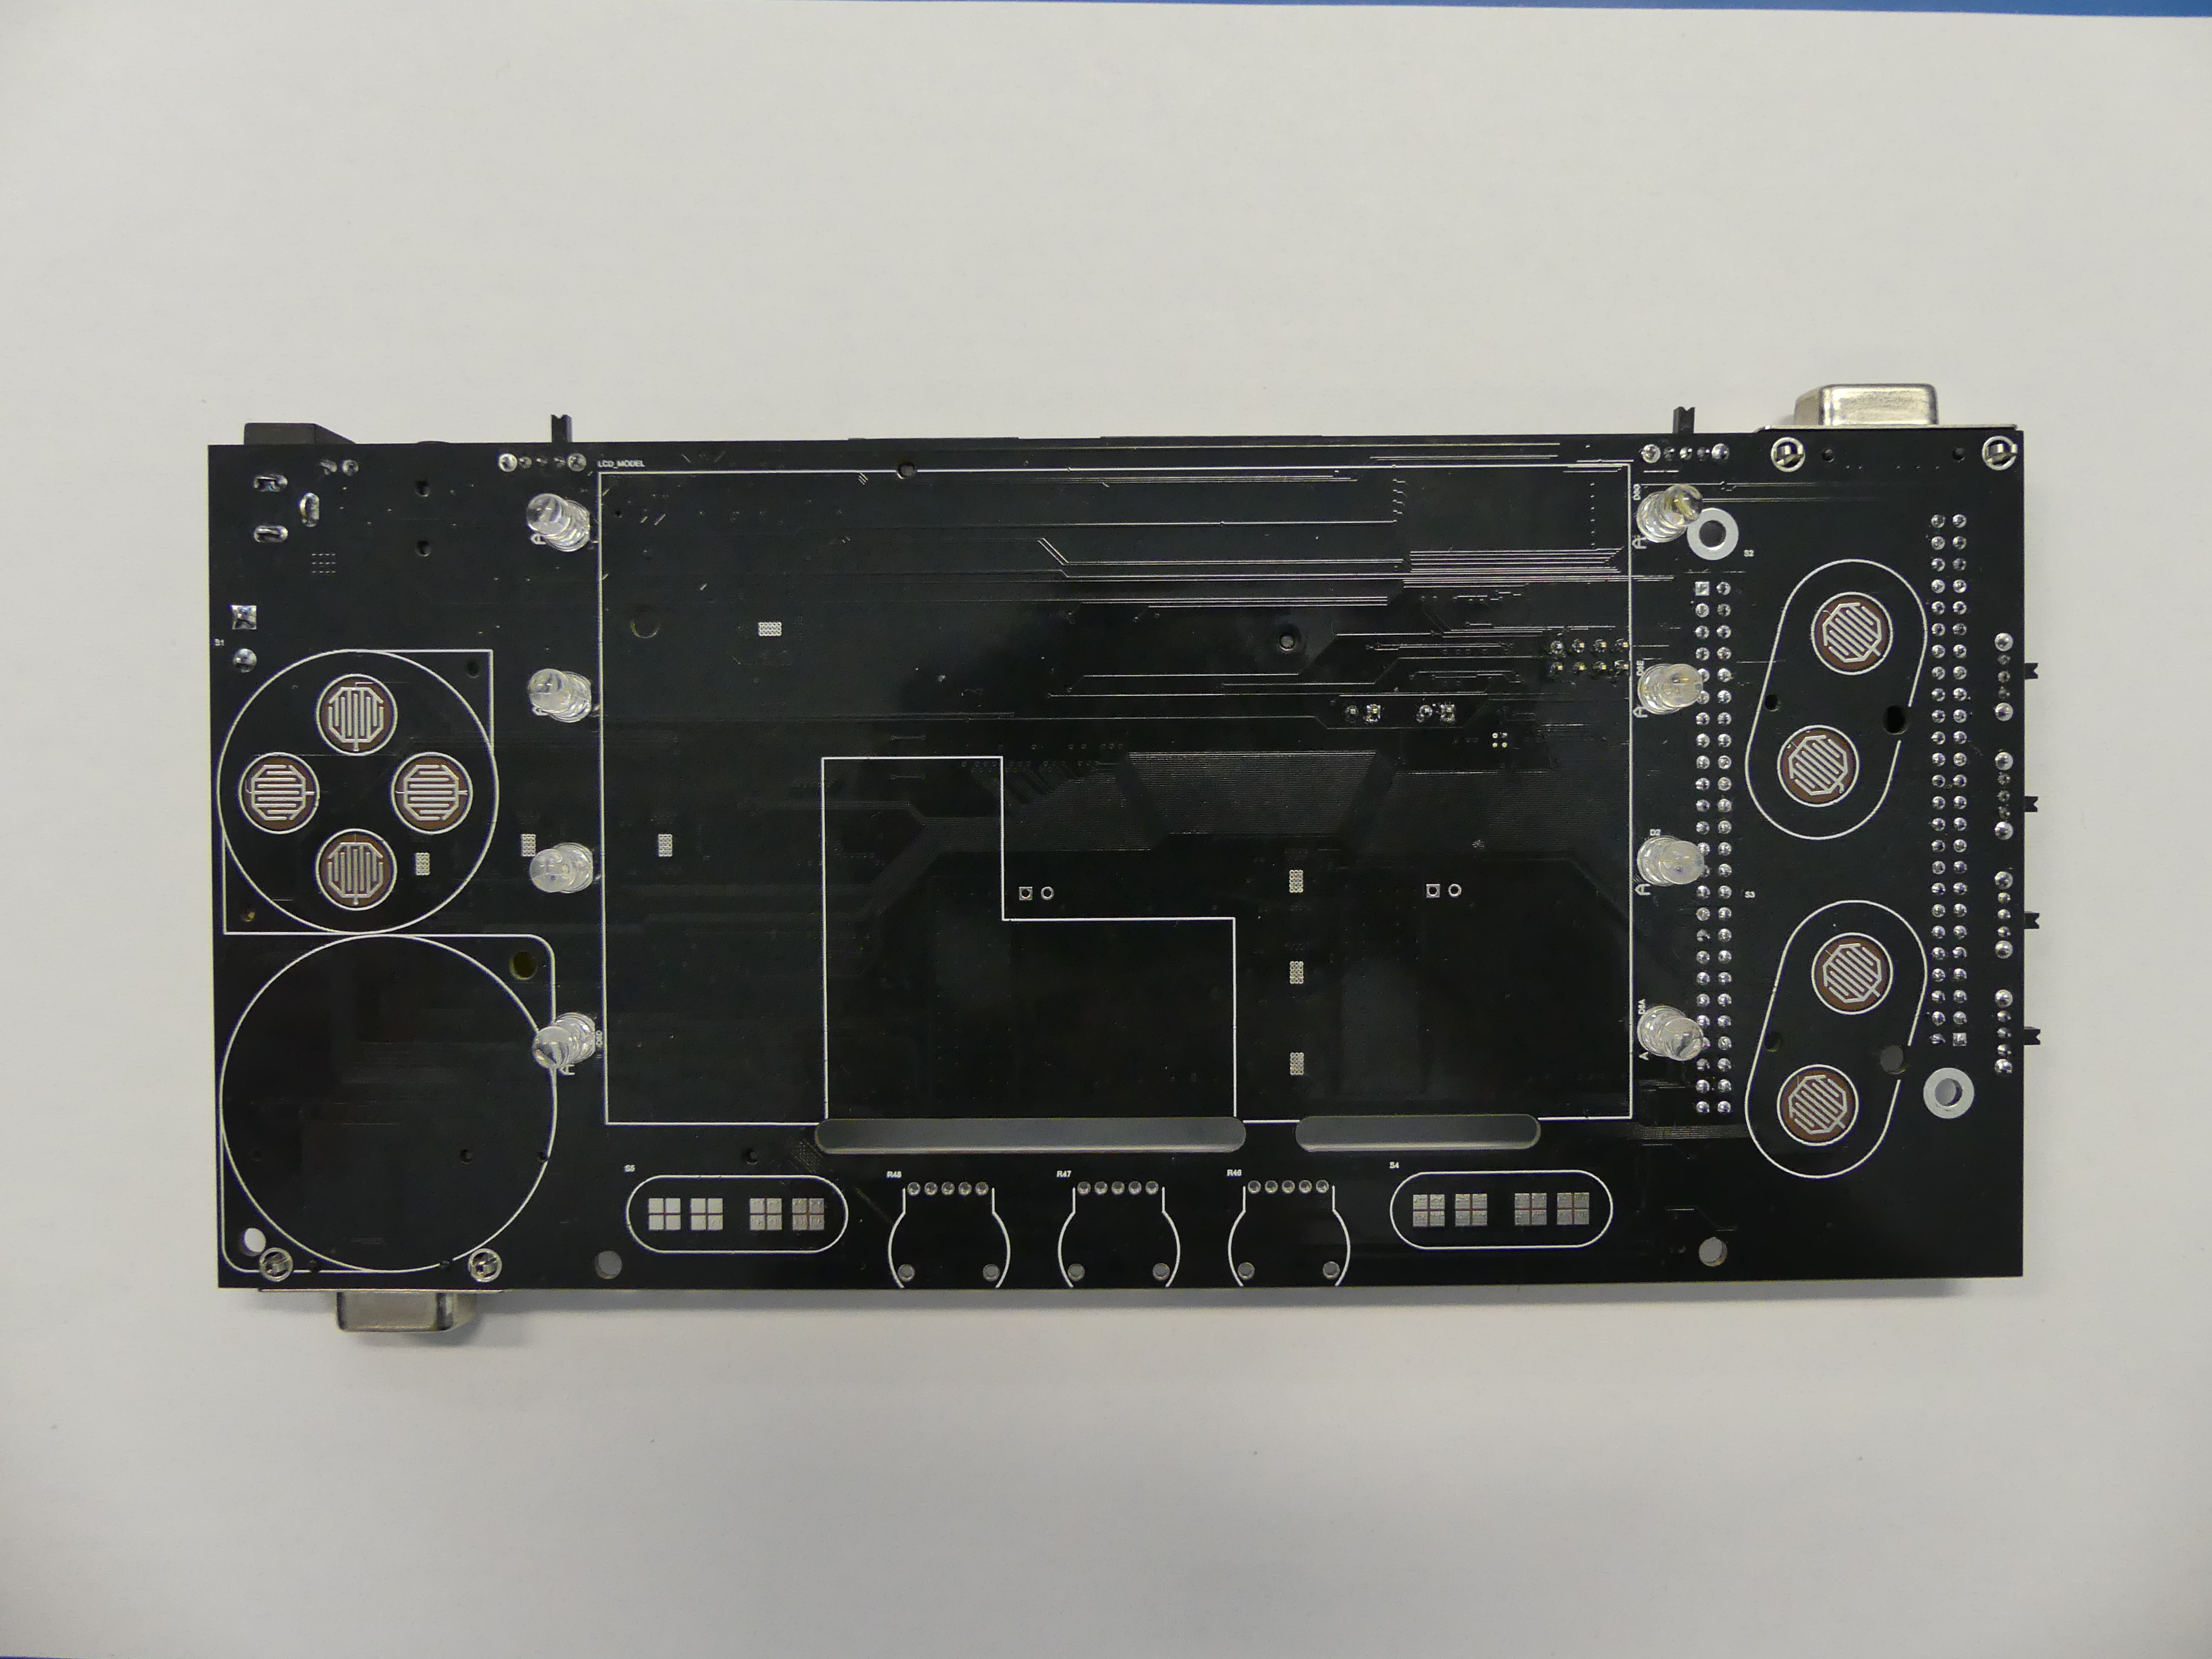
\includegraphics[width=.3\linewidth]{pics/MEGAphone_PCB_r1_populated_front} 
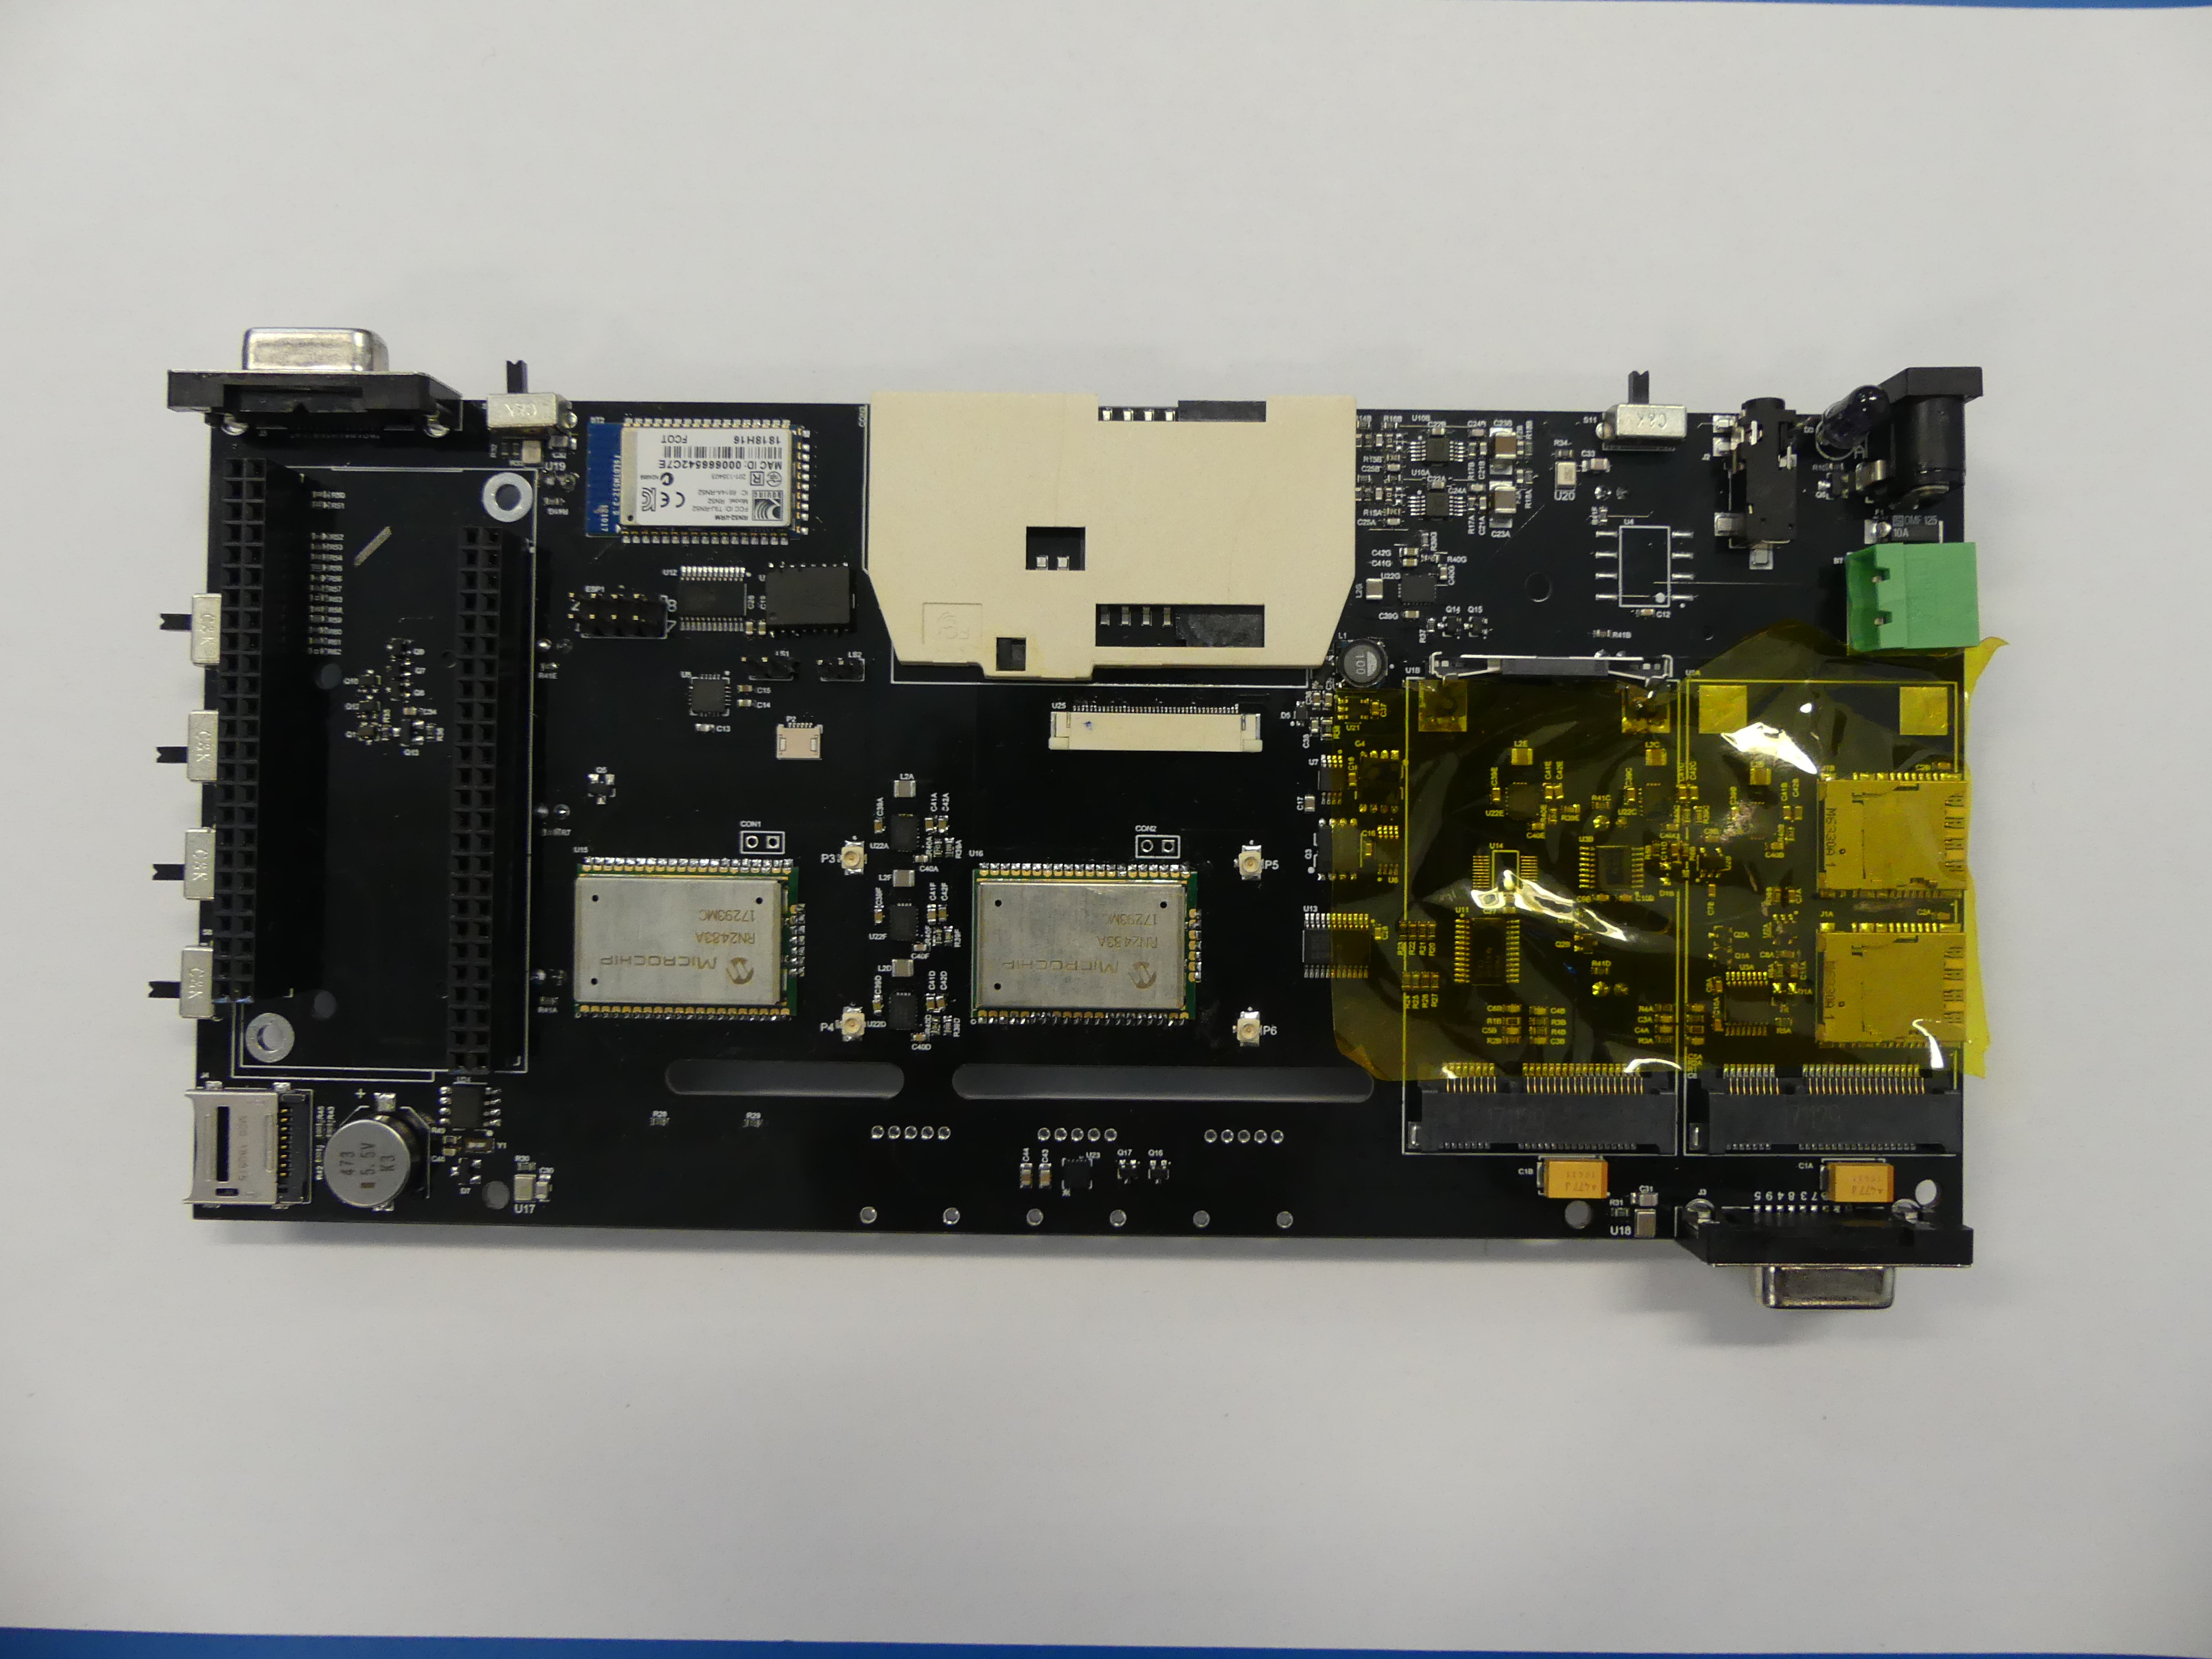
\includegraphics[width=.3\linewidth]{pics/MEGAphone_PCB_r1_populated_back} 
\end{center} 
\caption{MEGAphone PCB Revision 1 from the front and back populated with components. Front side is shown of the left.\\}
\label{MEGAphone_PCB_r1_populated}
\end{figure}


\textbf{Faults in Hardware}
\begin{enumerate}
\item The joystick connector, J3, is the wrong gender, currently it is female where as it should be male, figure \ref{MEGAphone_PCB_r1_J3}.
\item U1A and U1B, the footprint of the latch that holds the cellular modem is in the wrong position, figure \ref{MEGAphone_PCB_r1_U1A}.
\item U14 is not populated, this is the external joystick controller, figure \ref{MEGAphone_PCB_r1_U14}. 
\item U4 is currently missing, this is the Analogue-to-Digital converter for the microphone, figure \ref{MEGAphone_PCB_r1_U4}.
\item U25 needs to be moved a few millimetres to the right (when looking at the PCB face the component is mounted to) and also a couple of millimetres towards the slot which the ribbon runs through. This is to allow the ribbon cable to connect easier, figure \ref{MEGAphone_PCB_r1_U25}.
\item P2 need to be re-positioned a couple of millimetres towards the ribbon cable slot to allow the ribbon to connect easier \ref{MEGAphone_PCB_r1_P2}.
\item U15 may need to be moved a few millimetres to the left (when looking at the component) to allow for the ribbon cable to reach P2 without rubbing on U15 figure \ref{MEGAphone_PCB_r1_P2}.
\item LED power indicator are slightly too close together to allow the screen cover to fit between them \ref{MEGAphone_PCB_r1_LED}.
\item U9 which is the SPI flash chip, the footprint is wrong i.e. doesn't match the part, figure \ref{MEGAphone_PCB_r1_U9}.
\item R46, R47 and R48, the thumb wheels for volume control, are missing and currently on back order, figure \ref{MEGAphone_PCB_r1_R49_R48_R47}.
\item Found the PCB is outputting over 6.45 Volts where it should be outputting 3.3V. \\
\end{enumerate}

\begin{figure} \begin{center}
\includegraphics[width=.3\linewidth]{pics/MEGAphone_PCB_r1_J3} 
\end{center} 
\caption{Close up of Joystick connector J3, which should be a male connector.\\}
\label{MEGAphone_PCB_r1_J3}
\end{figure}

\begin{figure} \begin{center}
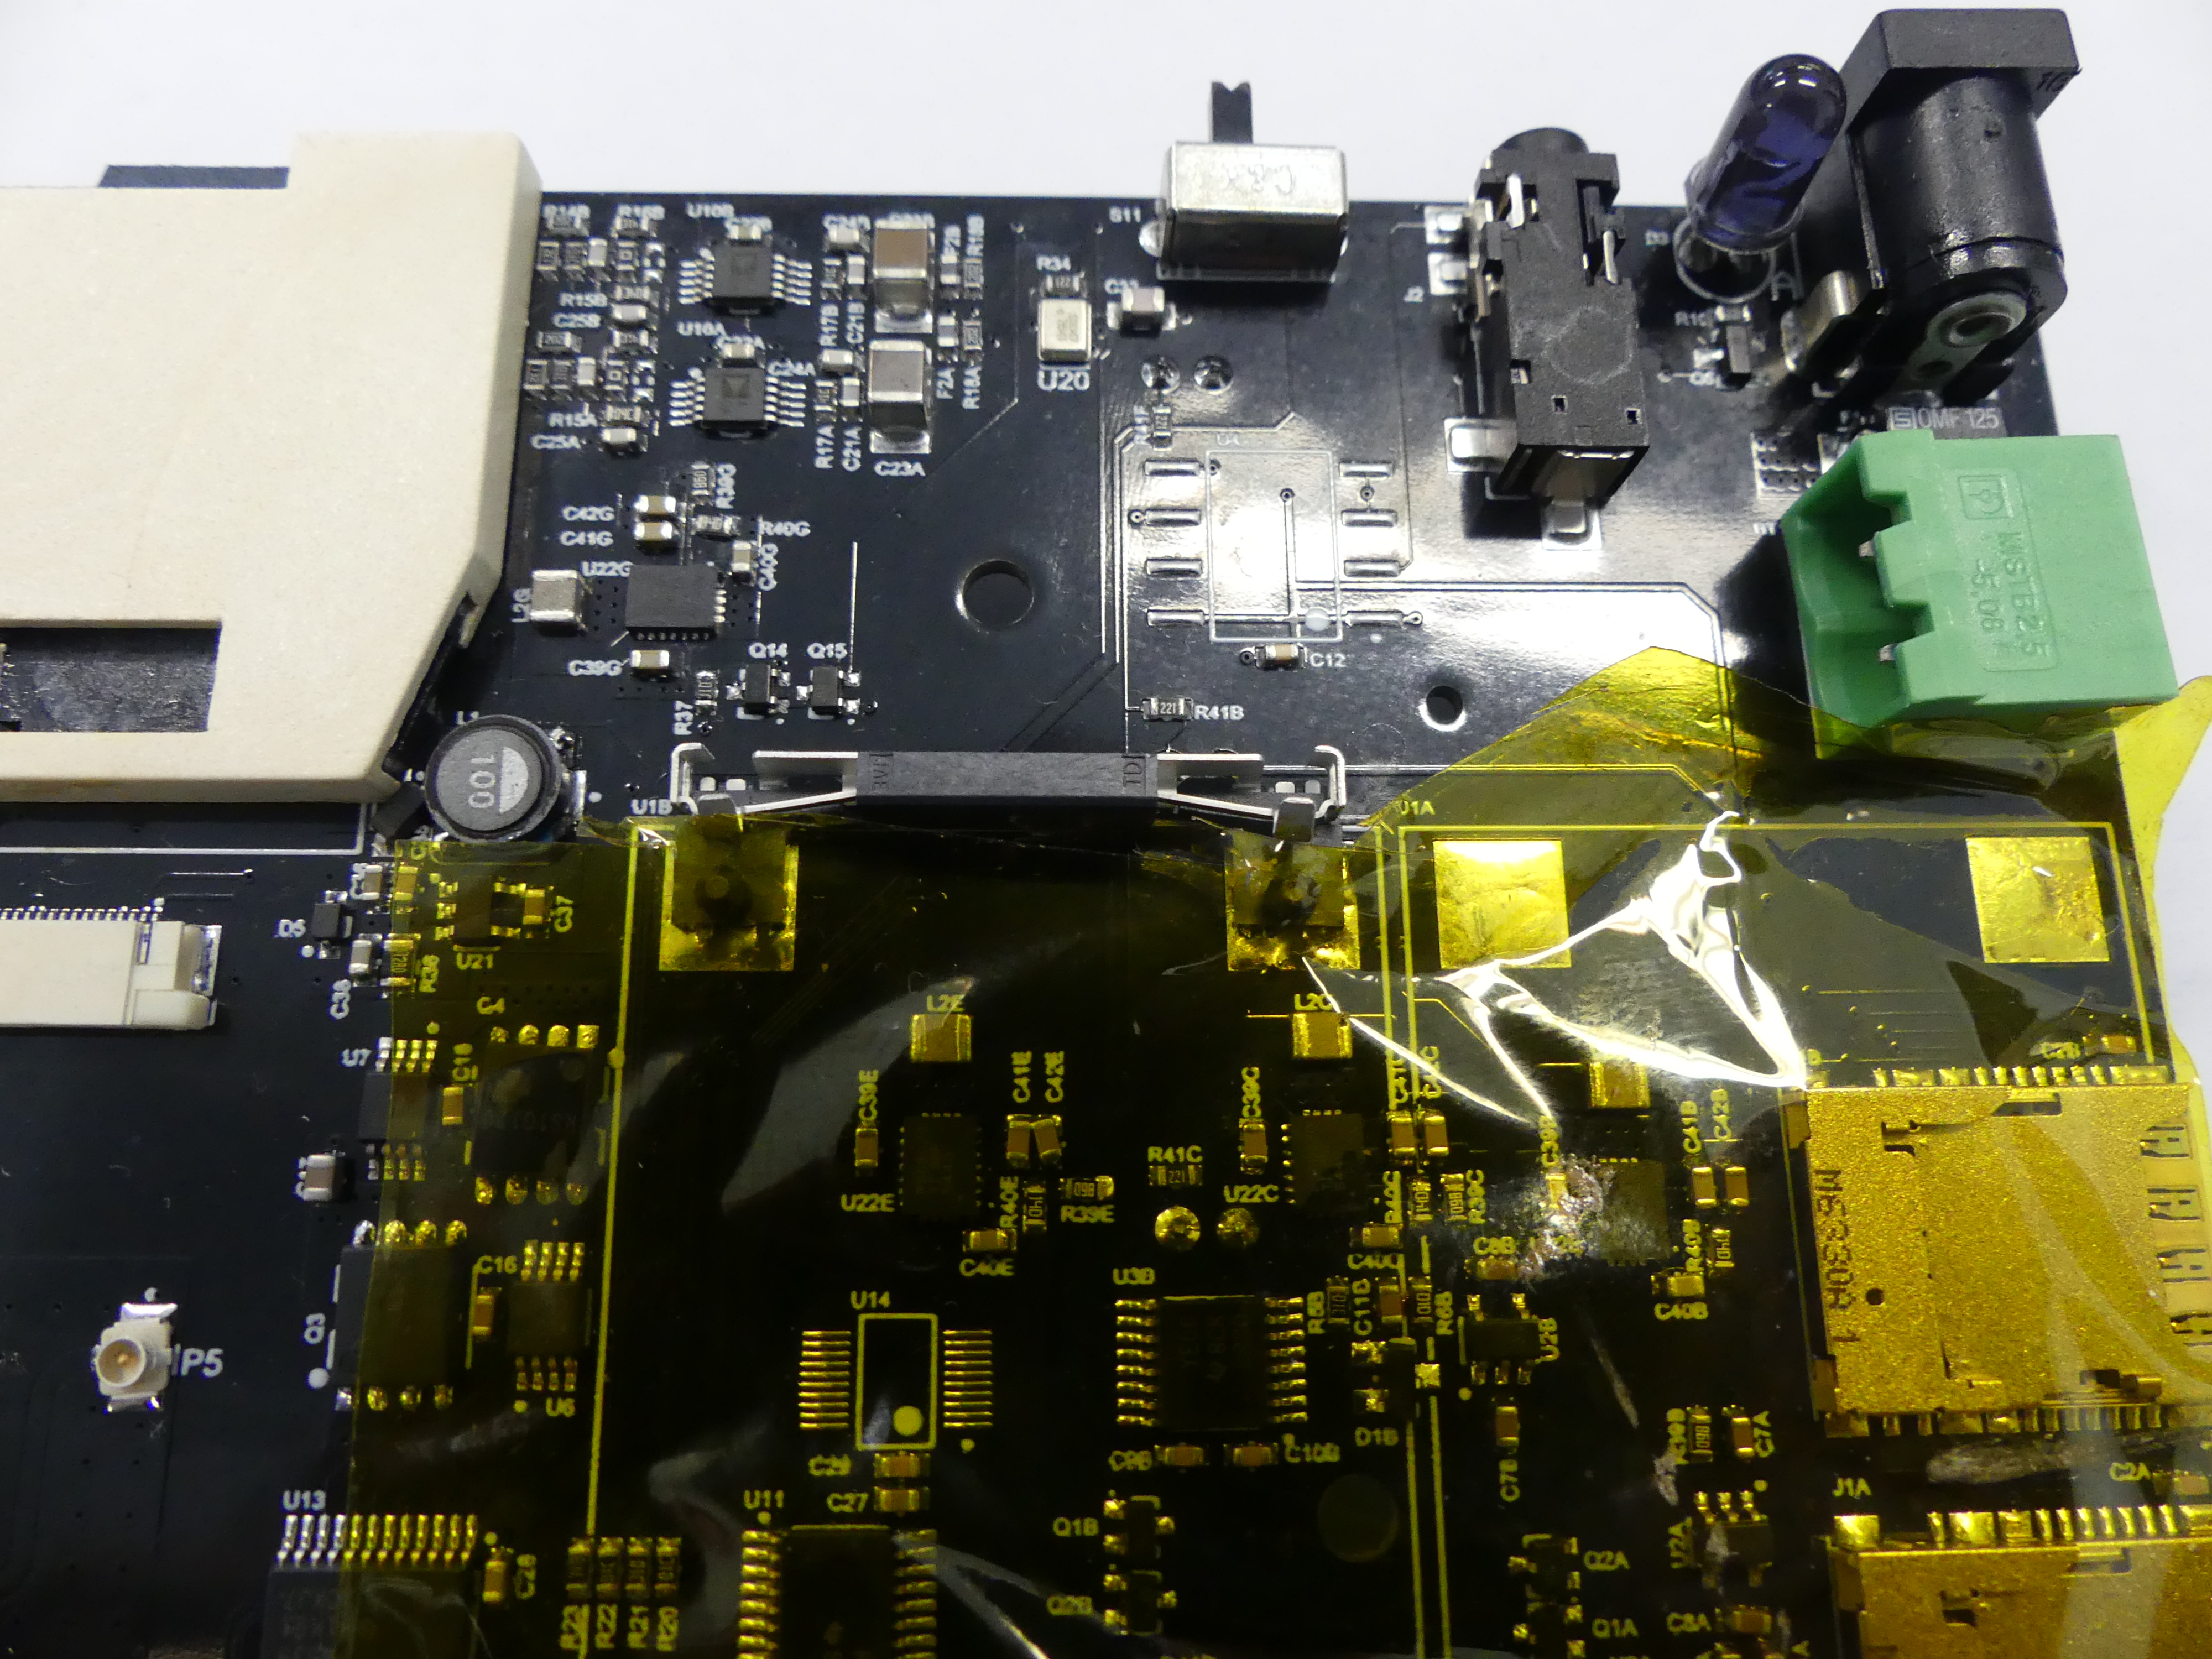
\includegraphics[width=.3\linewidth]{pics/MEGAphone_PCB_r1_U1A} 
\end{center} 
\caption{Close up showing the latch installed in U1B but not U1A.\\}
\label{MEGAphone_PCB_r1_U1A}
\end{figure}

\begin{figure} \begin{center}
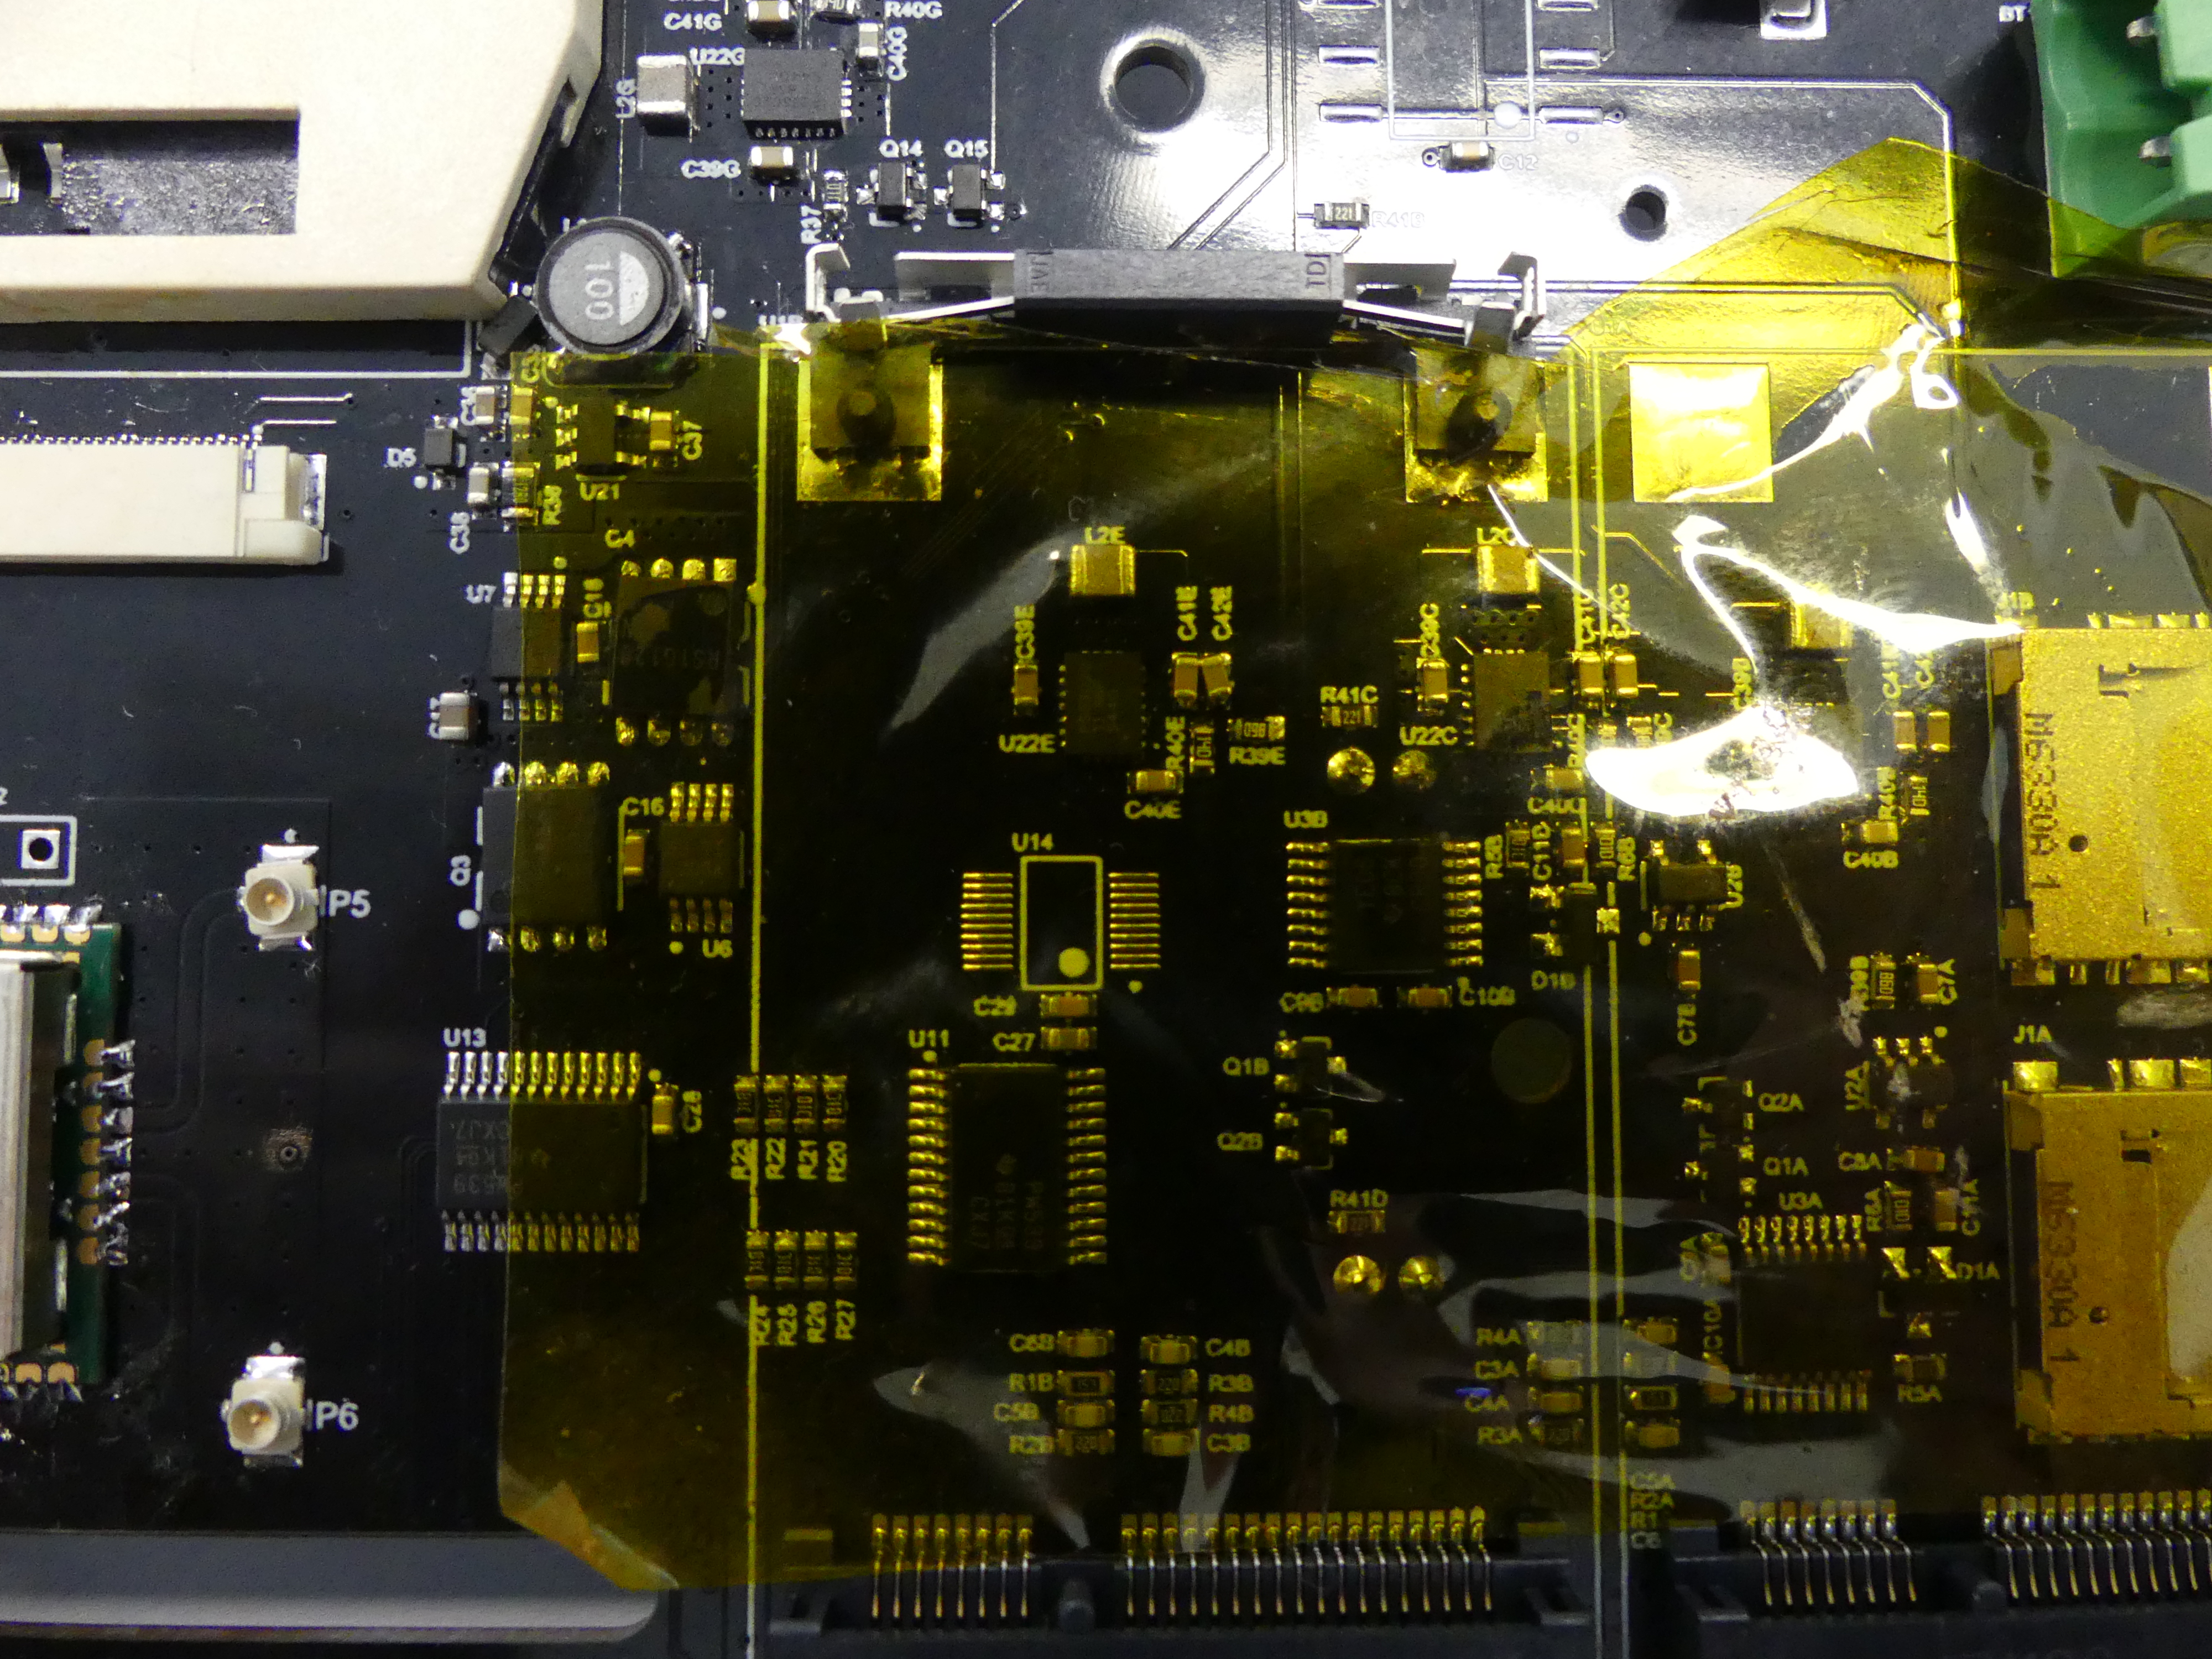
\includegraphics[width=.3\linewidth]{pics/MEGAphone_PCB_r1_U14} 
\end{center} 
\caption{Close up showing unpopulated component U14.\\}
\label{MEGAphone_PCB_r1_U14}
\end{figure}

\begin{figure} \begin{center}
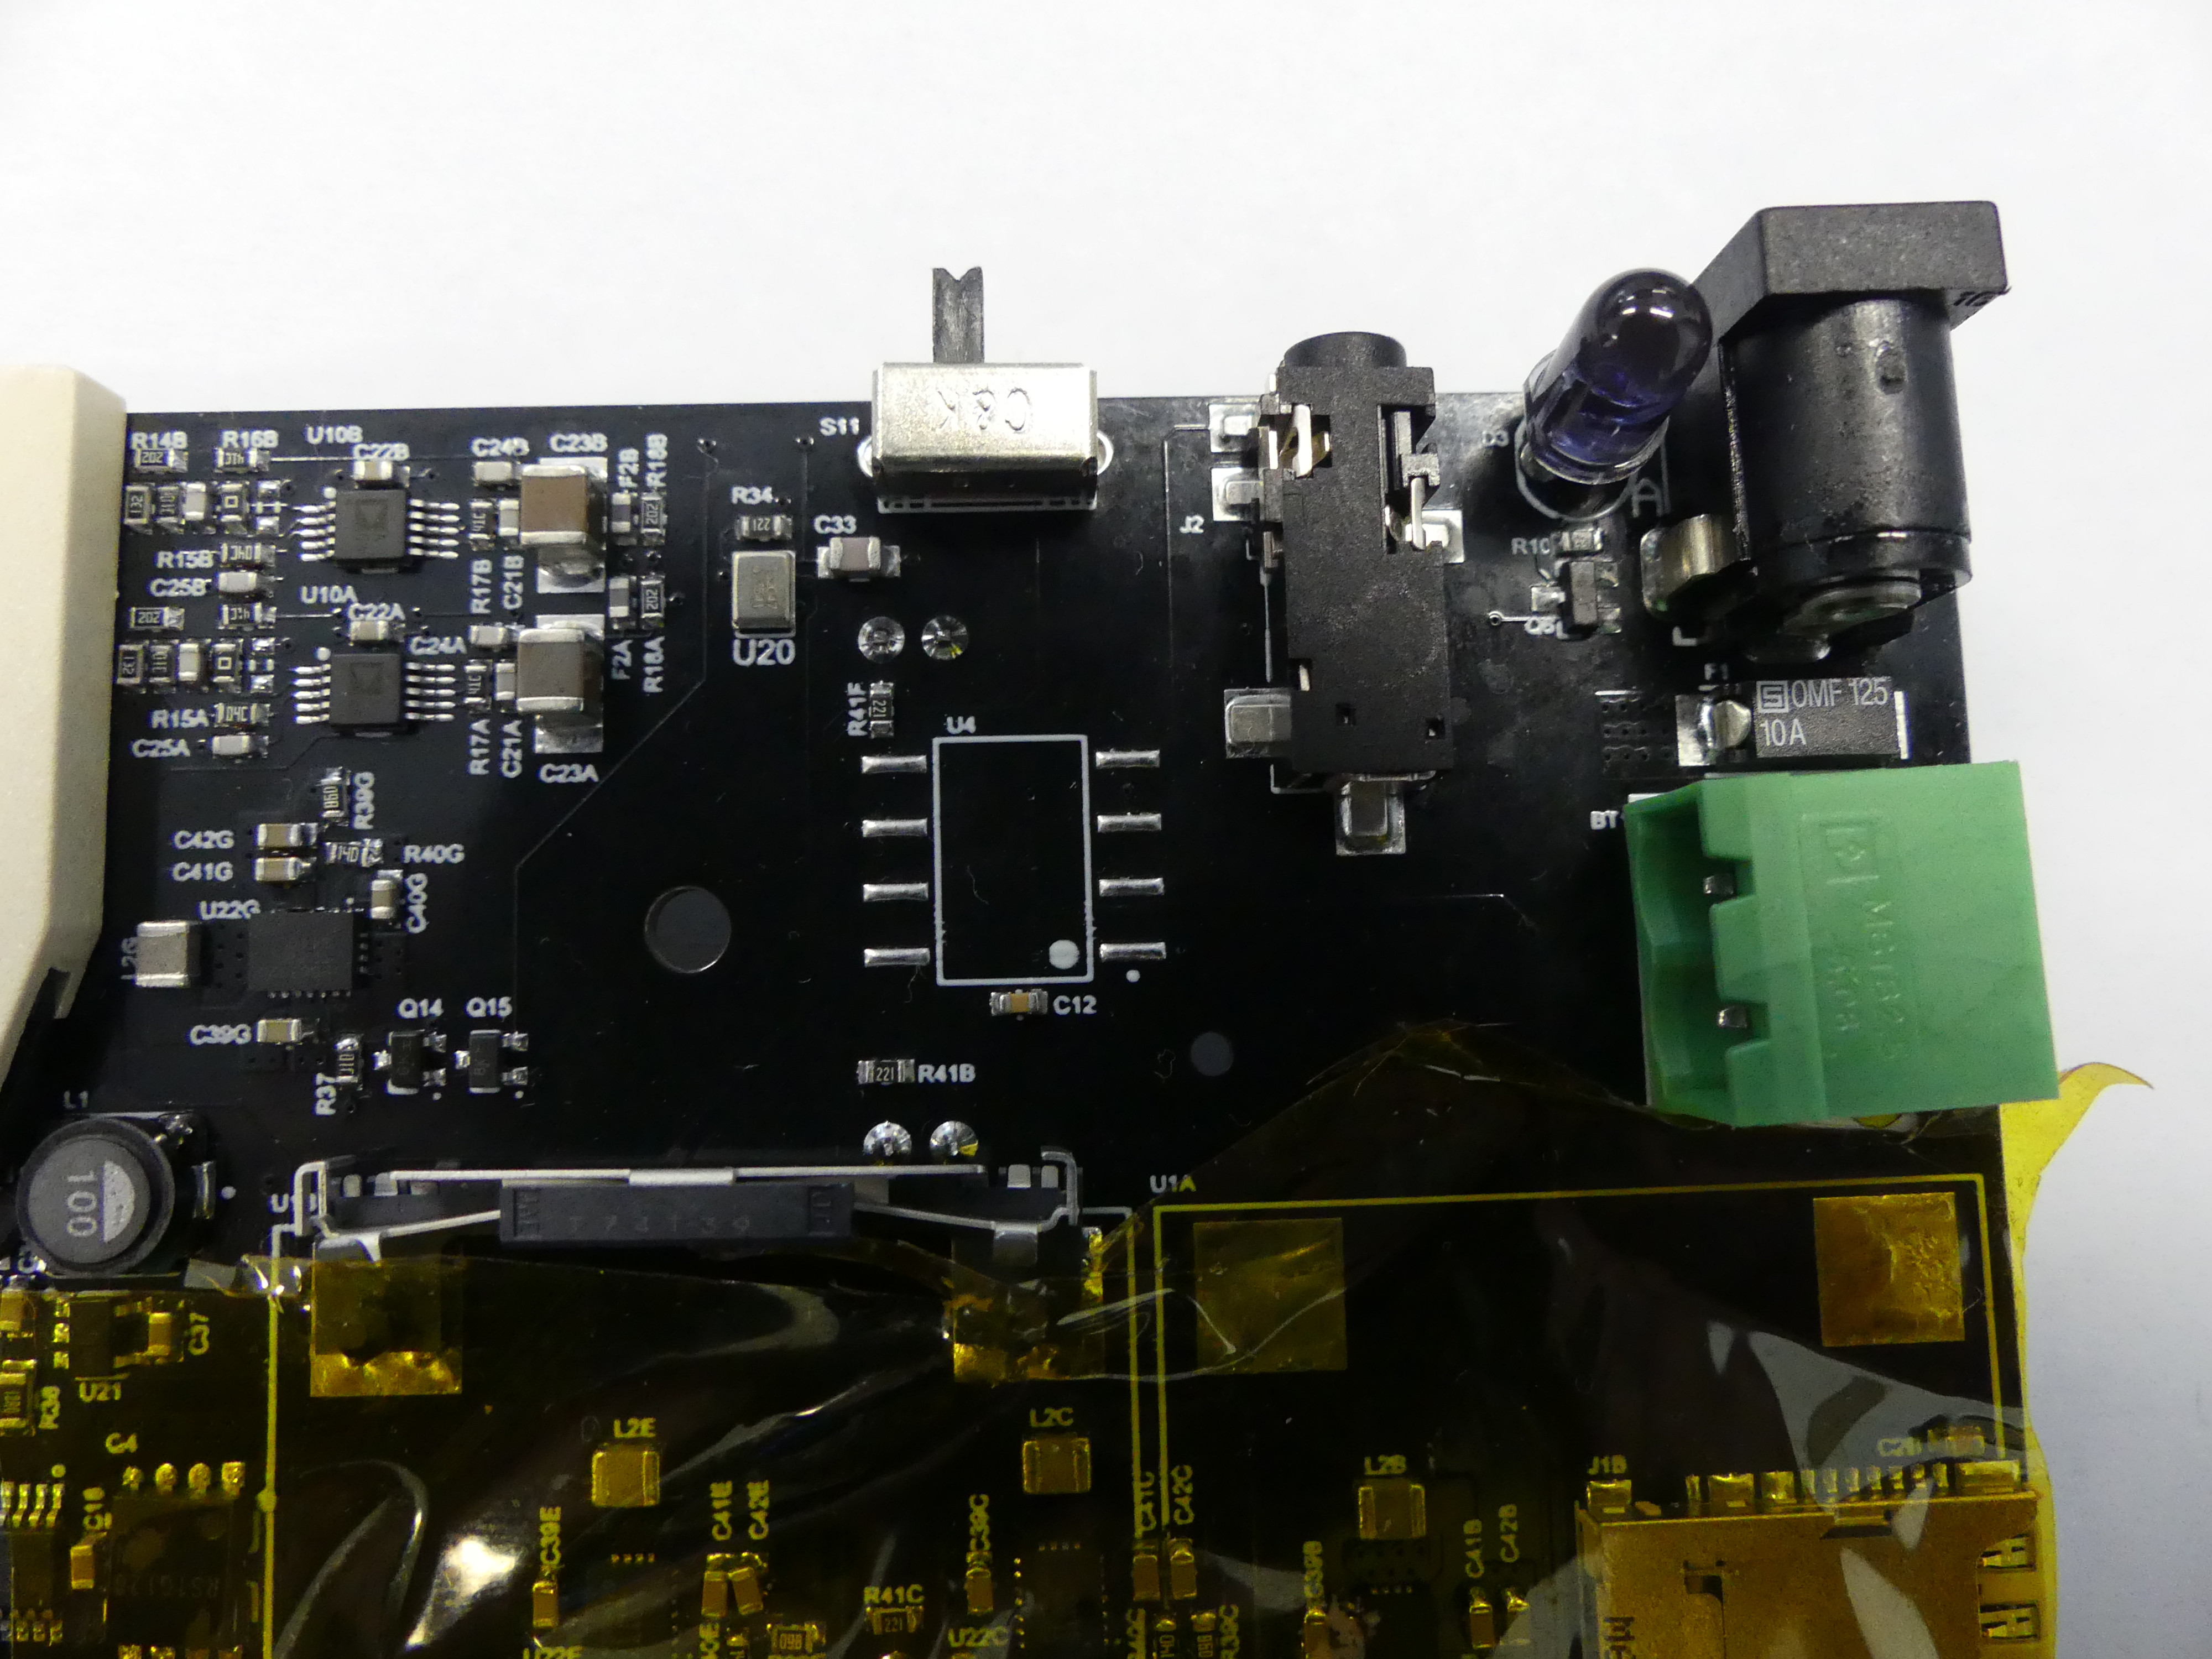
\includegraphics[width=.3\linewidth]{pics/MEGAphone_PCB_r1_U4} 
\end{center} 
\caption{Close up showing unpopulated component U4.\\}
\label{MEGAphone_PCB_r1_U4}
\end{figure}

\begin{figure} \begin{center}
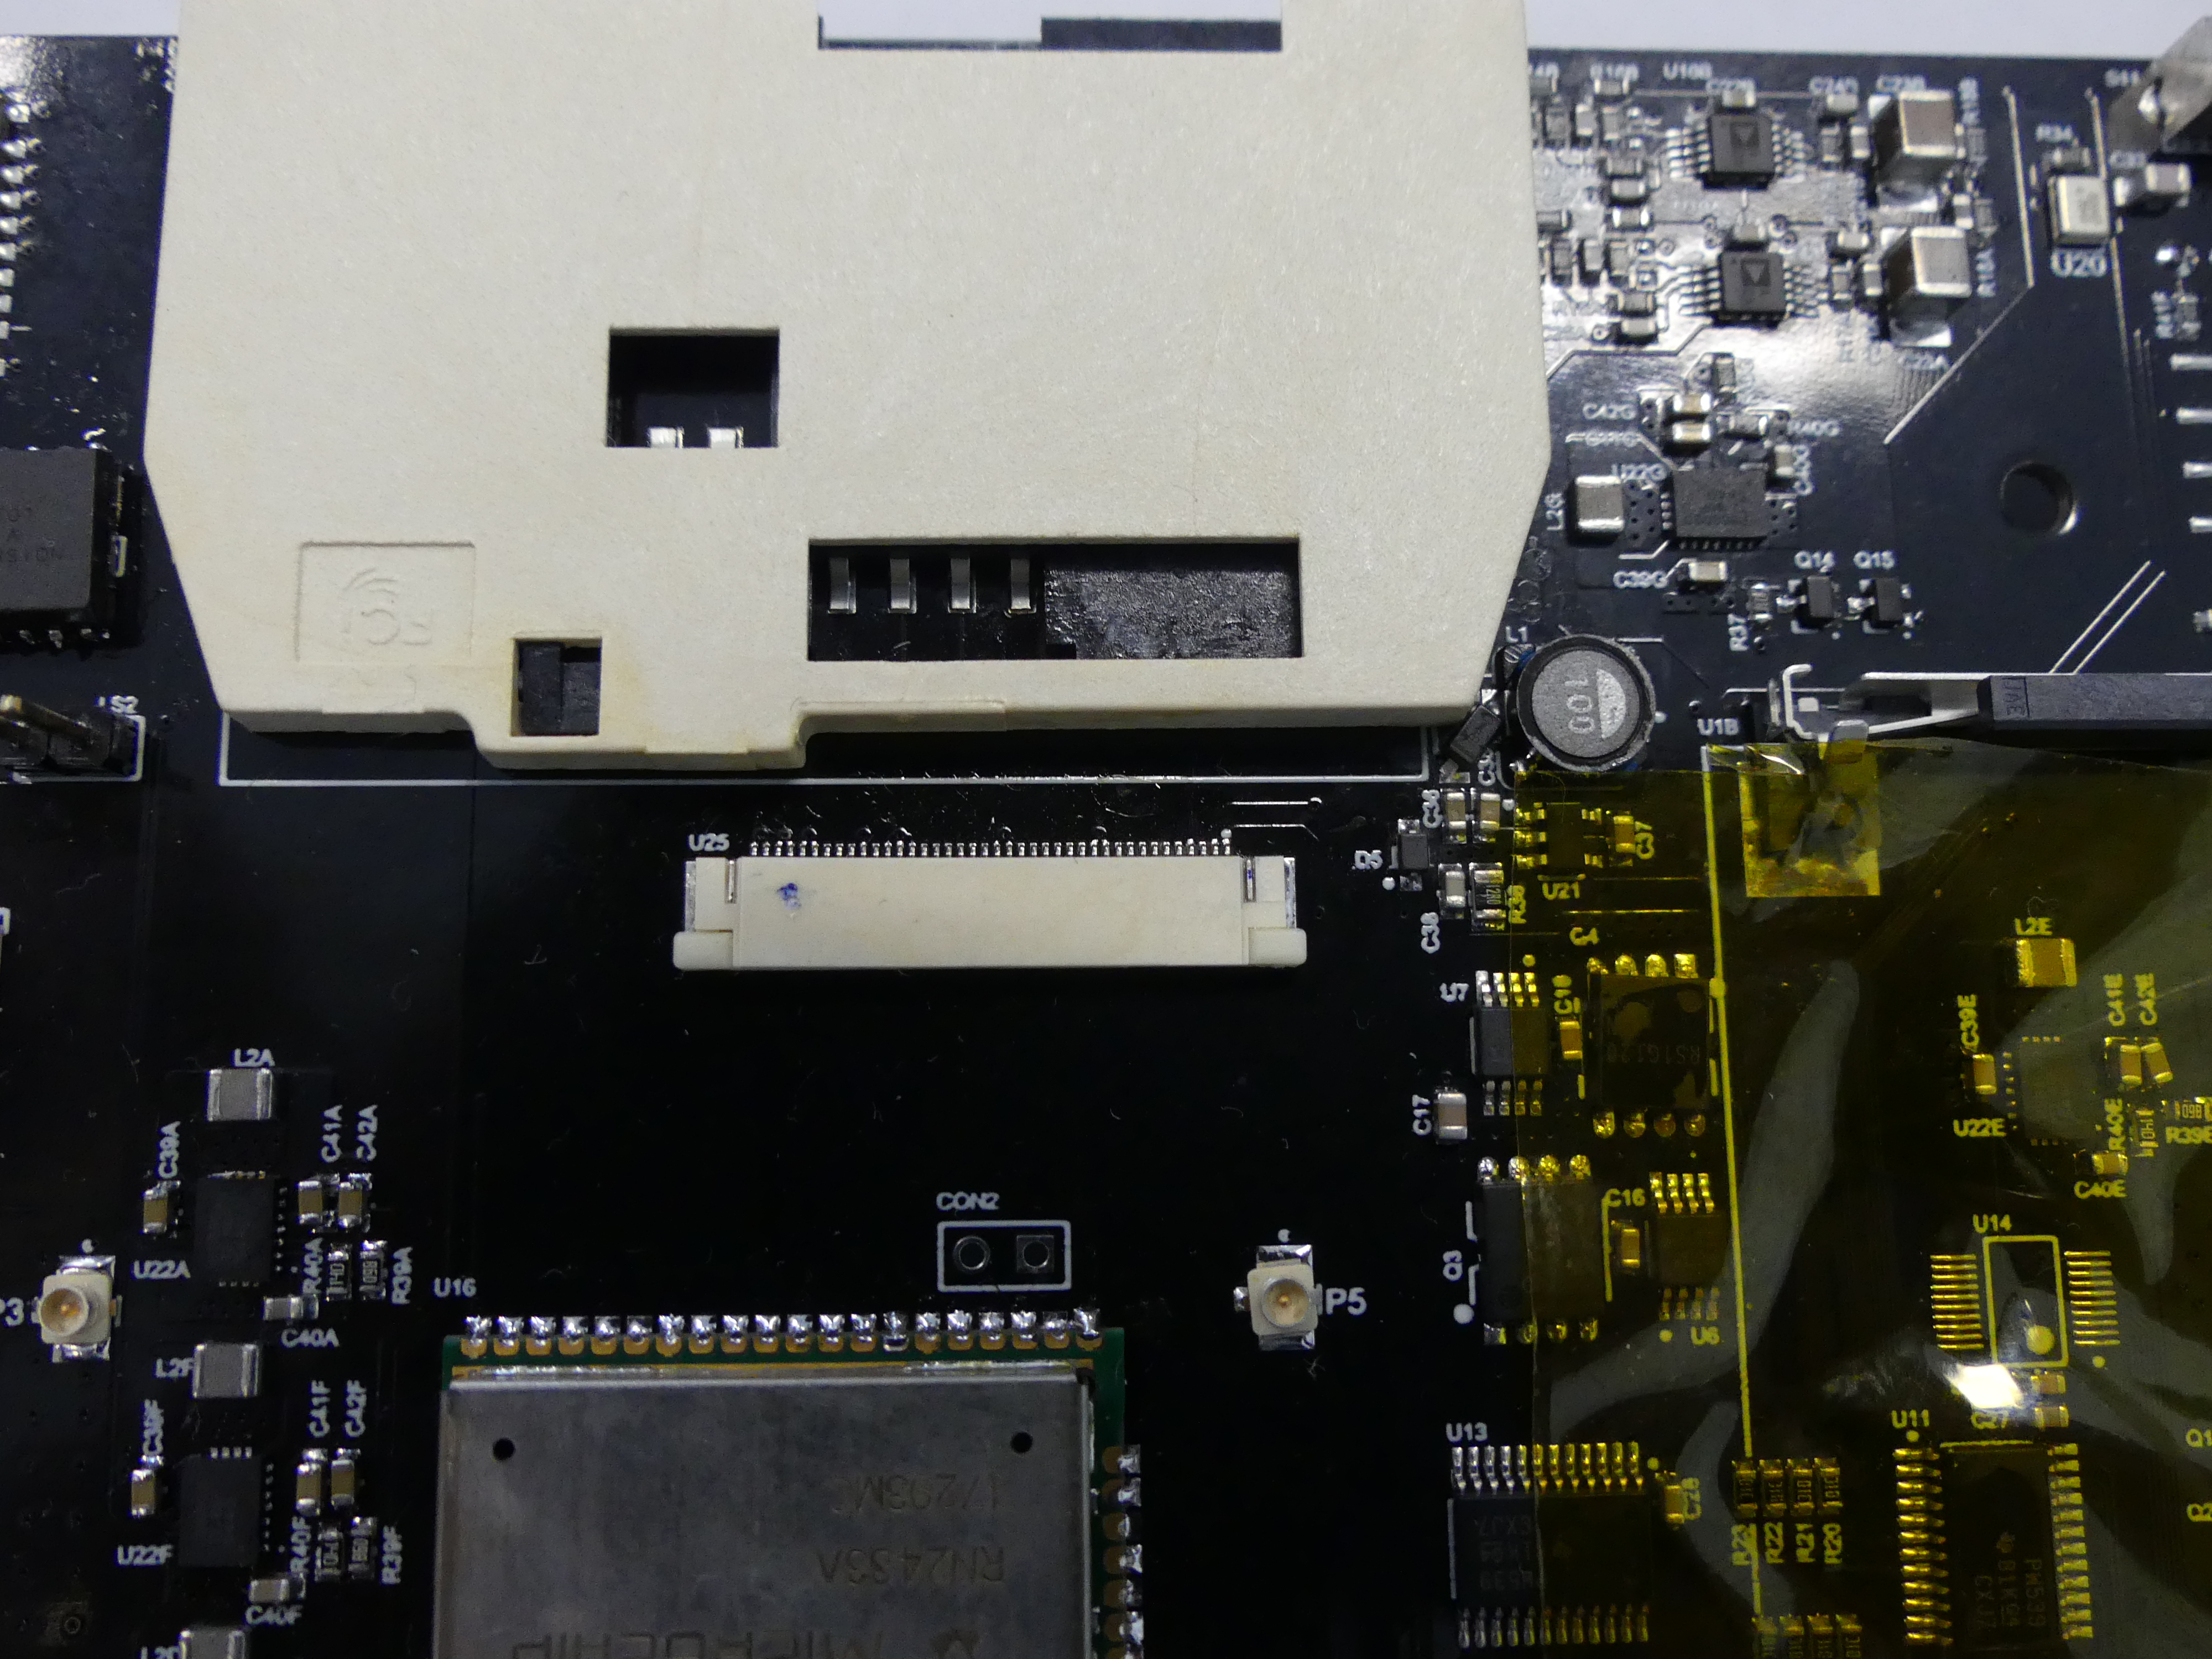
\includegraphics[width=.3\linewidth]{pics/MEGAphone_PCB_r1_U25}
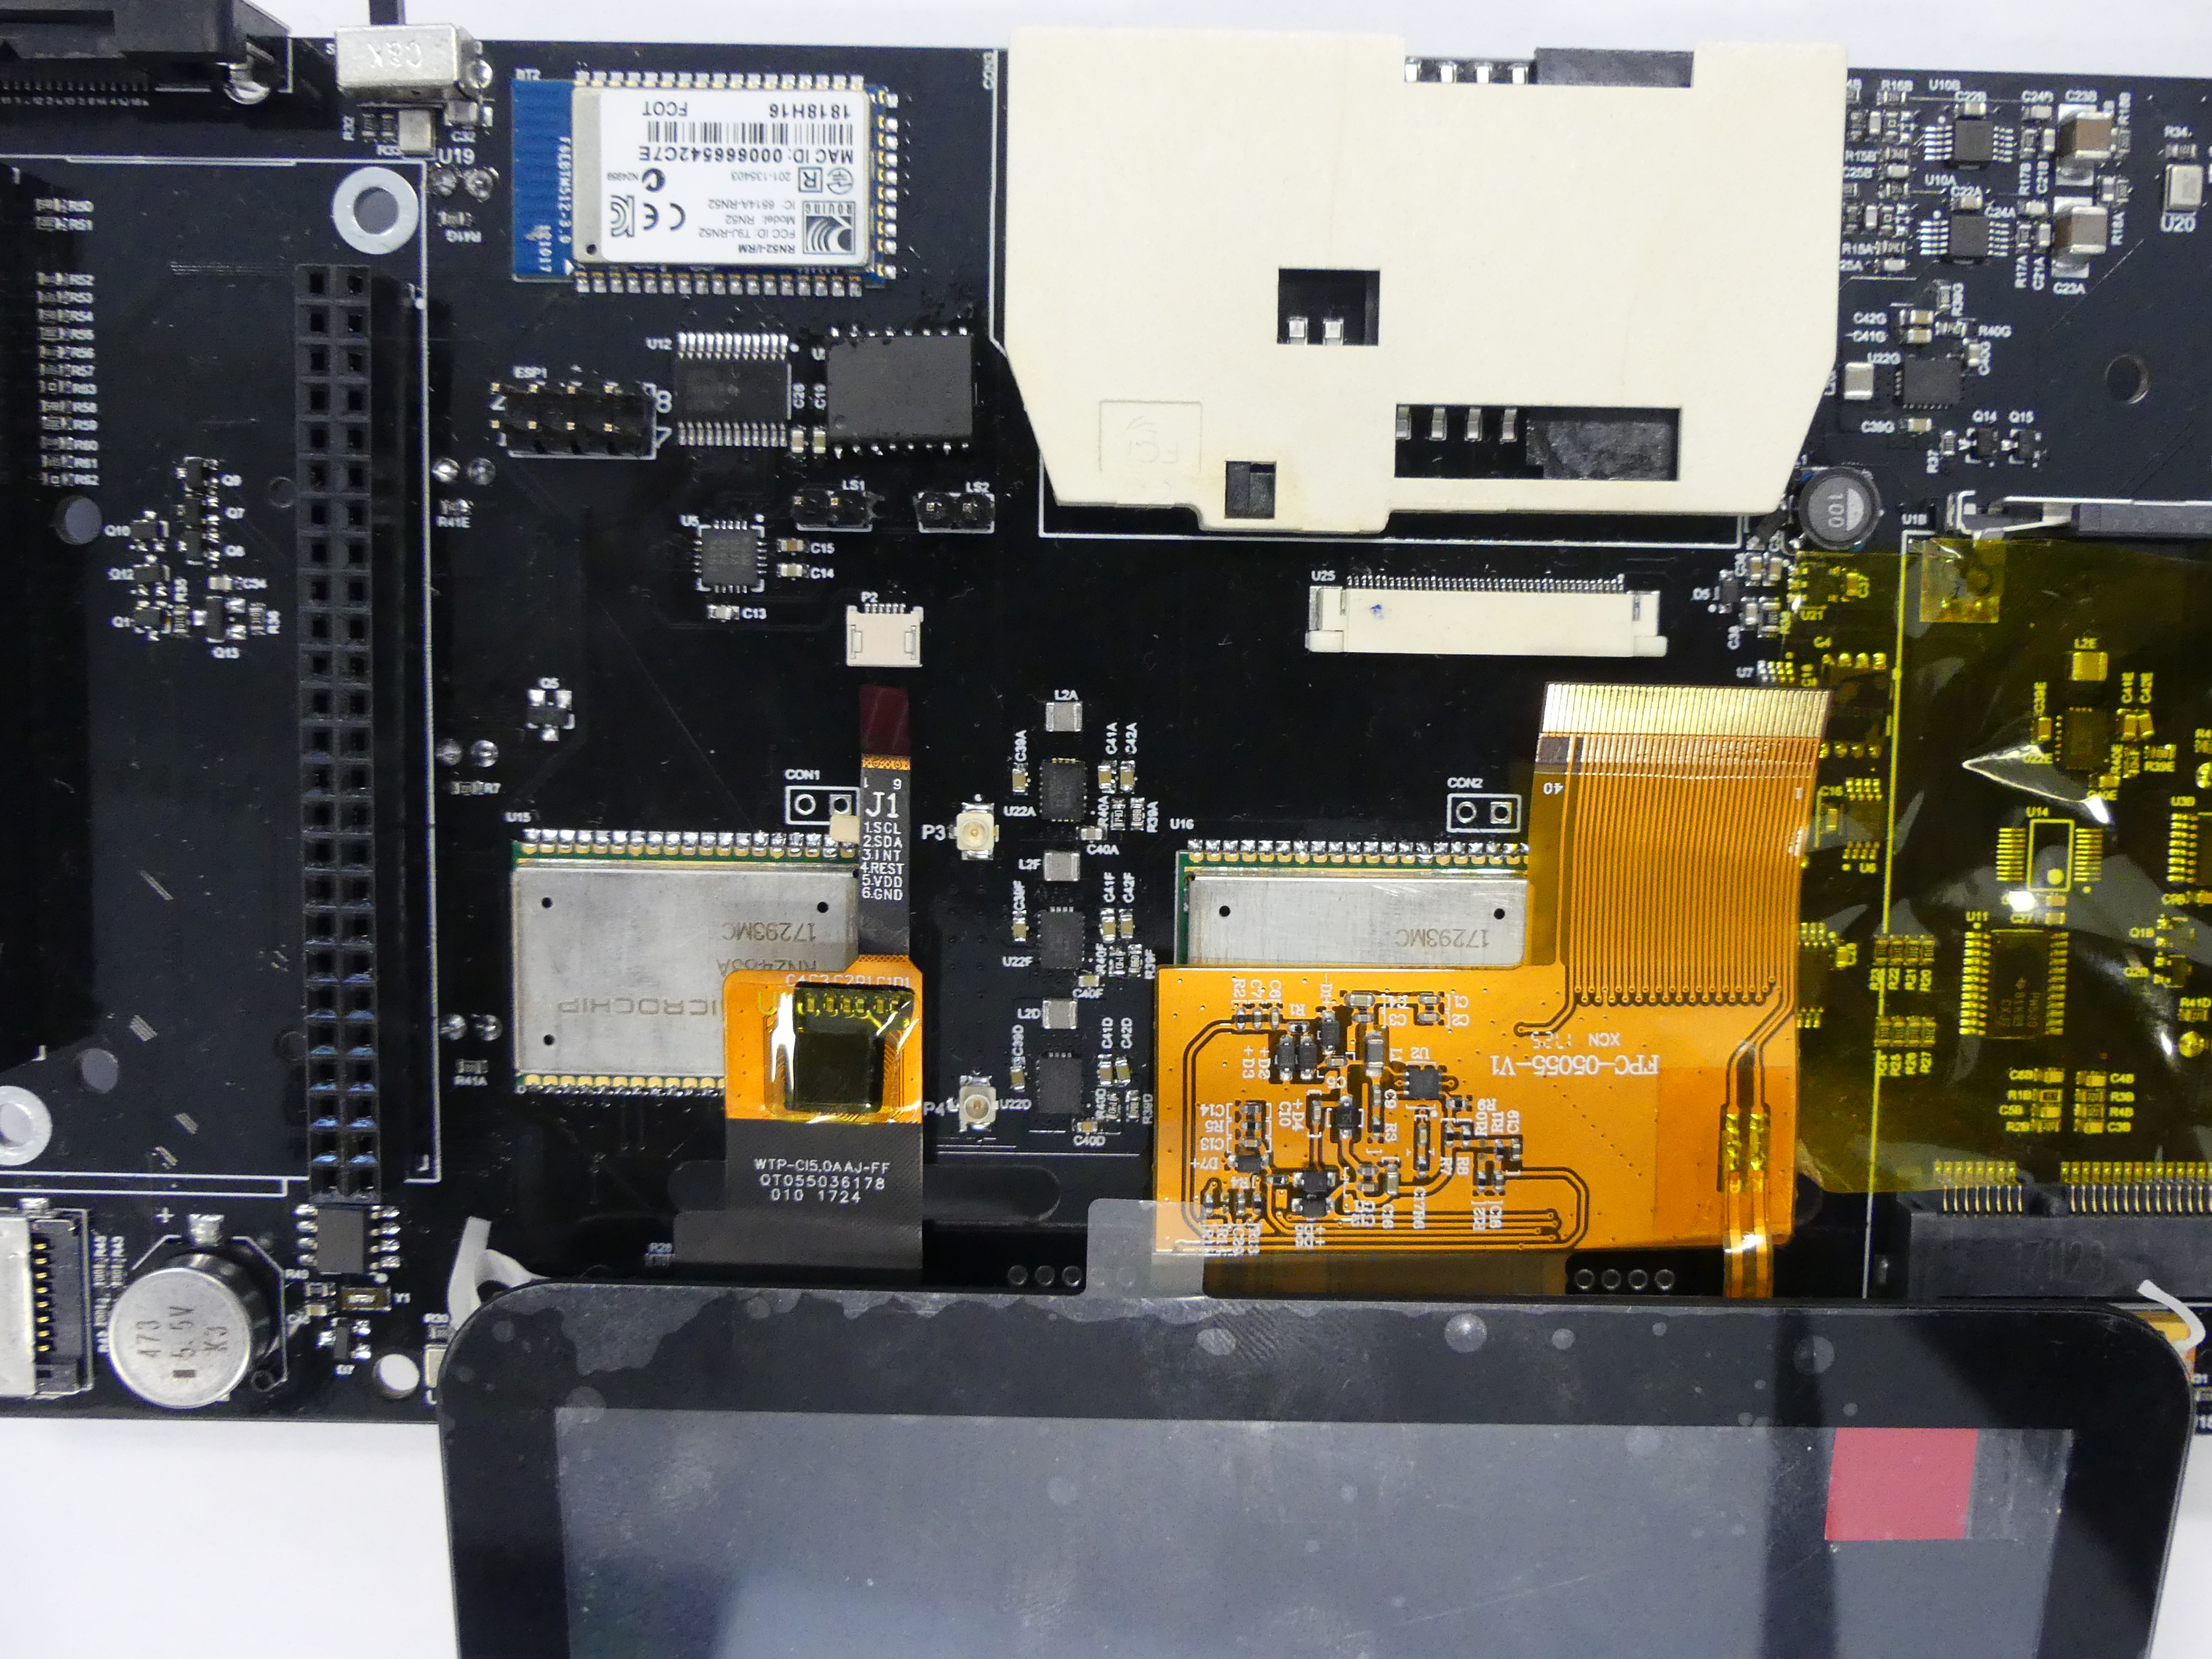
\includegraphics[width=.3\linewidth]{pics/MEGAphone_PCB_r1_U25_P2_ribbon}
\end{center} 
\caption{Close up showing component U25 as well with as the ribbon connector for the screen. U25 needs to be re-positioned.\\}
\label{MEGAphone_PCB_r1_U25}
\end{figure}

\begin{figure} \begin{center}
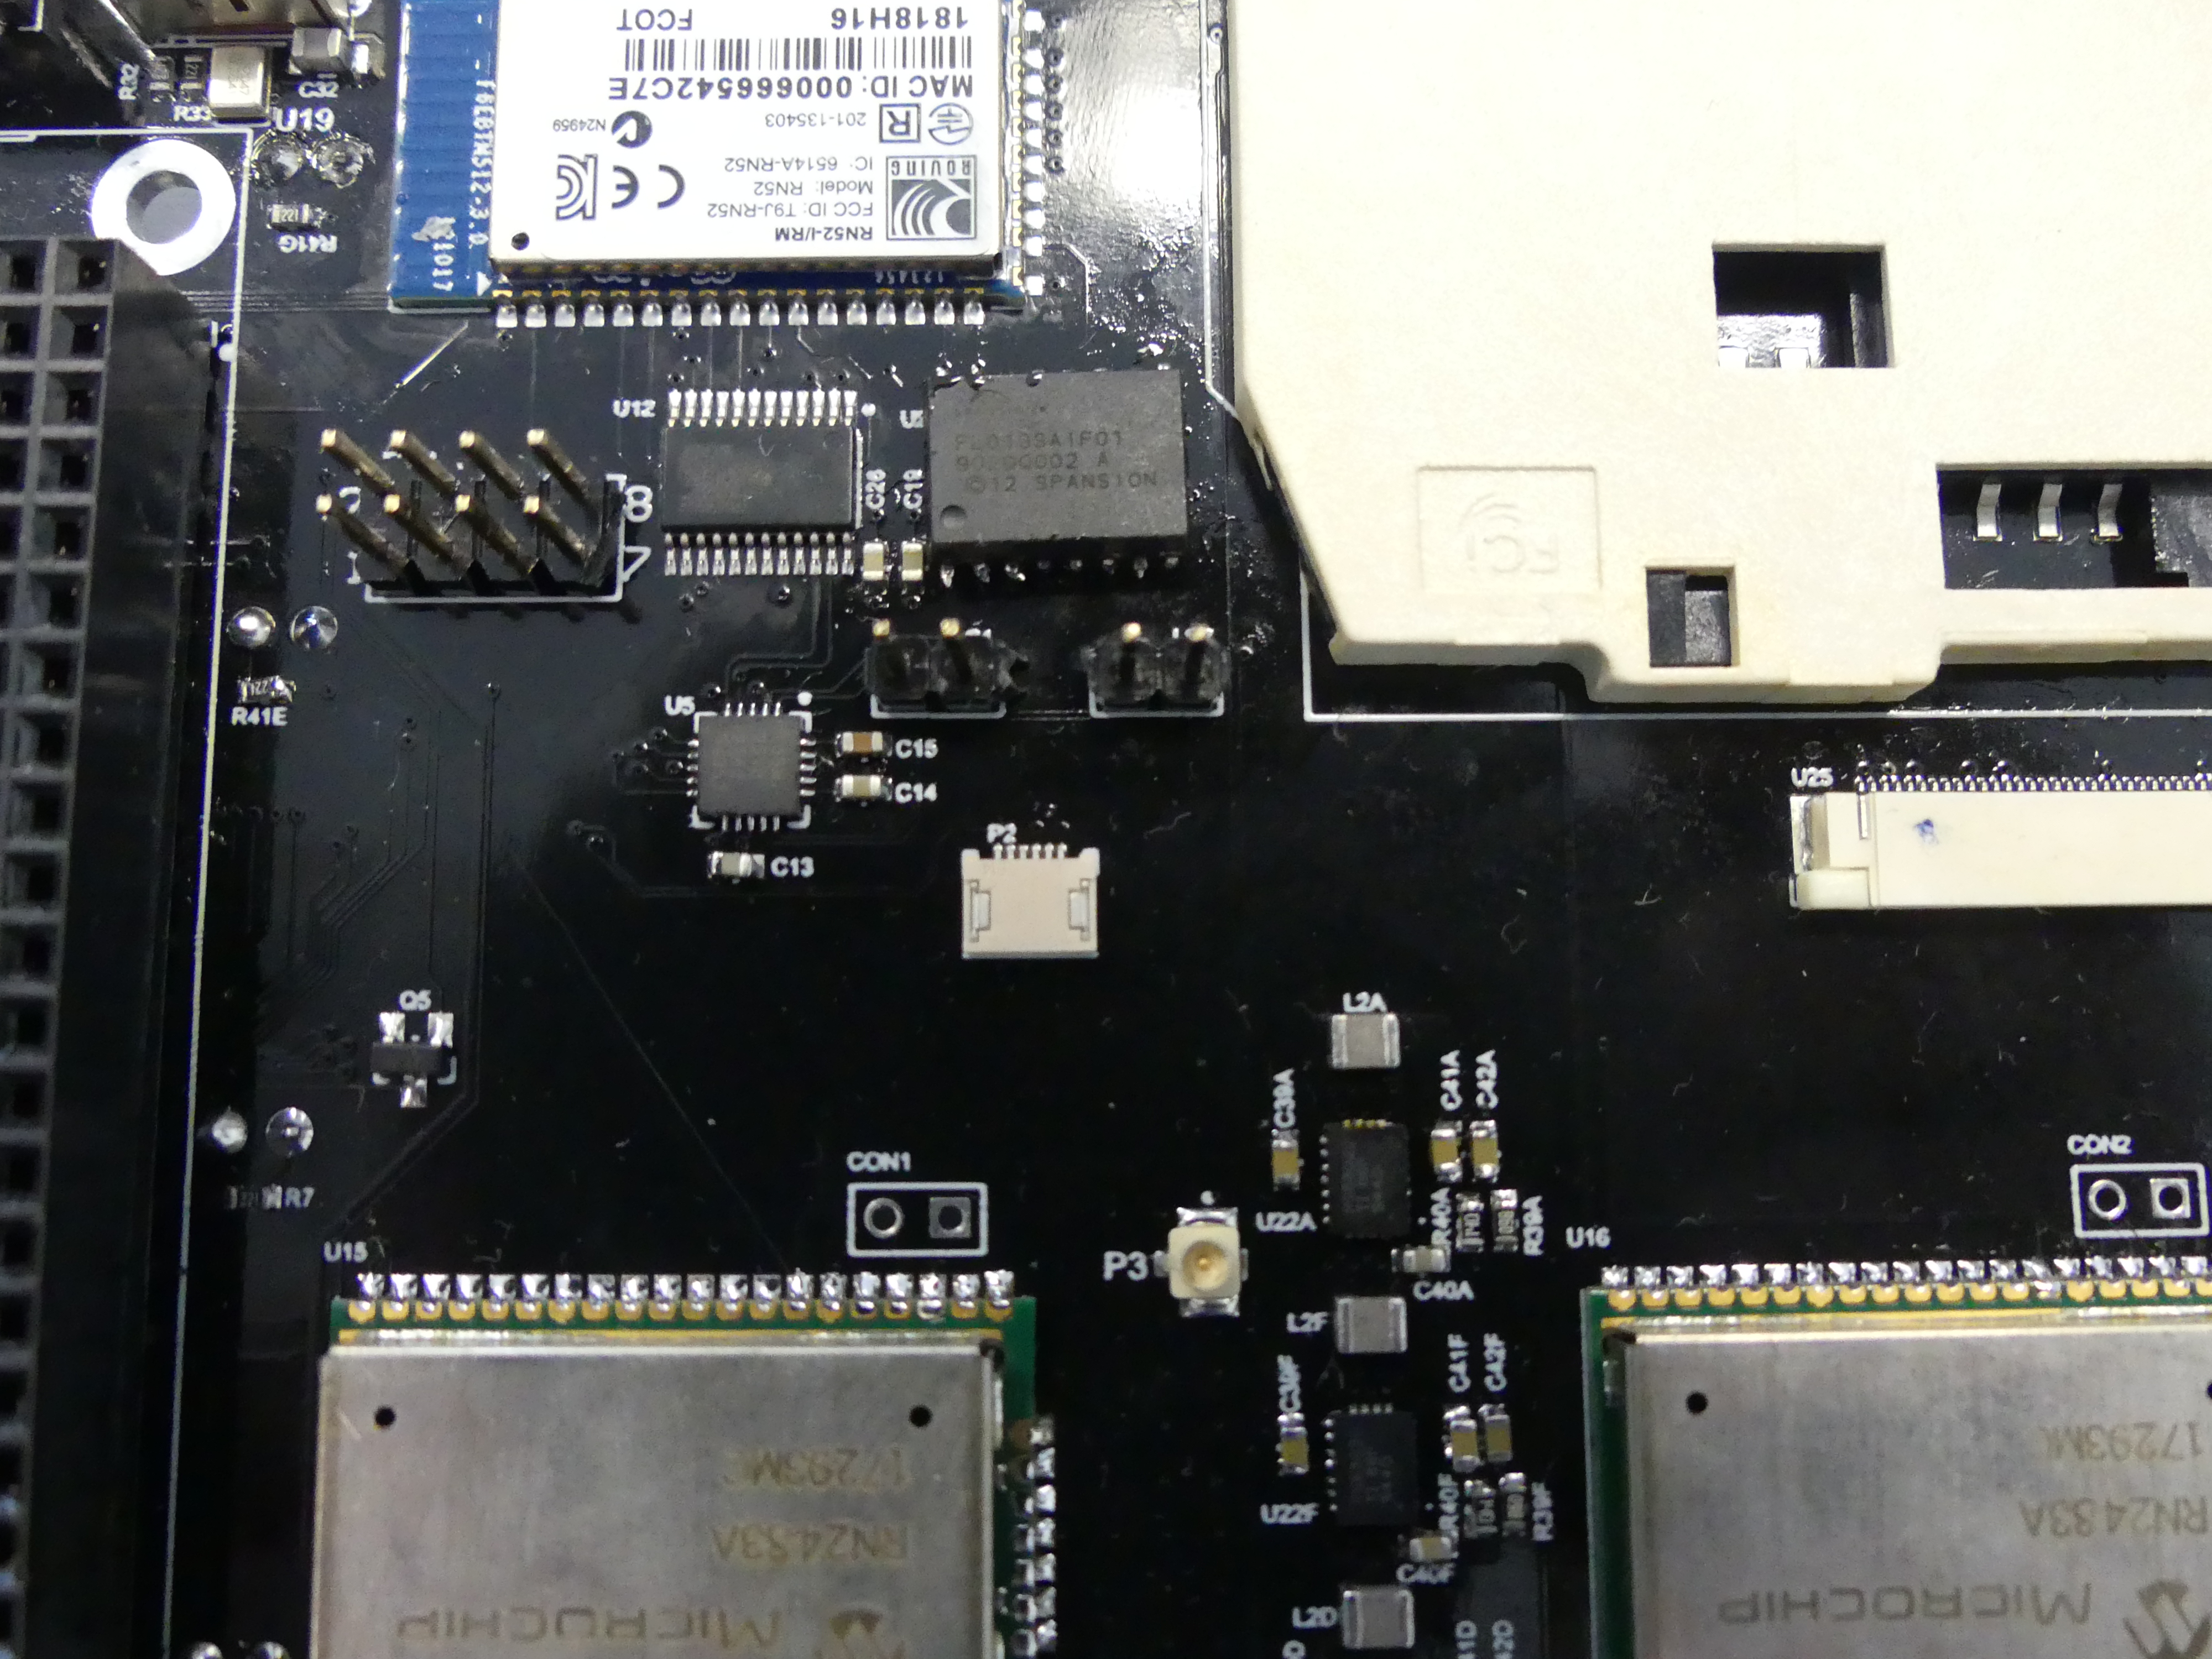
\includegraphics[width=.3\linewidth]{pics/MEGAphone_PCB_r1_P2}
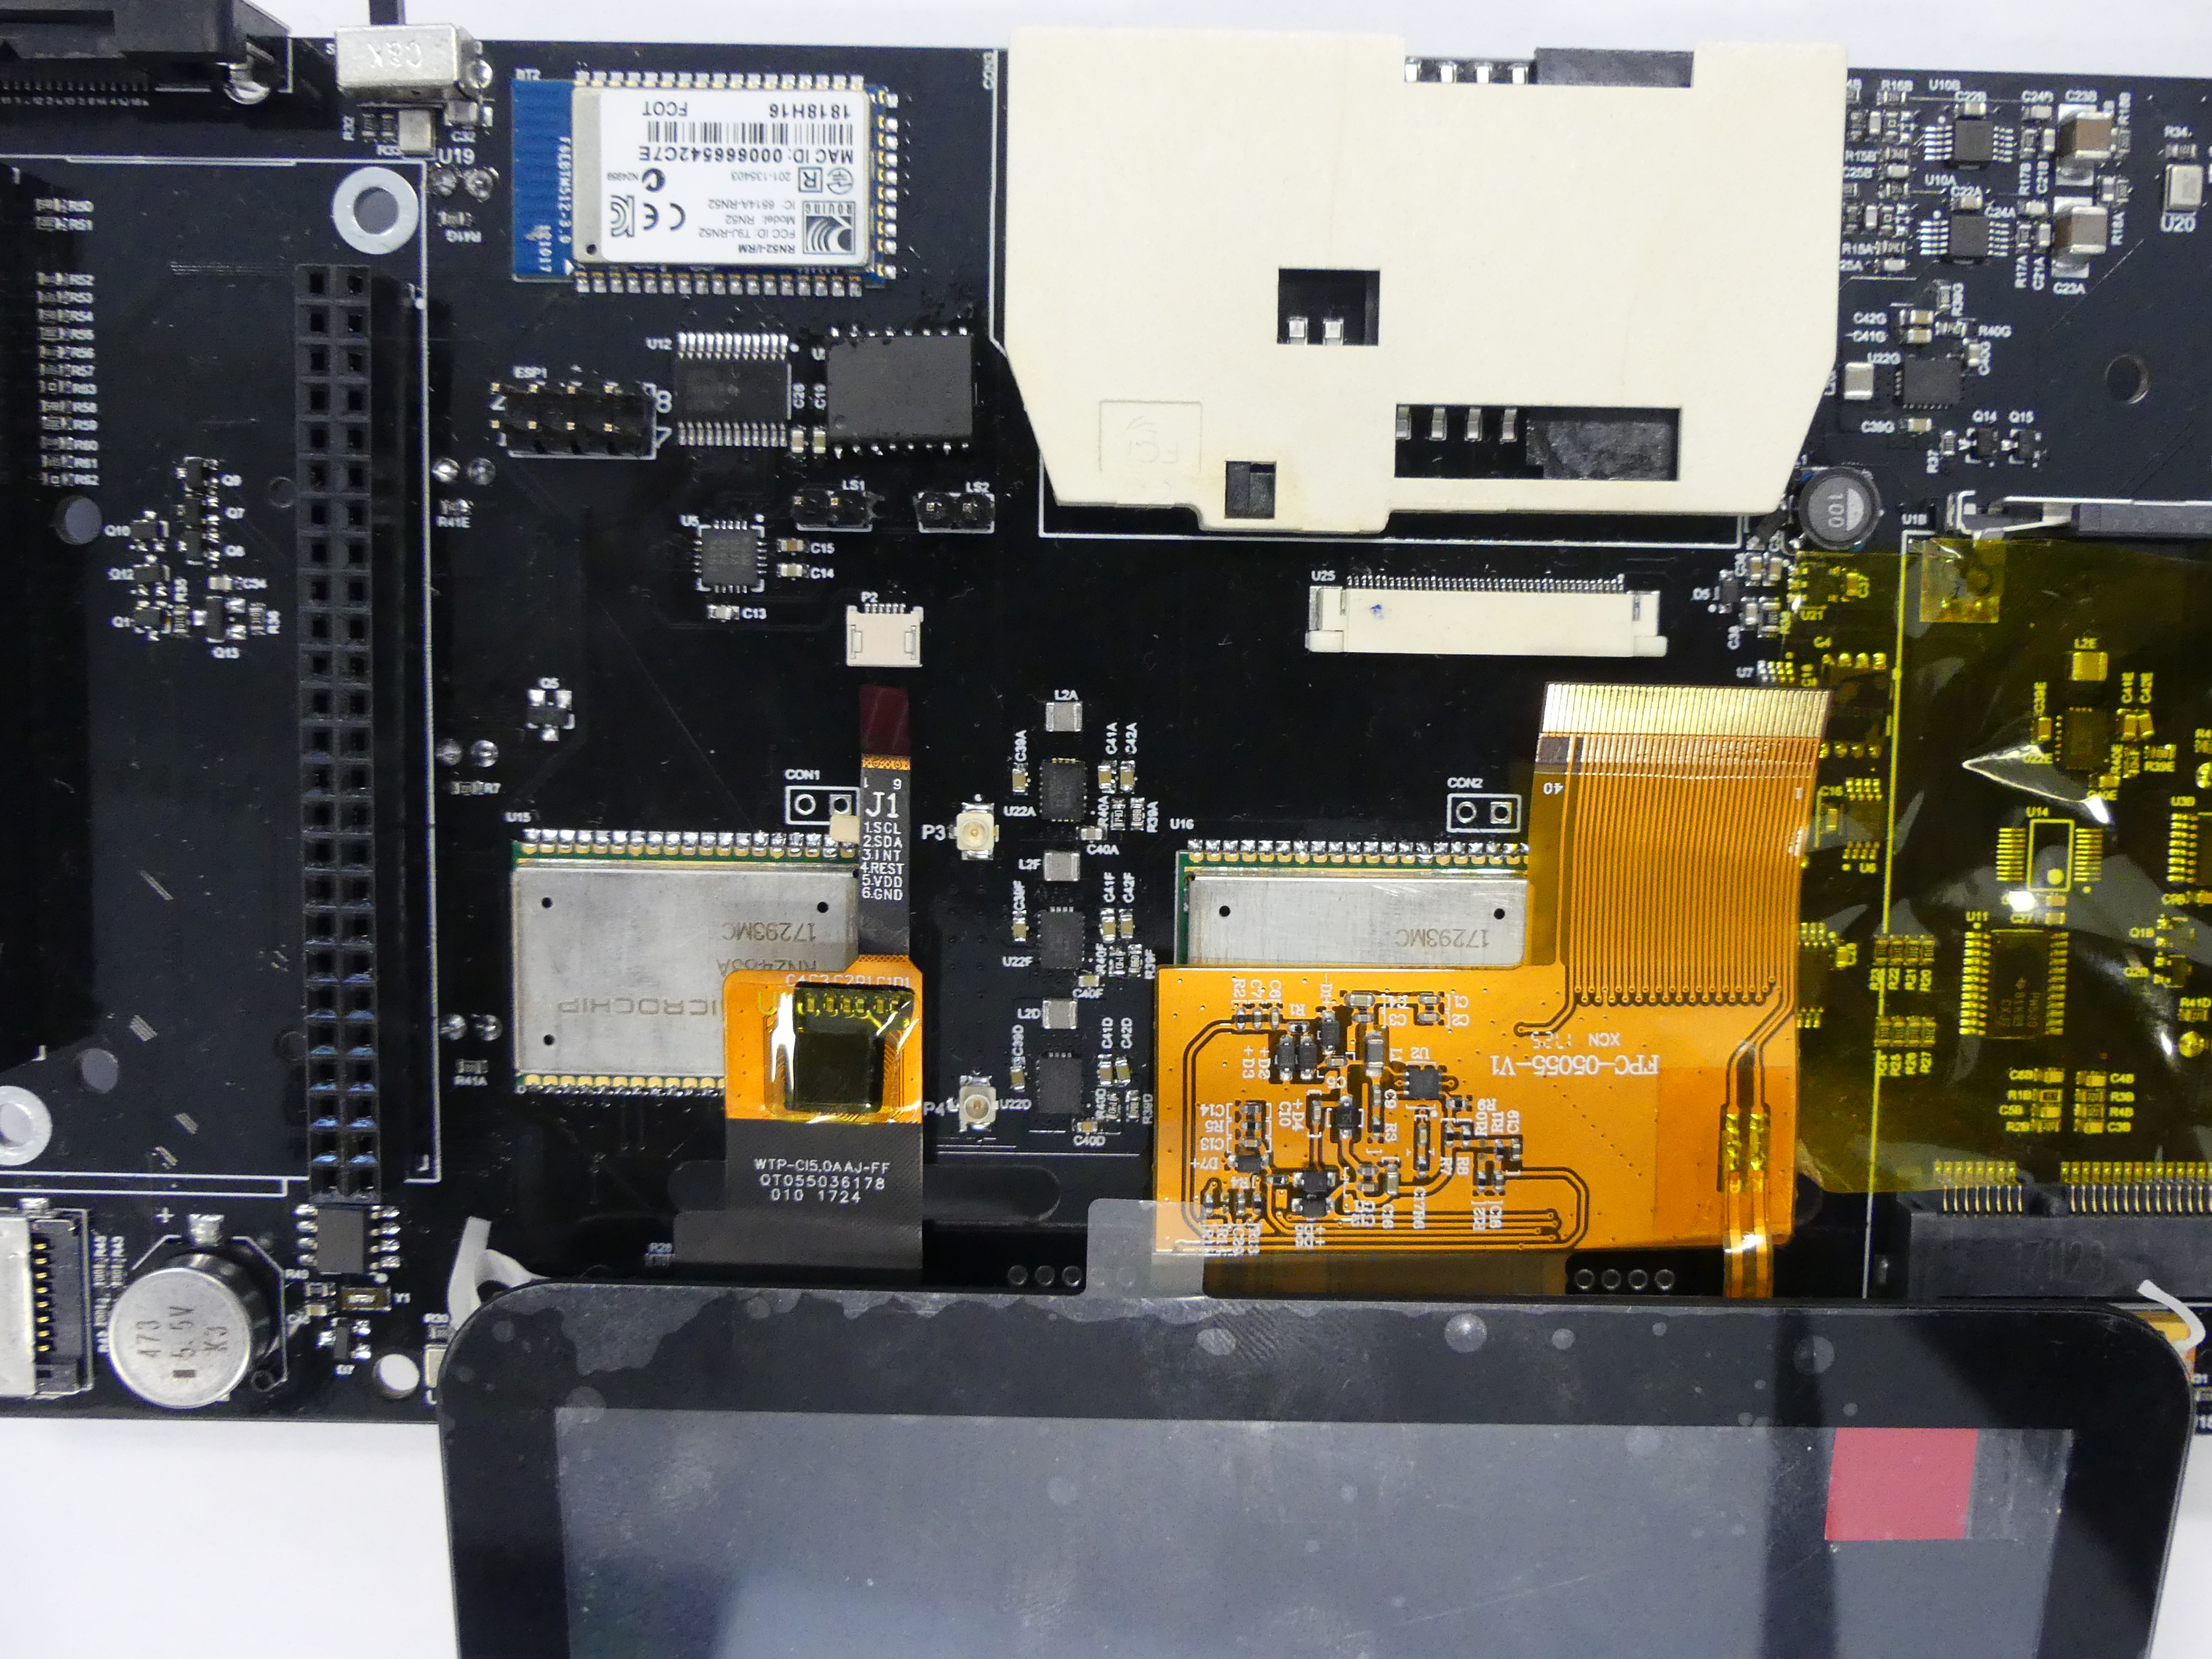
\includegraphics[width=.3\linewidth]{pics/MEGAphone_PCB_r1_U25_P2_ribbon}
\end{center} 
\caption{Close up showing component P2 as well with as the ribbon connector for the screen. P2 needs to be re-positioned. \\}
\label{MEGAphone_PCB_r1_P2}
\end{figure}

\begin{figure} \begin{center}
\includegraphics[width=.3\linewidth]{pics/MEGAphone_PCB_r1_LED1}
\includegraphics[width=.3\linewidth]{pics/MEGAphone_PCB_r1_LED2}
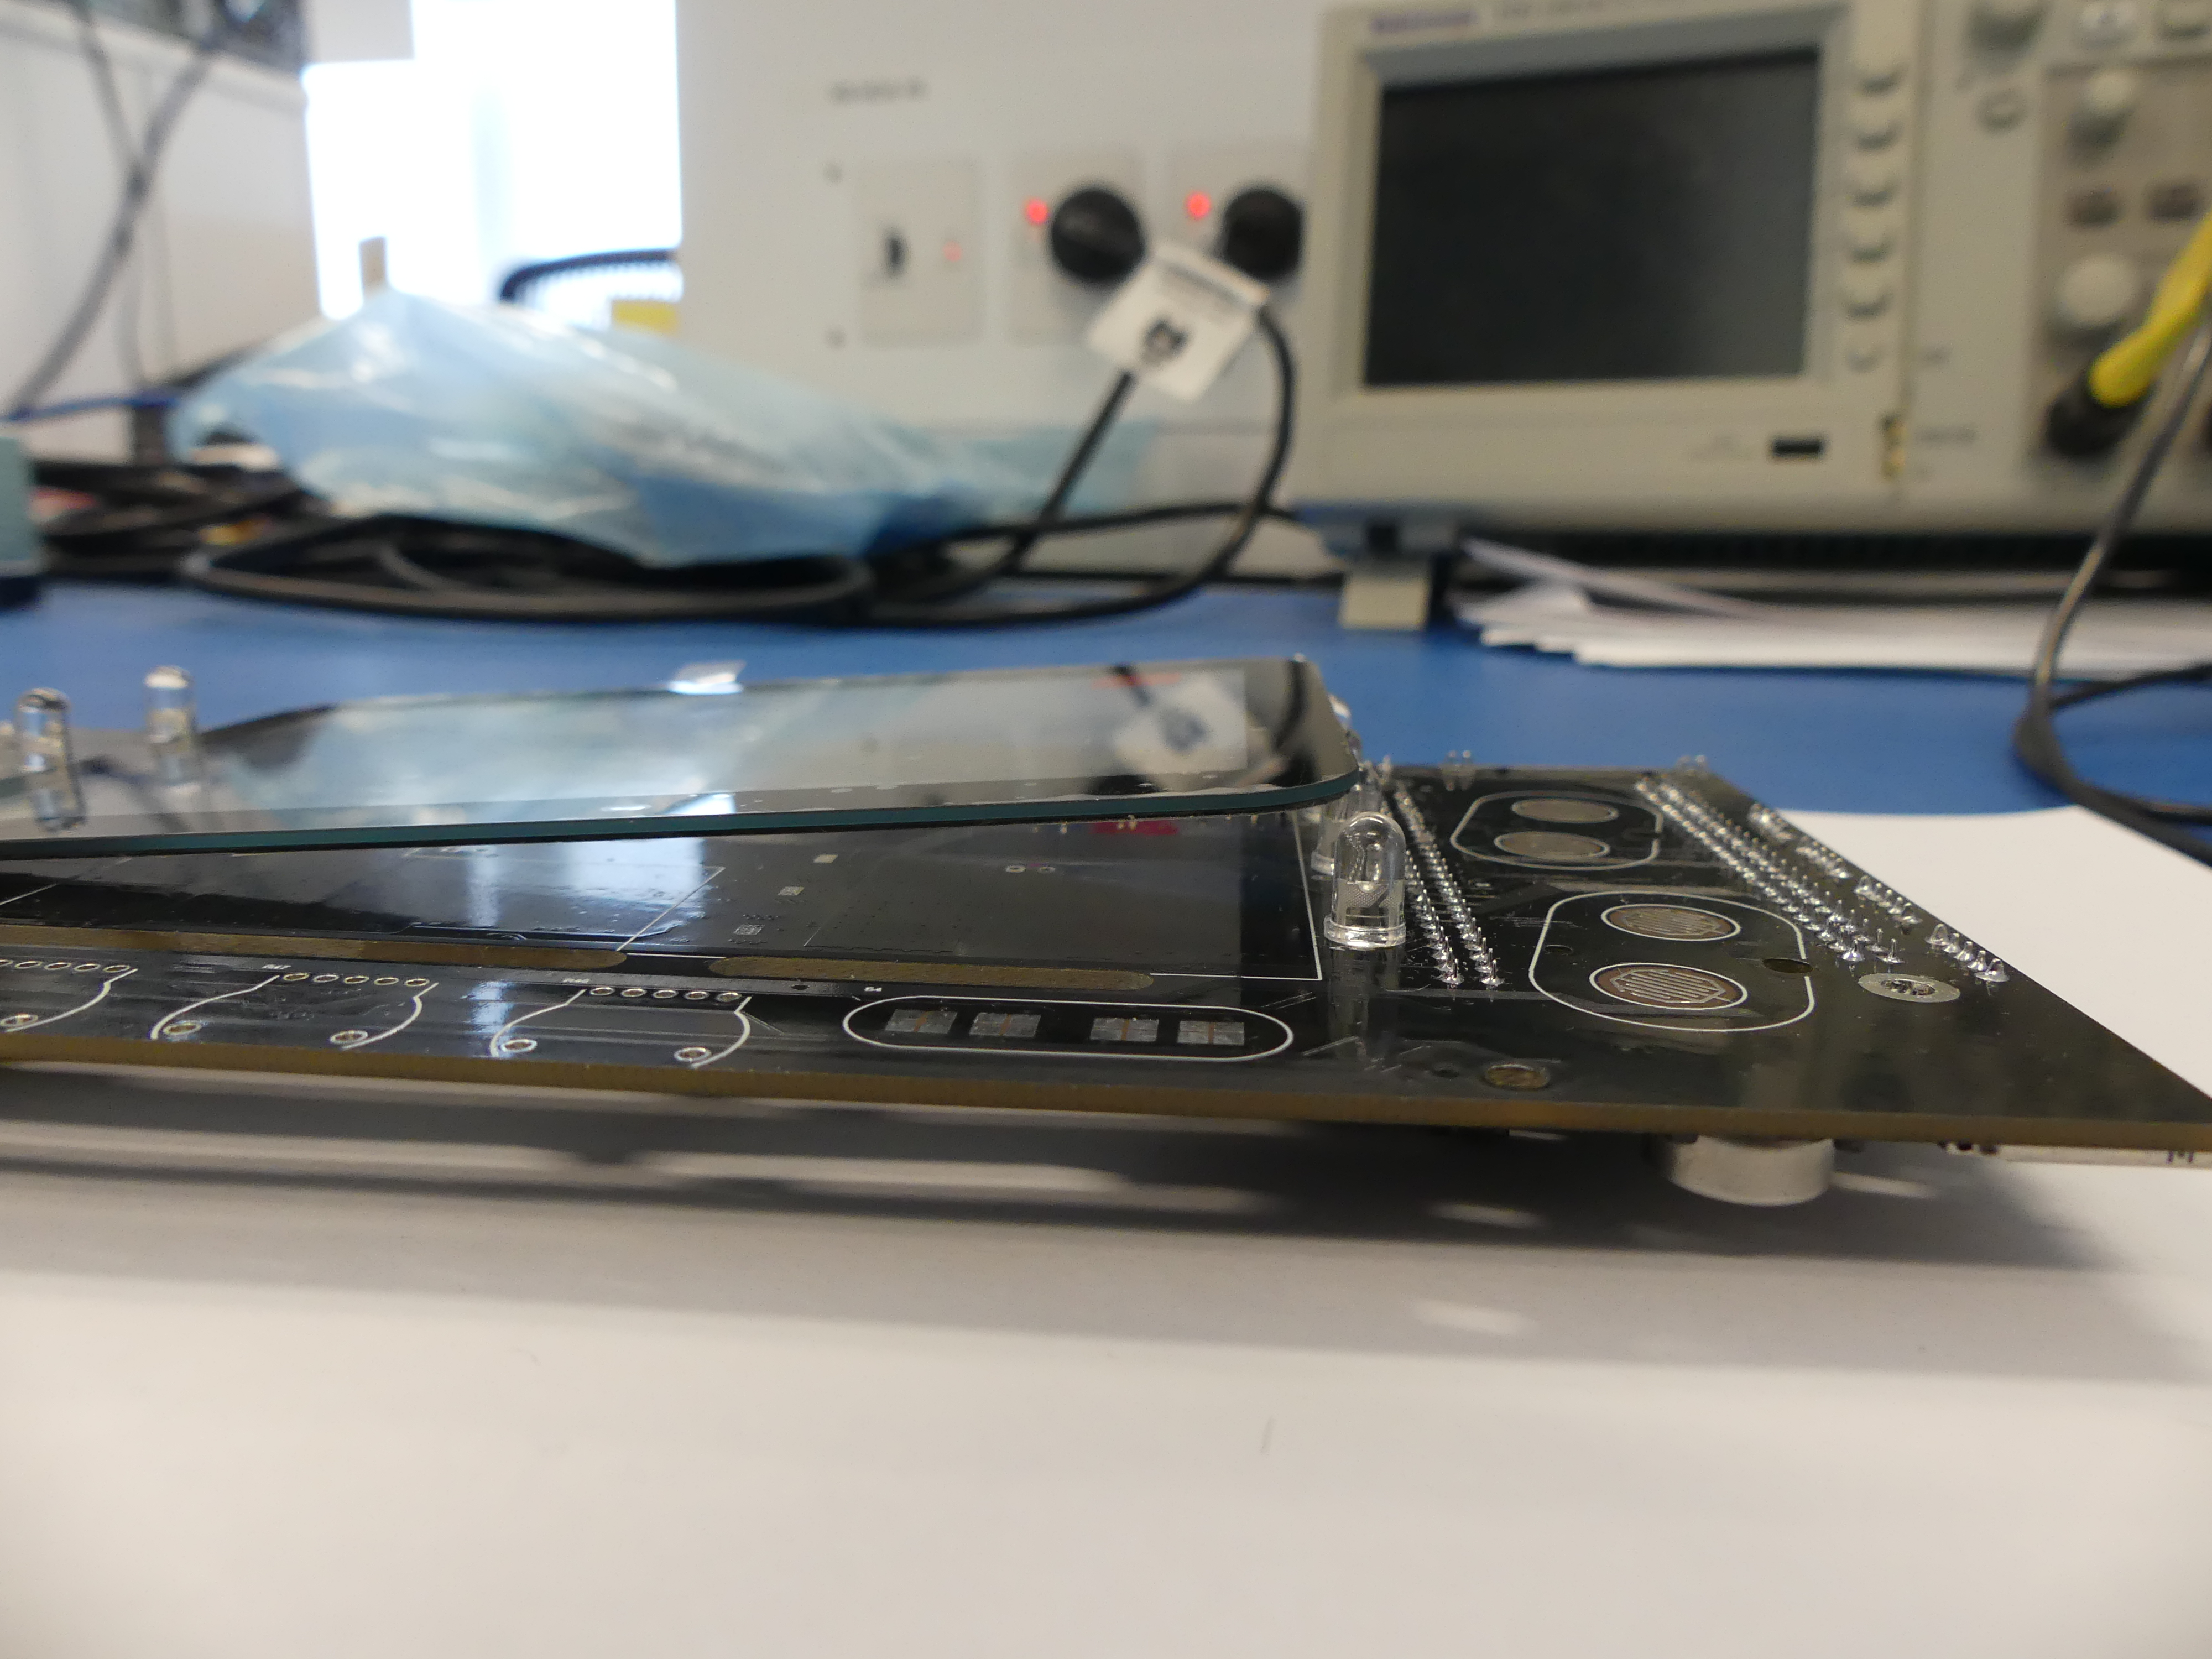
\includegraphics[width=.3\linewidth]{pics/MEGAphone_PCB_r1_LED3}
\end{center} 
\caption{Close up showing position of LED on front face of PCB. Screen cannot fit between them. \\}
\label{MEGAphone_PCB_r1_LED}
\end{figure}

\begin{figure} \begin{center}
\includegraphics[width=.3\linewidth]{pics/MEGAphone_PCB_r1_U9}
\end{center} 
\caption{Close up of U9 which didn't fit its footprint and had to be modified to fit. \\}
\label{MEGAphone_PCB_r1_U9}
\end{figure}

\begin{figure} \begin{center}
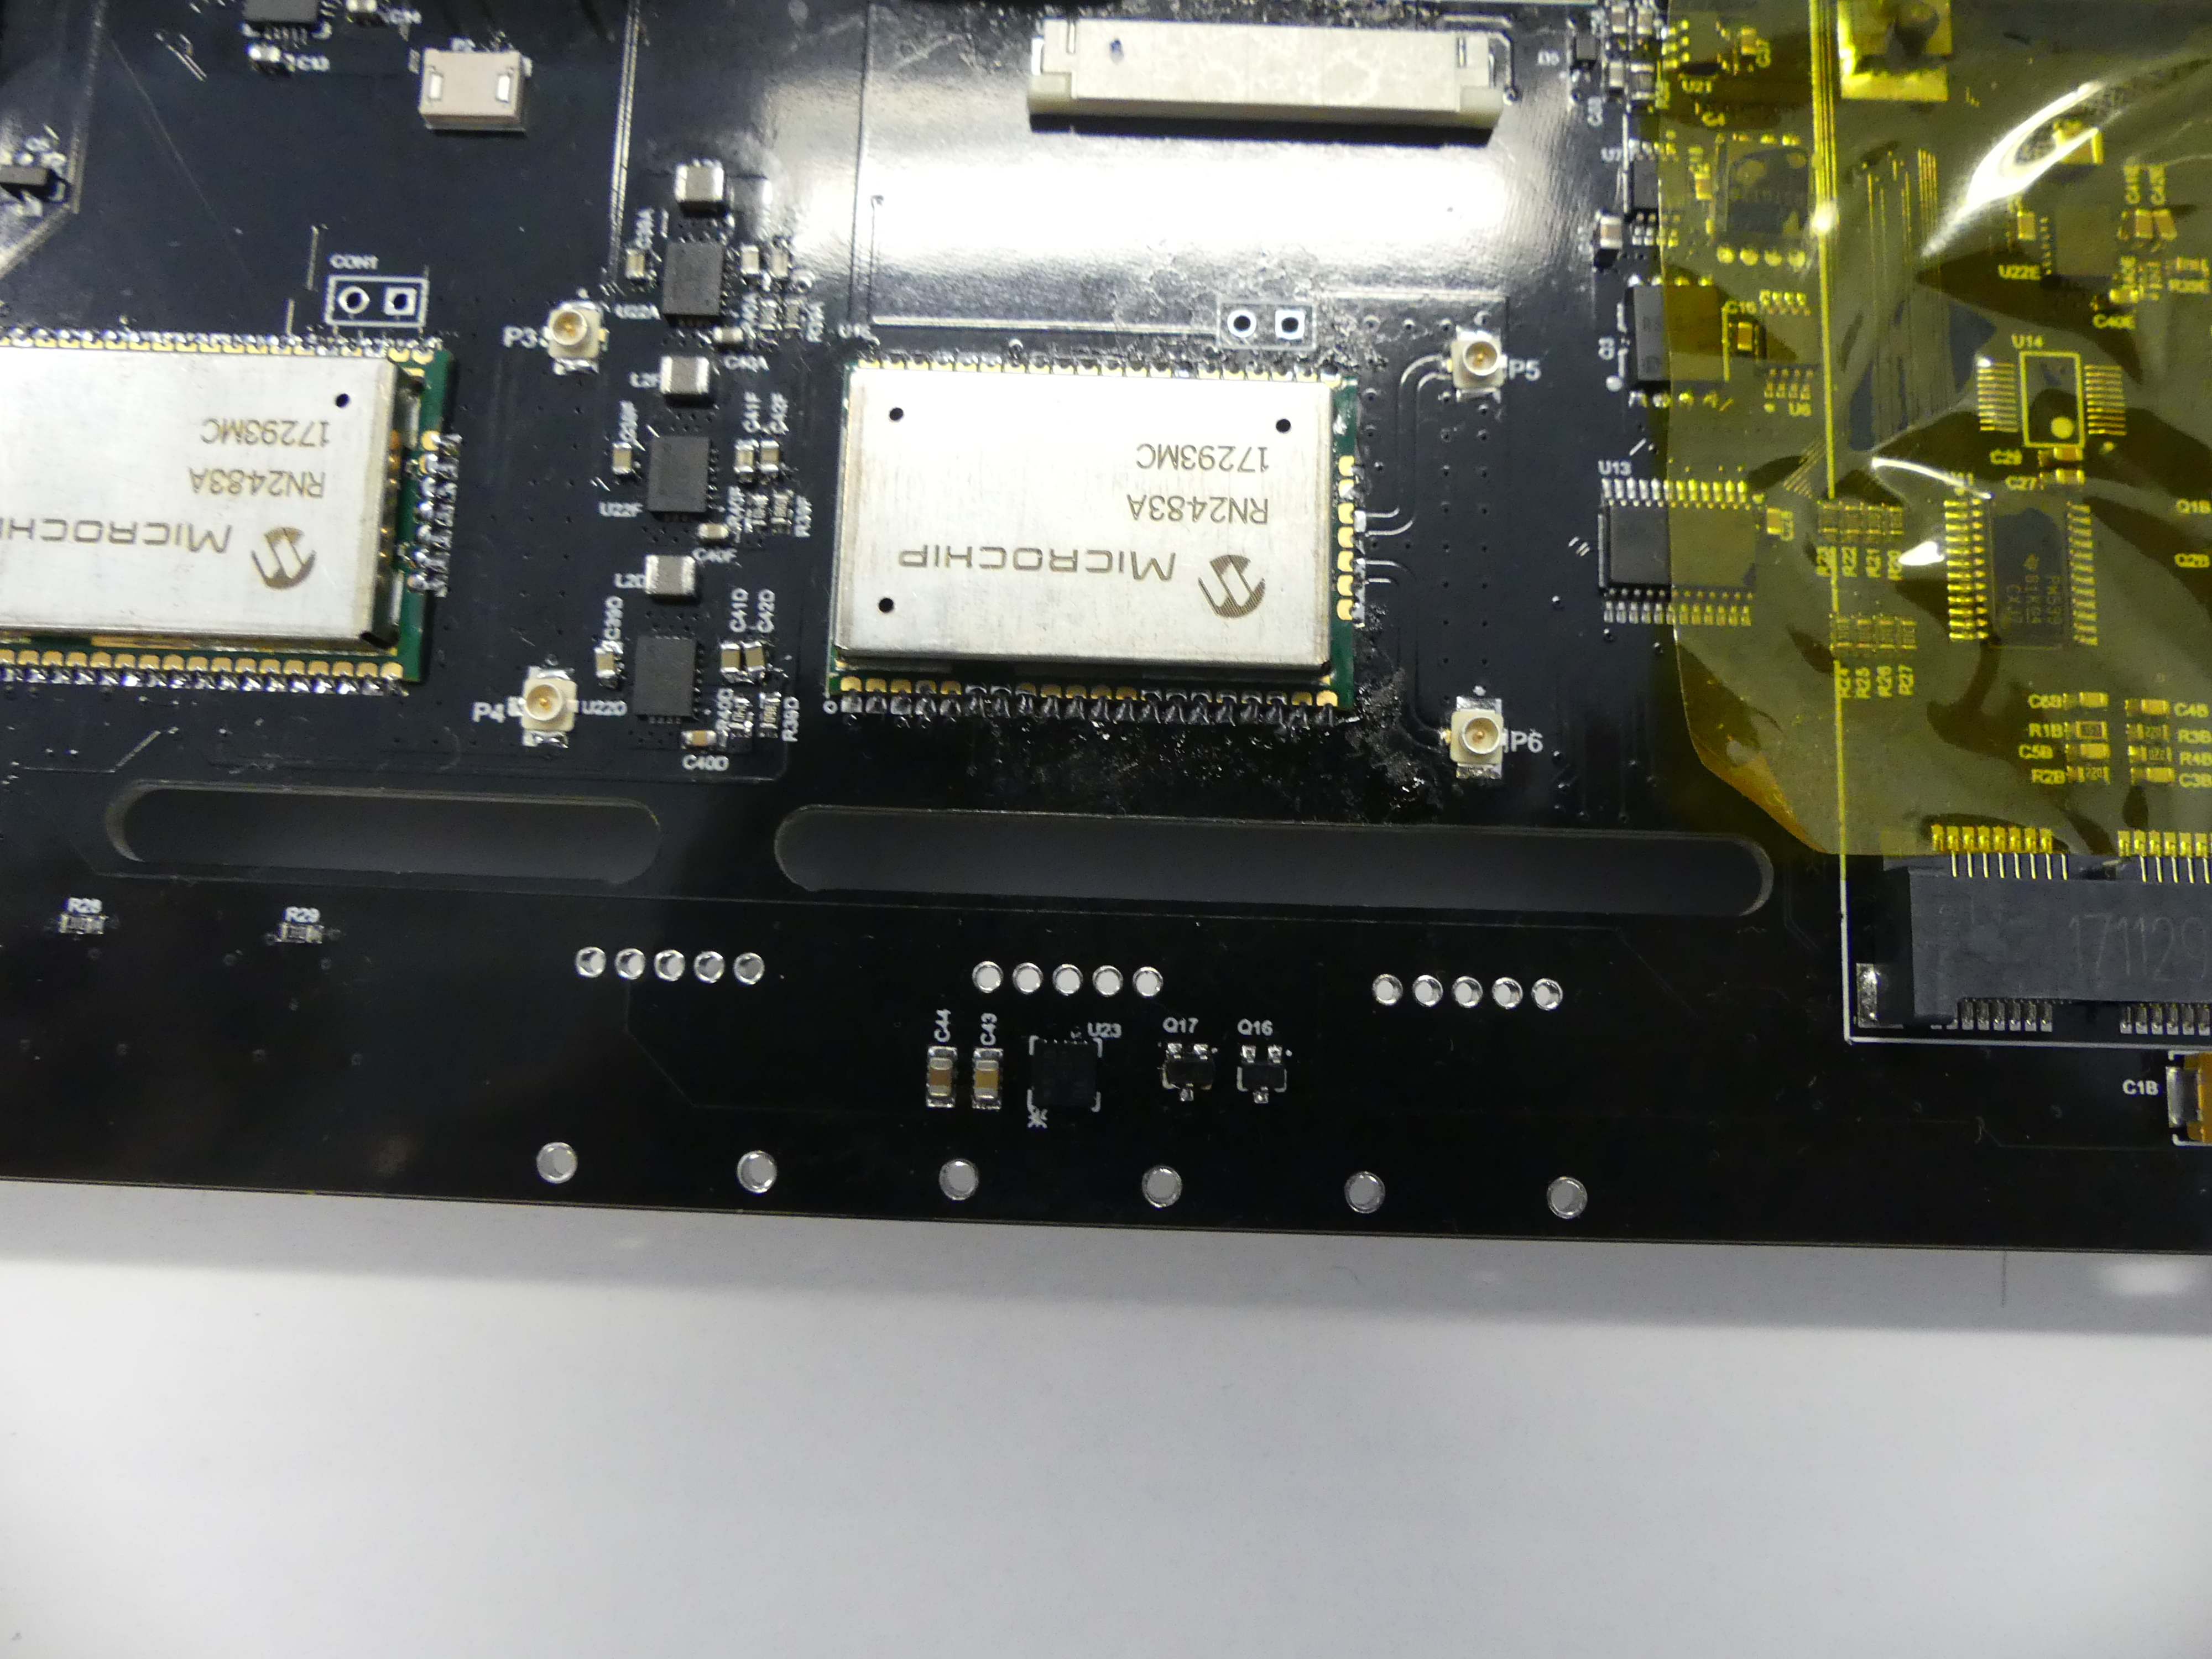
\includegraphics[width=.3\linewidth]{pics/MEGAphone_PCB_r1_R48_R47_R46}
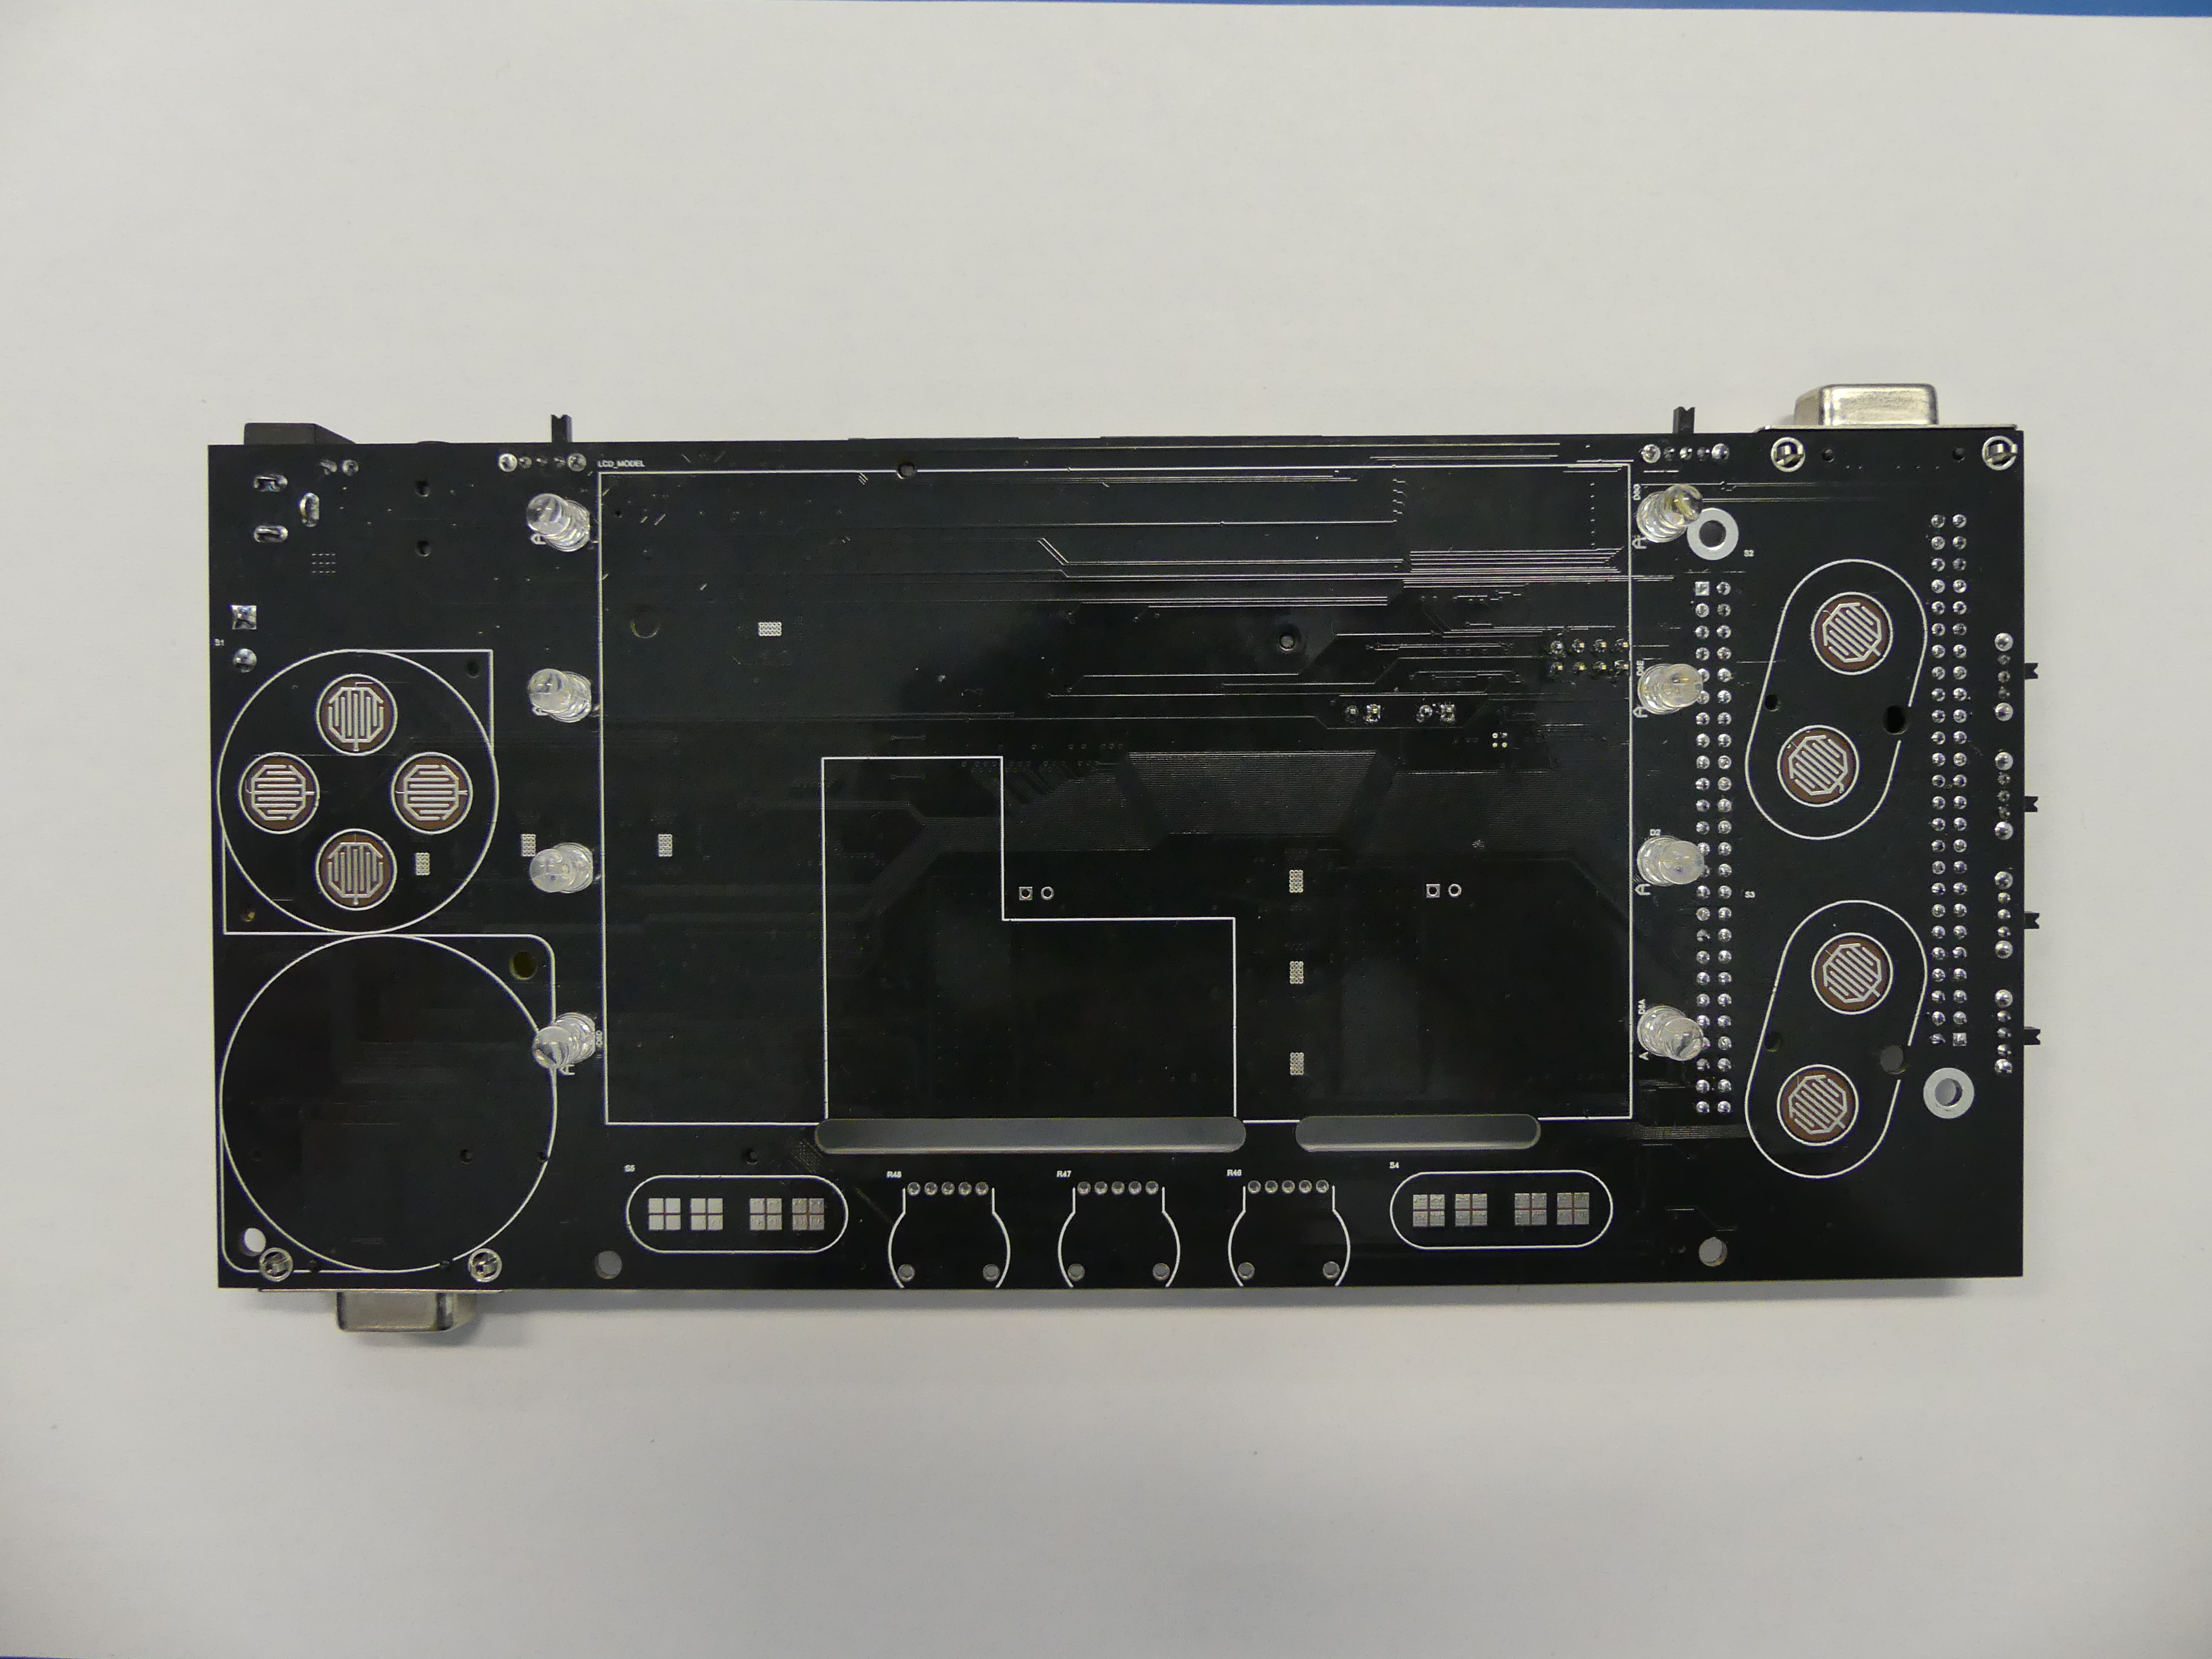
\includegraphics[width=.3\linewidth]{pics/MEGAphone_PCB_r1_populated_front}
\end{center} 
\caption{Close up of missing thumb wheels for volume control, R46, R47 and R48. \\}
\label{MEGAphone_PCB_r1_R49_R48_R47}
\end{figure}

\textbf{Things that need to be tested}
\begin{enumerate}
\item U1A and U1B, might not have enough clearance to fit the cellular modems in place due to components mounted on PCB in this area. 4G modem component to be used to test if it fits. Components within U1A and U1B footprint may need to be relocated if the 4G modem doesn't fit. In particular, the components J1A and J1B may need to be lower profile connectors such as a SIM card connector without the microSD slot above it, which it currently has on both J1A and J1B. Shown in figure \ref{MEGAphone_PCB_r1_U1A_clearance} \\
\end{enumerate}

\begin{figure} \begin{center}
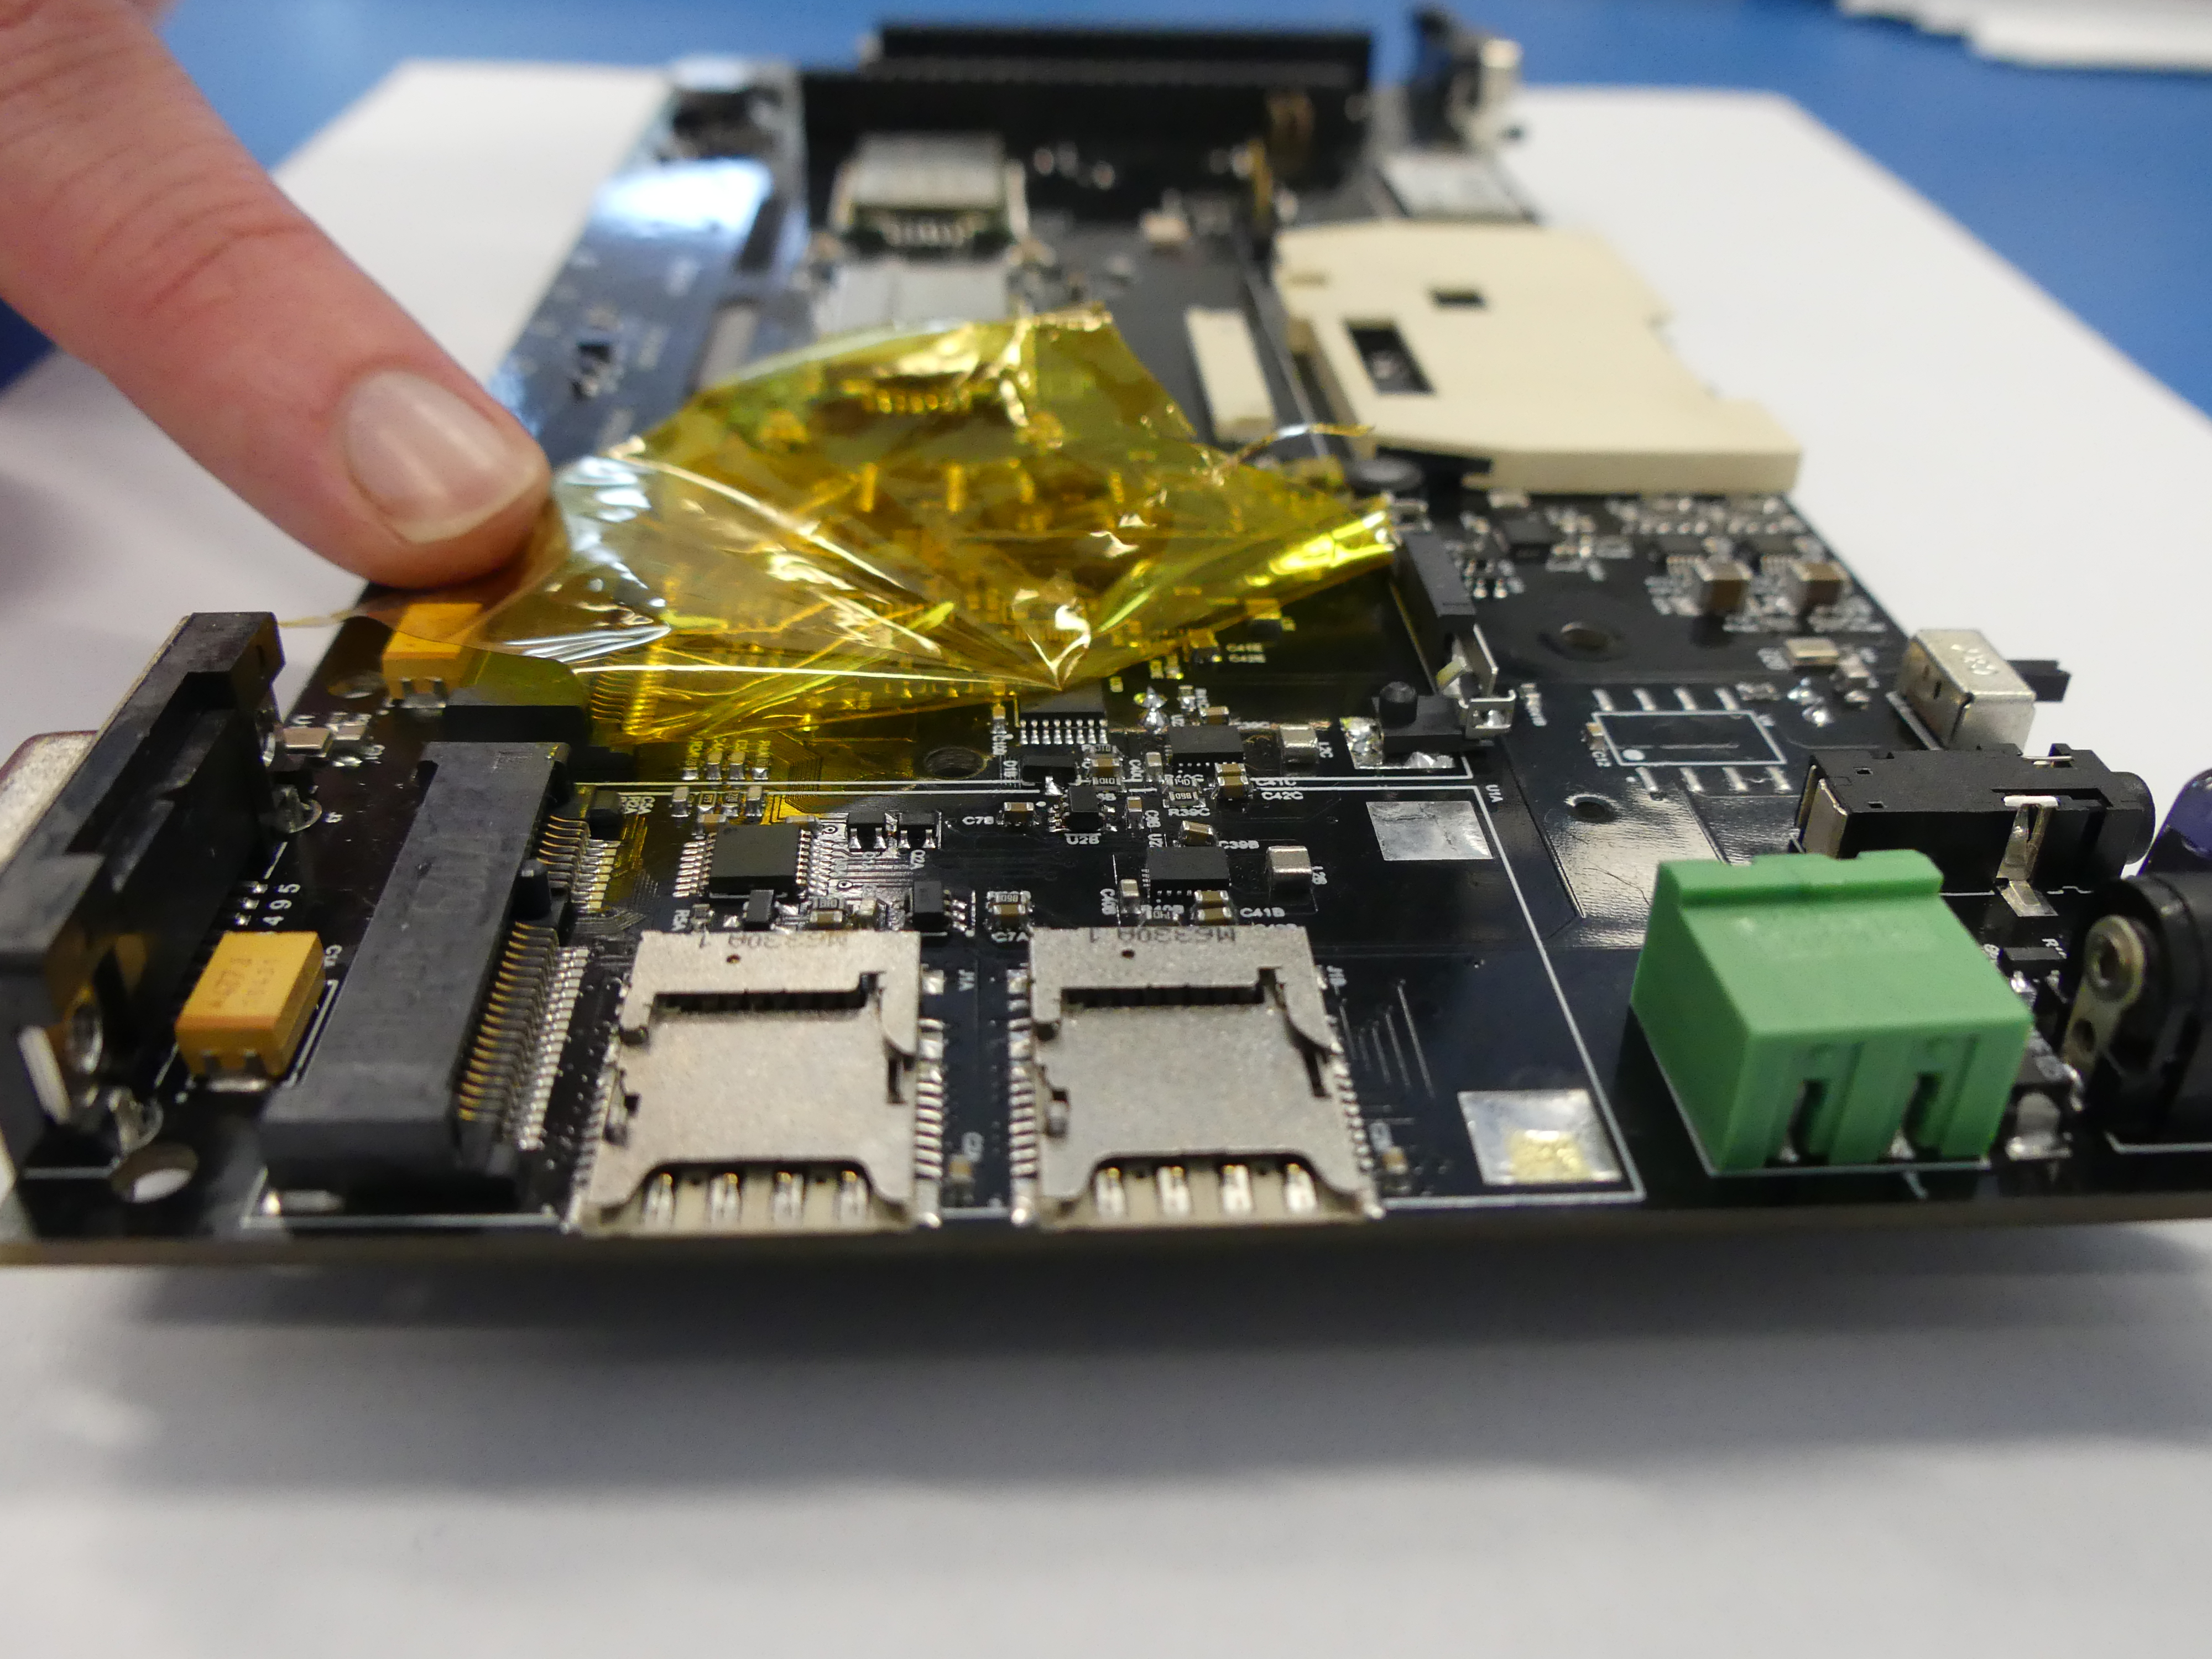
\includegraphics[width=.3\linewidth]{pics/MEGAphone_PCB_r1_U1A_clearance1}
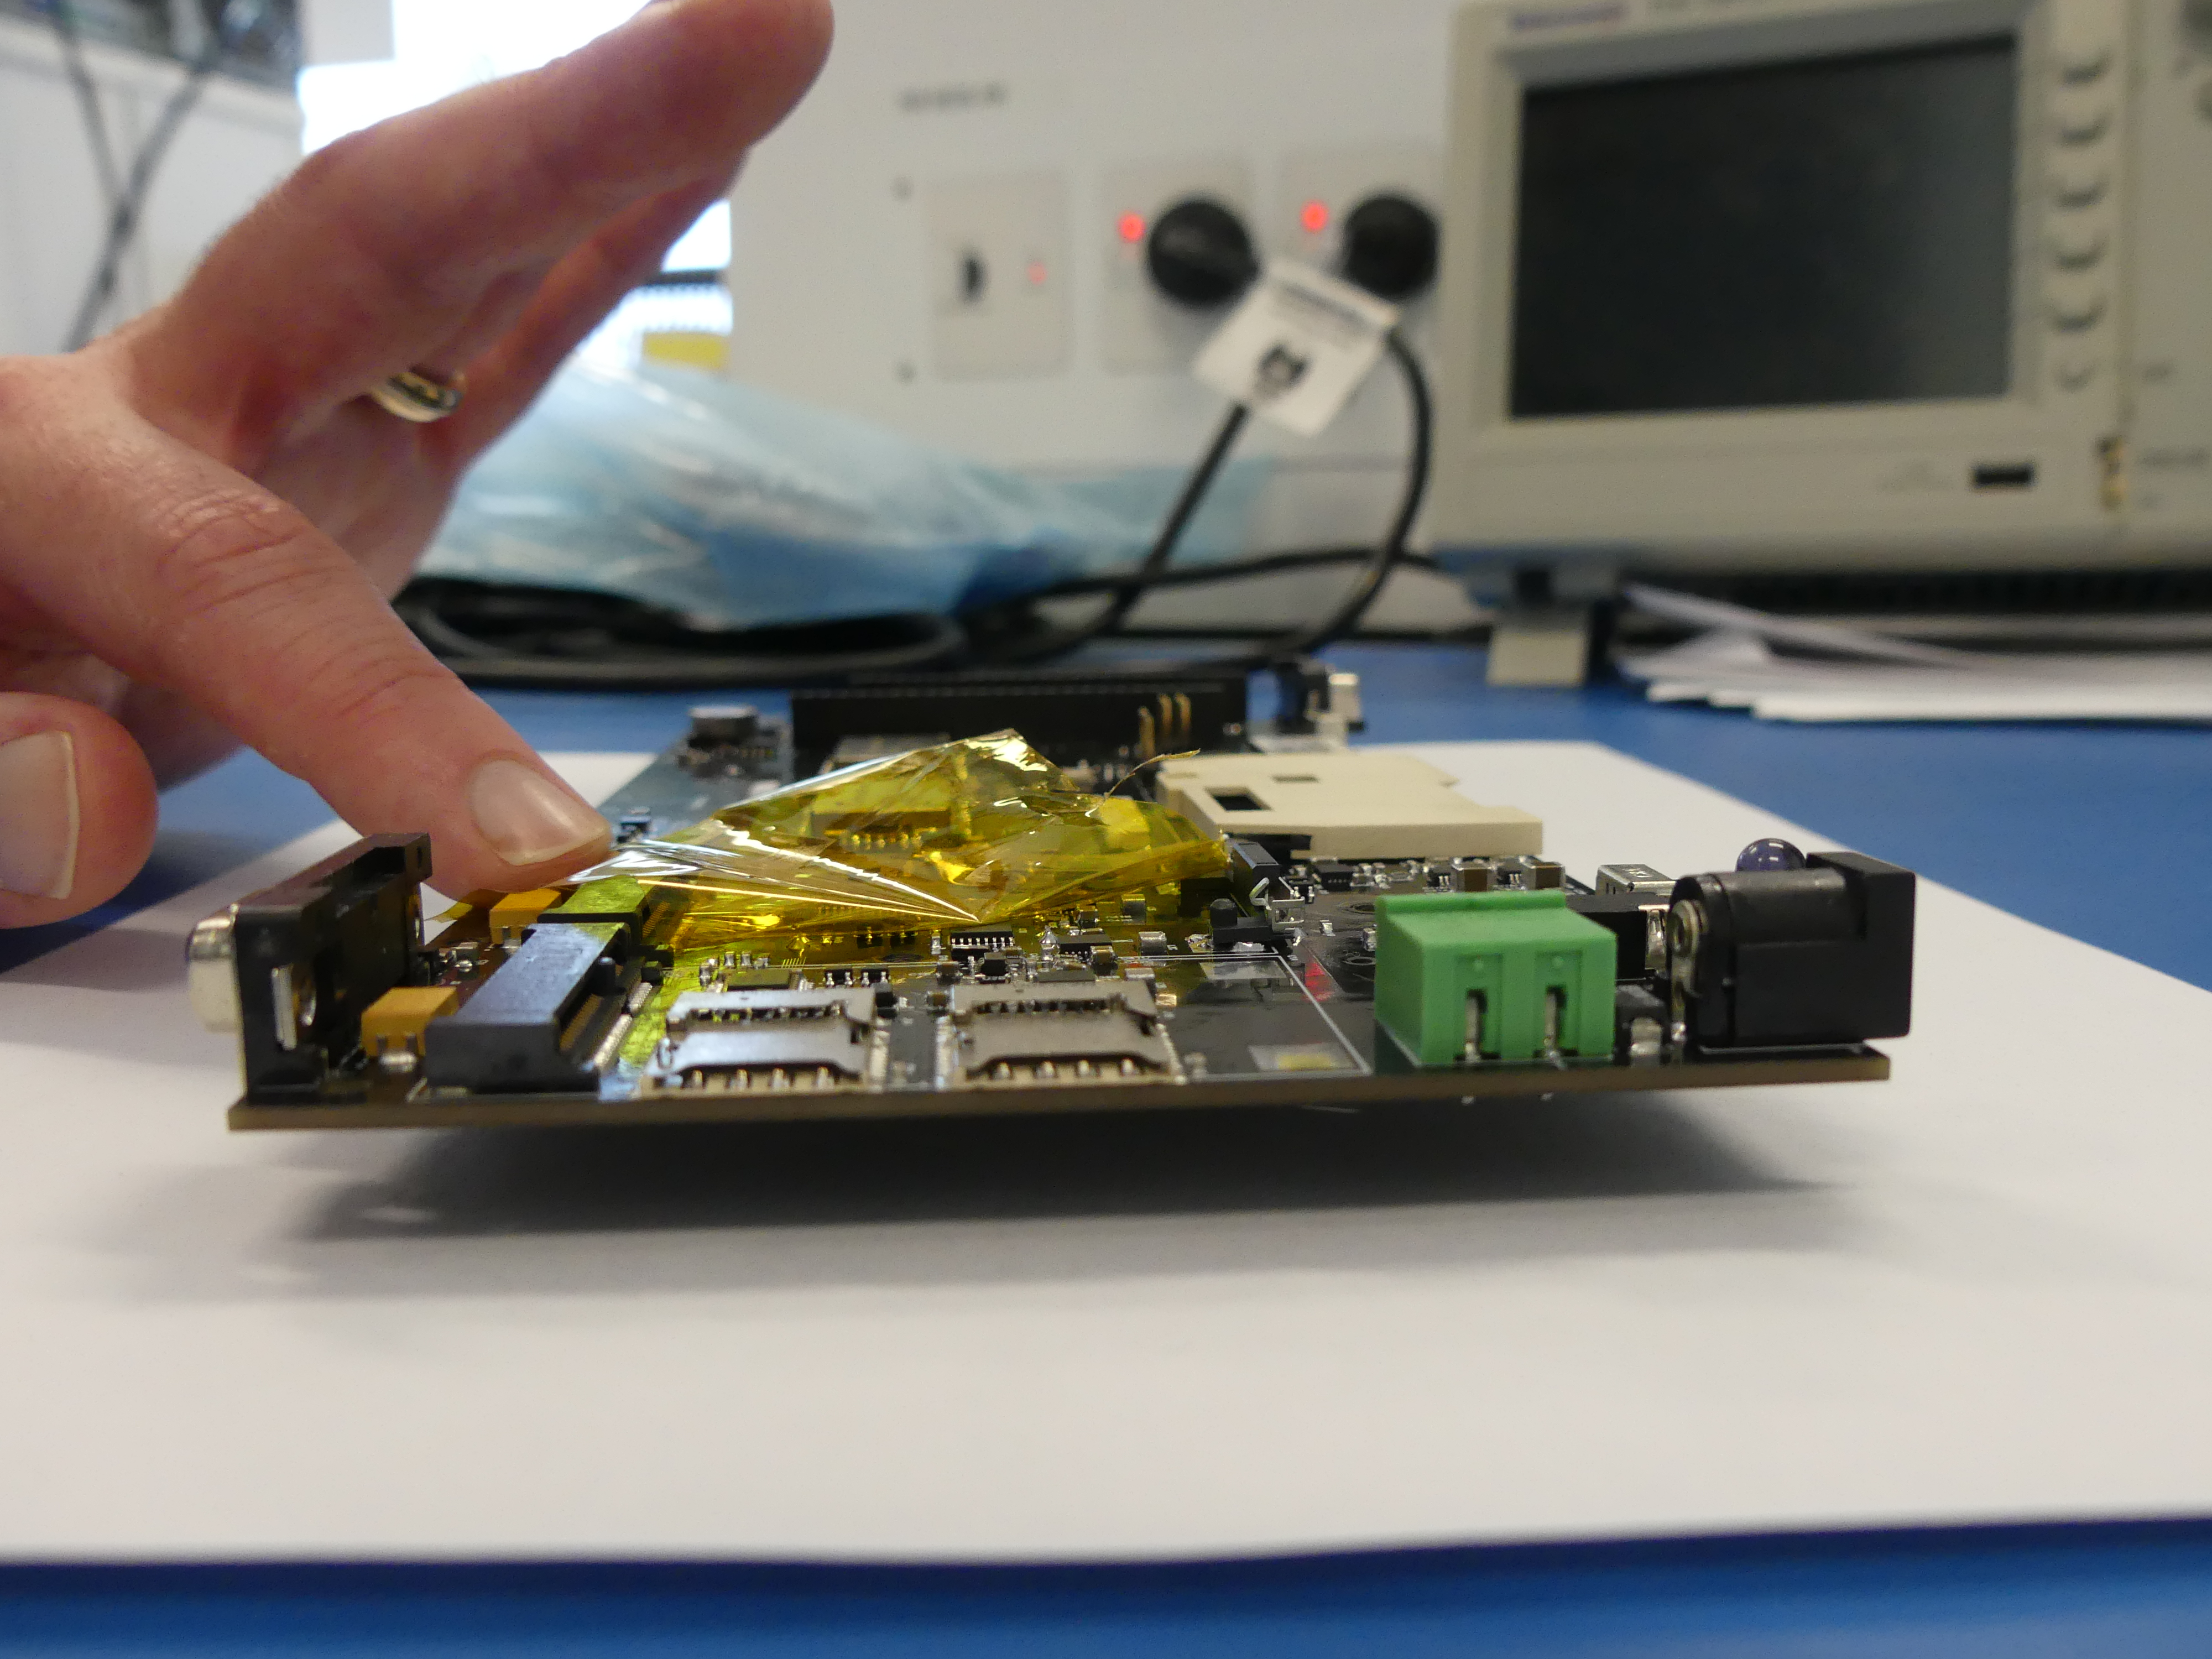
\includegraphics[width=.3\linewidth]{pics/MEGAphone_PCB_r1_U1A_clearance2}
\end{center} 
\caption{Close up of clearance above U1A and U1B footprints, a cellular modem needs to be inserted in this space. \\}
\label{MEGAphone_PCB_r1_U1A_clearance}
\end{figure}


\textbf{Components or functions which cannot be tested currently}
\begin{enumerate}
\item Microphone audio.
\item Thumb wheels for volume control, R48, R47 and R46.
\item 2nd PCIe modem slot, U1A.
\item 2nd SIM card slot, associated with the 2nd modem, U1A, mentioned above.
\item The ribbon cable connections between U25, P2 and the screen cannot be fully tested with the screen in position but a partial test with the screen offset should be possible.
\item Speaker currently not installed but parts and component are present in lab. \\
\end{enumerate}

\textbf{Noteworthy feature}
\begin{enumerate}
\item Installation of insulating tape covering components within the U1A and U1B footprints. This is to provide insulation between conductive part of components and the modem which will be inserted above them, seen in figure \ref{MEGAphone_PCB_r1_U1A_clearance} and \ref{MEGAphone_PCB_r1_U14}. \\
\end{enumerate}


\subsection{Software}



%----------------------------------------------------------------------------------------
%----------------------------------------------------------------------------------------
\section{MEGA65 Desktop Computer Form Factor}
This section looks at the current state of the MEGA65 Desktop form-factor. The Desktop form-factor's physical development is being overseen by M.E.G.A. in Germany. The physical development refers to the electronics hardware, case and keyboard. It still uses the same FPGA-based core, developed by Dr Gardner-Stephens, as the MEGAphone. Following a discussion the Detlef in Germany, who is overseeing the development of the MEGA65 Desktop, the following state of the MEGA65 Desktop hardware was elicited. 

The MEGA65 Desktop is currently in a "pre-series" stage, the machines are roughly 95\% complete and have been created in their current state so they can be tested in a real-life environment. 

\subsection{Hardware}


\subsection{Case}
The current case has had a few modifications from the original design, which was based on the Commodore 65 case. It has a new appearance with a original case design which has been described as "cleaner". The new case also has some major changes around the port at the back of the computer and some minor changes to the trapdoor on the bottom as well as some additions for ventilation. These design changes to the new case where carried out by Hintsteiner in Austria.

The MEGA65 Desktop is planned for a pre-production run of 20 machines using the new case design. This run will use vacuum moulds for the cases to reduce costs but the vacuum mould process has some drawbacks: 
\begin{enumerate}
\item The mould will only only be bale to create 20 cases before it has to be replaced.
\item The colour of the plastic forming the case slightly changes between cases.
\item Some parts of the case need to be manually fixed after the vacuum mould adding costs and the need to paint sections of the case.
\end{enumerate}

*PIC OF NEW CASE TO COME FROM DETLEF*

\subsection{Keyboard}
The keyboard for the MEGA65 Desktop is being produced by GMK, a German company. It features Cherry MX mechanical switches and 2 embedded metal plates, intended to provide very high stability. There are 2 LEDs for the lock keys, capslock and numlock and 4 RGB LEDs for power and floppy activity indicators, these are all powered by a custom-made communication bus. The keyboard also has a CPLD-based controller in place of the more widely used ARM7 microcontroller, this was done intentional to avoid "having more intelligence inside the keyboard than inside the computer".

Detlef has ordered 25 keyboards for the pre-production run, this was intentionally more than the 20 cases being produced, as mentioned above. It will provide for 5 case-less machines to use as spare-parts. It is expected that the keyboards will be in a finished state and require no more design work 

\subsection{PCB}
The PCB provides the interface between the FPGA architecture and the physical circuitry required for such features as the LEDs, I/O ports, speakers and keyboard. The design of the PCB for the MEGA65 Desktop version is being carried out by Antii Lukats at Trenz Elektronik. Currently Lukats is working on the 'r2' version of the PCB and it should be finished in early April, 2019. From there a pre-production run of 25 will be manufactured and then populated with components, before being send to Detlef. 

During the design of the PCB, a challenge arose from the need to combine modern components with much older components such as the floppy disk connector and the 9-pin joystick port. This required a larger number of different voltage levels to power the components than a purely modern component machine. 

\subsection{Other Components}
To make a finished product the MEGA65 will need more than the computer its self, there also needs to be considerations and preparations made for such things as the box, manual, silica gel for packing, warning and warranty paperwork and CE certification paperwork. To complete the computer itself also requires some extra items such as serial number stickers, warranty seals/stickers, type signs, power supply units, screws, SD card, floppy drives and cables. 
%Chapter 6 - Re-evaluating the MEGA65 project against known risks
% 	Did the MEGA65 project reduce its risk after 10 months?

\chapter{Risk evaluation of the MEGA65 project in May 2019}
\label{Chapter6}
After a 10 month period, the MEGA65 project was re-evaluated against the risks identified in chapter \ref{Chapter3}. This period of time gave the project sufficient time to act on the suggestions given at the end of chapter \ref{Chapter5}. By re-evaluating the MEGA65 project and comparing the result with the evaluation from July 2019, it is hoped that a conclusion can be drawn on whether the MEGA65 project reduced its risk exposure or not. 
%----------------------------------------------------------------------------------------
%----------------------------------------------------------------------------------------

\section{Laws and regulations}
The MEGA65 project has undertaken some research into the laws and regulation which need to be upheld in some of their key markets in which they expect to operate. With the knowledge gained from the research, the uncertainty in the relevant laws and regulations is reduced, as such the overall risk to the project is reduced. Not every market was researched, and the unknown markets still expose the project to risk if the MEGA65 where to be sold within it. The MEGA65 project is rated as having an unlikely chance of occurring and if it causing a marginal level of potential damage. \\

Likelihood - Unlikely \\
Potential damage - Marginal \\
Risk - Low \\


\section{Sourcing old components}
During the interim 10 months the MEGA65 project purchased 700 3.5" floppy disk drives and has them in storage in Germany. These disk drives are to be used as components during the assembly of the MEGA65 desktop version. This action of purchasing a large surplus of stock allows the MEGA65 project to avoid this risk in the medium term. When the stock runs out the risk will increase, as such the risk is largely tied to the MEGA65's popularity and sales volume. If the MEGA65 becomes hugely popular then this risk could increase dramatically. If the MEGA65 sells as expected by the MEGA65 project team, then 700 drives will be sufficient for the medium to long term. The potential damage the MEGA65 project is rated as marginal and the chance of it occurring possible. \\

Likelihood - Possible \\
Potential damage - Marginal \\
Risk - Moderate \\


\section{Use of 3rd party intellectual property}
The MEGA65 project has enacted some of the suggestions from chapter \ref{Chapter5}. The steps undertaken in the identified risk areas are discussed below.

\subsection{Commodore logo}
The MEGA65 team decided to use their own design for the logo on the Commodore keyboard key. They have created and used the design for the pre-production run of the desktop form factor. This new design should completely remove the potential for this risk to effect the MEGA65 project.

\subsection{Commodore 64 character set}
The MEGA65 have decided to replace the Commodore character set with one they have created themselves from other freely available character sets and their own work. By removing the Commodore character set the risk eliminated. 

\subsection{Commodore BASIC ROM and kernel ROM}
The MEGA65 team have decided to created their own BASIC and kernel ROMs. This reimplementation is currently under way and can provide basic functionality at this stage. By removing the Commodore ROMs from the MEGA65, the risk is entirely eliminated. \\

Likelihood - Rare \\
Possible Damage - Negligible \\
Risk - Low \\


\section{Open-source business}
The MEGA65 team have not trademarked the MEGA65 name and are operating under the assumption that the MEGA65 will not be hugely popular. The MEGA65 team have been made aware of the strategies listed in chapter \ref{Chapter5}, these strategies are only sensible if the MEGA65 becomes hugely popular and cannot be enacted to much benefit before. Because the MEGA65 team is aware of these strategies the MEGA65 project's potential damage and chance of occurring are both lowered compared to July 2018. \\

Likelihood - Unlikely \\
Possible Damage - Moderate \\  
Risk - Low \\

\section{Comparing risk evaluations from July 18 with May 19}
By comparing the risk evaluation of the MEGA65 project from July 2018 with the evaluation from May 2019 it can be seen how the MEGA65 project's risk exposure changed during that time. Table \ref{tab:table1} shows the risk evaluation results for the risk areas in which the MEGA65's risk exposure changed between July 2018 and May 2019.

\begin{table}[h!]
  \begin{center}
    \caption{Comparing risk evaluations from July '18 and May '19}
    \label{tab:table1}
    \begin{tabular}{l|l|l|l} % <-- Alignments: l=left, c=centre, r=right
    	\textbf{Risk} 	&	\textbf{July 2018} & \textbf{May 2019} & \textbf{Change}\\
      \hline
     Laws and regulations 				& High		& Low 		& Reduced\\
     Sourcing old components			& High		& Moderate	& Reduced \\
     Commodore logo						& Extreme	& Low  		& Reduced\\
     Commodore character set			& High		& Low  		& Reduced\\
     Commodore BASIC ROM				& High		& Low 		& Reduced \\
     Commodore kernel ROM				& High		& Low  		& Reduced\\
     Open-source business				& High		& Low  		& Reduced\\
    \end{tabular}
  \end{center}
\end{table}

\section{Discussion and Conclusion}
By comparing the risk evaluation results show in table \ref{tab:table1}, it can be seen that the MEGA65's risk exposure has been reduced in the 10 month period since the first risk evaluation was conducted. This reduction was caused by the MEGA65's team taking actions to mitigate the risks. These actions where, in part, caused by the advice and insight the MEGA65 team received in chapter \ref{Chapter5}. It is hoped that this outcome for the MEGA65 project helps justify the usefulness of this thesis work to retro-computing projects. This result also helps confirm the hypothesis stated at the start of this thesis. 

The outcomes for the MEGA65 project cannot be fully known at this stage, as the project has yet to be complete, it is also hard to determine exactly how effective the advice given in chapter \ref{Chapter5} was in reducing the risk exposure. Ideally if the MEGA65 project could be compared at a much later stage of production, the results could be of a higher quality. Also if the MEGA65 project could be compared with itself with and without the advice, then the resulting outcomes could provide more insight into the usefulness of this body of knowledge.

This thesis forms a body of knowledge on retro-computing projects the productization process, where there was no such body of knowledge before. It is hoped that this work will be continued and further research builds on it as there is many avenues of further research to pursue.
%Chapter 7 - What is required to bring the MEGA65 to a MVP and market?
%What is required to bring the MEGA65 to a MVP and market?

\chapter{What is required to bring the MEGA65 to a MVP and market?}
\label{Chapter7}

%----------------------------------------------------------------------------------------
%----------------------------------------------------------------------------------------
\section{Software}

%%Chapter 8 - Conclusion and duture directions

\chapter{Conclusion and future direction of research}
\label{Chapter8}
This chapter provides a conclusion and directions for future research.

\section{Conclusion}
As mentioned in section \ref{comparing risk evaluations}, the results from the comparison of the risk evaluations show that the MEGA65 project has reduced its risk exposure in the interim ten months, table \ref{tab:table1}. This reduction in risk exposure is an improved outcome for the MEGA65 project. This improved outcome is partly due to the body of knowledge within this thesis, and specifically the identified retro-computing risks and the risk evaluation of the MEGA65, based on these risks. This improved outcome for the MEGA65 retro-computing project proves the hypothesis stated in Chapter \ref{Chapter1}.

As stated in section \ref{contributions}, the contributions this thesis makes to retro-computing projects is categorised as follows:
\begin{enumerate}
\item Creates a body of knowledge exploring the retro-computing project productization process.
\item Creates a body of knowledge discussing the risks and challenges associated with retro-computing projects.
\item A risk evaluation of a specific retro-computing project, the MEGA65.
\item Practical, actionable recommendations to reduce the MEGA65 project's risk exposure.
\item Evidence of the benefit of those recommendations, gathered through a follow-up risk evaluation of the MEGA65 several months after providing the recommendations.
\end{enumerate}

\section{Future direction of research}
A possible future direction of research is further testing of the hypothesis, by undertaking another study of the MEGA65 at the end of the productization process, to determine if the MEGA65 did suffer from any of the events described by the risks identified in the case studies. This body of knowledge could also be given to other retro-computing projects at the beginning of their productization process. The projects could then be studied to determine if the body of knowledge provides any benefit to the outcomes of these projects.

Another direction that research could continue is to further elaborate on the body of knowledge contained within this thesis. As there was no prior work done in this area, the aim was to cover a broad area with as much depth as was possible within the time frame. This leaves a lot of areas within that could  be potential areas of future research. The identified risks could be elaborated into many more risk categorises with much more description. The process identified in the case study could also be elaborated with each step offering a possible area of research.


%----------------------------------------------------------------------------------------
%	THESIS CONTENT - APPENDICES
%----------------------------------------------------------------------------------------

\appendix % Cue to tell LaTeX that the following "chapters" are Appendices

% Include the appendices of the thesis as separate files from the Appendices folder
% Uncomment the lines as you write the Appendices

%\include{Appendices/AppendixA}
%\include{Appendices/AppendixB}
%\include{Appendices/AppendixC}

%code to try and insert bib into ToC
\cleardoublepage
\phantomsection
\addcontentsline{toc}{chapter}{Bibliography}
	
%----------------------------------------------------------------------------------------
%	BIBLIOGRAPHY
%----------------------------------------------------------------------------------------
\bibliographystyle{ieeetr}
\bibliography{reference_library}



% To have the biber command work uncomment the next line and comment out the other bibliography lines.
%\printbibliography

%----------------------------------------------------------------------------------------

\end{document}  
